% !TeX root = main.tex

\chapter*{Empfohlene Literatur}

\subsubsection{Kryptographie}

\fullcite{buchmann99}

\fullcite{barakat12}

\fullcite{karpfinger2010}

\fullcite{hoffstein2008}


\subsubsection{Algebraische Grundlagen}

\fullcite{gathmann2010}

\fullcite{markwig2010}

\fullcite{scheid2008}

\chapter*{Vorbemerkungen}

In der klassischen Kryptographie geht es darum, Techniken zu entwickeln, mit denen Nachrichten \emph{vertraulich} ausgetauscht werden können. Nur der Empfänger soll den Inhalt der Nachricht entschlüsseln können, nicht aber ein Lauscher, der die Nachricht während der Zustellung abgefangen hat.

Bereits im dritten Jahrtausend v.~Chr.~wurden kryptographische Verfahren eingesetzt, das älteste bekannte Buch über die Entschlüsselung kryptographischer Nachrichten stammt aus dem 9.~Jahrhundert. Kryptographische Verfahren wurden ursprünglich hauptsächlich vom Militär und in der Politik eingesetzt. Spätestens seit der flächendeckenden Verbreitung des Internets spielen kryptographische Verfahren, die die Vertraulichkeit von Nachrichten schützen, auch im Alltag eine bedeutende Rolle, \zB beim Eingeben von Passwörtern.

Zusätzlich zur \emph{Vertraulichkeit} hat die moderne Kryptographie weitere Hauptziele, um Informationen zu schützen:
\begin{itemize}
  \item \emph{Integrität:} Der Empfänger einer Nachricht soll nachprüfen können, ob die Nachricht während der Zustellung verändert wurde. Wichtig ist das zum Beispiel bei Überweisungen, bei denen der Betrag oder der Empfänger nicht nachträglich geändert werden sollen, und bei Computerprogrammen, durch deren Installation man sich keine Viren einfangen möchte.    
 \item \emph{Authentizität:} Der Absender einer Nachricht soll eindeutig identifizierbar sein, so dass der Empfänger sicher sein kann, von wem die Nachricht geschickt wurde. Beispielsweise sollen beim Online-Banking nur berechtigte Personen auf die Kontodaten zugreifen können; beim Online-Shopping will der Anbieter wissen, welcher seiner Kunden ein Produkt geordert hat.
 \item \emph{Zurechenbarkeit:} Gegenüber Dritten soll es beweisbar sein, dass eine Nachricht von einem bestimmten Empfänger stammt. Auf Papierdokumenten übernimmt eine gewöhnliche Unterschrift diese Funktion; bei elektronischen Nachrichten werden dazu \emph{digitale Signaturen} eingesetzt. Beispielsweise soll es gegenüber einem Richter beweisbar sein, dass ein Vertrag über das Internet geschlossen wurde und wer die Vertragsparteien sind.
\end{itemize}

In der Vorlesung beschäftigen wir uns damit, wie diese Ziele mittels mathematischer Methoden erreicht werden können. Insbesondere werden kryptographische Verfahren diskutiert, die aktuell im Einsatz sind. 

Dieser Teil des Vorlesungsskripts zur Kryptographie basiert hauptsächlich auf \enquote{Cryptography --- Lecture notes} von Mohamed Barakat und Timo Hanke \cite{barakat12}
und auf \enquote{Einführung in die Kryptographie} von Johannes Buchmann 
\cite{buchmann99}
. Zum Nachlesen algebraischer Grundlagen ist das Vorlesungsskript \enquote{Algebraische Strukturen} von Andreas Gathmann \cite{gathmann2010} empfehlenswert.

\chapter{Kryptographische Konzepte}

In der klassischen Kryptographie werden Verschlüsselungsverfahren entwickelt, die der vertraulichen Übertragung von Nachrichten dienen. Wir führen Grundbegriffe ein, die die Beschreibung solcher Verfahren ermöglichen, und beschäftigen uns mit Sicherheitseigenschaften und Angriffsarten.

\section{Kryptosysteme}

\begin{notation}
 \begin{enumerate}
  \item Die Menge der natürlichen Zahlen bezeichnen wir mit $ℕ = \{1, 2, 3, 4, \dotsc\}$ und setzen $ℕ_0 = \{0, 1, 2, 3, \dotsc\}$.
  \item Sei $n \in ℕ$. Wir bezeichnen mit $\Z_n = \{\ol 0_n, \dotsc, \ol {n-1}_n\}$ oder einfach $\Z_n = \{\ol 0, \dotsc, \ol n\}$ die Restklassen modulo $n$.
  \item Mit $\mathbb P \subset ℕ$ bezeichnen wir die Menge der Primzahlen. 
 \end{enumerate}
\end{notation}

Zur Erinnerung: 
\begin{itemize}
 \item Für $n \in ℕ$, $a \in ℤ$ ist $[a]_n \in ℤ_n$ gegeben durch 
 \[[a]_n = \{a + kn : k \in ℤ\} = \{\dotsc, a - 3n, a -2n, a -n , a , a + n, a +2n, a + 3n, \dotsc\}.\]
 \item $(ℤ_n, +, \cdot)$ ist ein kommutativer Ring mit Eins und $(ℤ_n^m, +)$ ist eine abelsche Gruppe, wobei \enquote{$+$} für die komponentenweise Addition steht. Beispielsweise gilt 
 \[[5] + [4] = [9] = [2] \in ℤ_7, \;\;\; [5] \cdot [4] = [20] = [6] \in ℤ_7\]
 und 
 \[([2], [5]) + ([6], [7]) = ([8], [12]) = ([8], [3]) \in ℤ_9^2.\] 
\end{itemize}
\begin{definition}[Alphabete und Wörter]
Ein \emphex[Alphabet]{Alphabet $A$} ist eine endliche nichtleere Menge. Ihre Mächtigkeit $|A|$ wird \emph{Länge des Alphabets} genannt und ihre Elemente heißen \emph{Buchstaben}. 
\begin{enumerate}
 \item Ein Element $w = (w_1, \dots, w_n) \in A^n$ heißt \emphex[Wort]{Wort auf $A$ der Länge $\length(w) = n \in ℕ$}. Wir schreiben auch $w = w_1\dots w_n$.
 \item Wir definieren $A^* = \bigcup_{n \in ℕ_0} A^n$ mit $A^0 = \{\varepsilon\}$, wobei $\varepsilon$ ein nicht im Alphabet enthaltenes Symbol ist, das für das \emphex[Wort!leeres]{leere Wort} der Länge $0$ steht.
 \item Seien $v = v_1\dots v_{n_v}, w = w_1\dots w_{n_w}$ Wörter auf $A$. Dann bezeichnet $v \circ w$ die \emph{Verkettung von $v$ und $w$}, die durch $v \circ w = v_1\dots v_{n_v} w_1\dots w_{n_w} \in A^*$ definiert ist. \\ ($\circ: A^* \times A^* → A^*$ ist also eine zweistellige Operation auf $A^*$.)
\end{enumerate}
\end{definition}

\begin{example}
 \begin{enumerate}
  \item $A = \{\texttt{a}, \dots \texttt{z}\}$, \texttt{kryptographie} $\in A^*$
  \item $A = \{0, 1\}$, $101010111 \in A^*$, $1010 \circ 01 = 101001 \in A^*$
  \item $A = \{0, \dots, 9\}$, $1239402938 \in A^*$
 \end{enumerate}
\end{example}

 \begin{remark}
  Das Tupel $(A^*, \circ)$ ist eine Halbgruppe mit neutralem Element $\varepsilon$. Sie ist abelsch genau dann, wenn $|A| = 1$. Außerdem gilt $\length(v, w) = \length(v) + \length(w)$, d.\,h.~ $\length: (A^*, \circ) → (ℤ_{\geq 0}, +)$ ist ein Halbgruppenhomomorphismus.
 \end{remark}

 \begin{definition}[Kryptosystem]\label{def:kryptosystem}
  Ein \emphex{Kryptosystem} ist ein $5$-Tupel $(\mc P \subset A_1^*, \mc C \subset A_2^*, \mc K, \mc E, \mc D)$ mit folgenden Eigenschaften:
  \begin{enumerate}
   \item $A_1$ und $A_2$ sind Alphabete, das \emphex{Klartextalphabet} und das \emphex{Chiffretextalphabet}. $\mc P$ heißt \emphex{Klartextraum} und $\mc C$ \emphex{Chiffretextraum}.
   \item $\mc K$ ist eine Menge. Sie heißt \emphex{Schlüsselraum}.
   \item $\mc E = \{E_k: k \in \mc K\}$ ist eine Familie von Funktionen $E_k: \mc P → \mc C$, den \emphex[Verschlüsselungsfunktion]{Verschlüsselungsfunktionen}.
   \item $\mc D = \{D_k: k \in \mc K\}$ ist eine Familie von Funktionen $D_k: \mc C → \mc P$, den \emphex[Entschlüsselungsfunktion]{Entschlüsselungsfunktionen}.
   \item Für jeden \emph{Verschlüsselungsschlüssel} $e \in \mc K$ gibt es einen \emph{Entschlüsselungsschlüssel} $d \in \mc K$, so dass für alle $p \in \mc P$ die Gleichung $$D_d(E_e(p)) = p$$ erfüllt ist.
  \end{enumerate}

 \end{definition}

 Häufig wählen wir $A_1 = A_2 =: A$ und $\mc P \coloneq \mc C \coloneq A^*$, d.\,h.~Klartext- und Chiffretextraum stimmen überein und sind die gesamte Menge der Wörter auf $A$.

 \begin{example}[Caesar-Chiffre]
  Wir modellieren die Caesar-Chiffre als Kryptosystem. Als Klar-text- und Chiffretextalphabet wählen wir $A = ℤ_{26} = \{\ol 0, \dots, \ol {25}\}$ und als Klartext- und Chiffretextraum $\mc P = \mc C = A^*$. Die Elemente von $ℤ_{26}$ werden dabei mit den Buchstaben im Standardalphabet $\{A, \dots, Z\}$ identifiziert, so dass der Buchstabe A der Restklasse $[0]$ und der Buchstabe $Z$ der Restklasse $[25]$ entspricht.
  
  Der Schlüsselraum der Caesar-Chiffre ist ebenfalls durch $\mc K = ℤ_{26}$ gegeben. Die zu $k \in ℤ_{26}$ gehörige Verschlüsselungsfunktion $E_k: \mc P → \mc C$ arbeitet buchstabenweise und verschiebt jeden Buchstaben eines Wortes $w = w_1\dotsc w_n$ um $k$ Stellen:
  $$E_{k}(w) = (w_1+k) \dotsc (w_n + k)$$
  Die Entschlüsselungsfunktion $D_k: \mc C → \mc P$ verschiebt jeden Buchstaben eines Wortes um $-k$ Stellen: 
  $$D_{k}(w) = (w_1- k) \dotsc (w_n - k)$$
  Der zum Verschlüsselungsschlüssel $k \in ℤ_{26}$ gehörige Entschlüsselungsschlüssel ist $-k \in ℤ_{26}$.
  
  Das Wort \texttt{BRUTUS} im Standardalphabet entspricht dem Wort $w = \ol 1 \, \ol {17} \,\ol {20} \, \ol {19} \, \ol {20} \, \ol {18}$ im Klartextalphabet. Mit der zu $\ol {10} \in \mc K$ gehörigen Verschlüsselungsfunktion $E_{[10]}$ wird $w$ abgebildet auf
  $$E_{[10]}(w) = \ol {11} \, \ol {27} \, \ol {30} \, \ol {29} \, \ol {30} \, \ol {28} = \ol {11} \, \ol {1} \, \ol {4} \, \ol {3} \, \ol {4} \, \ol {2}.$$
  Dieses Wort im Chiffretextraum entspricht dem Wort \texttt{LADCDB} auf dem Standardalphabet.
 \end{example}

\begin{exercise}
 Modellieren Sie die Vigenère-Verschlüsselung als Kryptosystem. Identifizieren Sie dazu die Buchstaben des Standardalphabets mit $ℤ_{26}$.
\end{exercise}

\begin{exercise}\label{ex:vfinj}
 Zeigen Sie, dass die Verschlüsselungsfunktionen $E_e: \mc P → \mc C$ eines Kryptosystems immer injektiv sind.
\end{exercise}

\begin{principle}[Kerckhoffs Prinzip, 1883]\mbox{}\\
 \textbf{Erste Formulierung:} Die kryptographische Stärke eines Kryptosystems darf nicht auf der Geheimhaltung des Kryptosystems, sondern nur auf der Geheimhaltung des Schlüssels beruhen.\\
 \textbf{Zweite Formulierung:} Der Angreifer kennt das Kryptosystem.
\end{principle}

Eine einfache Rechtfertigung dieses Prinzips ist dadurch gegeben, dass es auf der einen Seite sehr schwierig ist einen Verschlüsselungsalgorithmus geheim zu halten (\emph{security by obscurity}), wenn er über längere Zeit von einer großen Anzahl von Personen genutzt wird. Auf der anderen Seite ist es deutlich einfacher einen Schlüssel zwischen Sender und Empfänger auszutauschen, verschiedene Schlüssel für verschiedenen Nachrichten zu benutzen und die Schlüssel im Nachgang wieder zu vernichten. Aus dem gleichen Grund ist davon auszugehen, dass jedwede Schwäche eines öffentlichen Kryptosystems nicht lange geheim bleibt.

Kerckhoffs Prinzip ist heutzutage weitläufig akzeptiert. Der größte Nachteil besteht darin, dass auch ein Widersacher dieselben gründlich getesteten und anerkannten Verschlüsselungsalgorithmen nutzen kann.

\begin{definition}[Secret-Key- und Public"=Key"=Kryptosysteme]
 Wir nennen ein Kryptosystem \emphex[Kryptosystem!symmetrisch]{symmetrisch} oder \emphex[Kryptosystem!Secret-Key-]{Secret"=Key"=Kryptosystem (SKC)}, wenn für jeden Verschlüsselungsschlüssel $e \in \mc K$ die Berechnung eines Entschlüsselungsschlüssels $d \in \mc K$ \emph{zulässig} ist. Ist die Berechnung der Entschlüsselungsschlüssel \emph{unzulässig}, so wird das Kryptosystem \emphex[Kryptosystem!asymmetrisch]{asymmetrisch} oder \emphex[Kryptosystem!Public-Key-]{Public"=Key"=Kryptosystem (PKC)} genannt.
 
 \enquote{Zulässig} bedeutet hier, dass die Berechnung in vertretbarer Zeit erfolgen kann, \zB im Fall $d=e$.
\end{definition}

\begin{remark}
 \begin{enumerate}
  \item Während ein Verschlüsselungsschlüssel $e$ bei einem Public"=Key"=Kryp-tosystem öffentlich zugänglich ist (public key = öffentlicher Schlüssel), muss $e$ bei einem Secret"=Key"=Kryptosystem geheim gehalten werden. Der Entschlüsselungsschlüssel $d$ bleibt in jedem Fall geheim.
  \item Typischerweise sind die Algorithmen zur Implementierung von Secret"=Key"=Kryptosystemen effizienter, weshalb sie für einen Großteil des kryptographischen Nachrichtenaustauschs genutzt werden. Dahingegen werden Public-Key-Systeme genutzt, um die benötigten (im Vergleich zur Nachricht kurzen) Schlüssel geheim auszutauschen.
 \end{enumerate}

\end{remark}

\begin{definition}[Sicherheitseigenschaften]\label{def:securitymodel}
 Informell gesprochen hat ein Kryptosystem die \emphex{Sicherheitseigenschaft}
 \begin{enumerate}
  \item \emphex{Einwegeigenschaft}, wenn es unzulässig ist, dass ein Angreifer einen zufälligen Chiffretext entschlüsselt,
  \item \emphex{Nicht-Unterscheidbarkeit} oder \emphex{semantische Sicherheit}, wenn es unzulässig ist, dass ein Angreifer für einen gegebenen Chiffretext herausfindet, zu welchem aus einer gegebenen Menge von Klartexten er gehört,
  \item \emphex{Nicht-Modifizierbarkeit}, wenn es unzulässig ist, dass ein Angreifer einen gegebenen Chiffretext so verändert, dass der zugehörige Klartext Sinn ergibt und dem ursprünglichen Klartext ähnelt.
 \end{enumerate}
\end{definition}

\begin{remark}
 Man kann zeigen, dass NM $\Rightarrow$ NU $\Rightarrow$ EE gilt.
\end{remark}

\begin{definition}[Angriffsarten]
 Man unterscheidet folgende \emph{Angriffsarten} auf ein Kryptosystem:
 \begin{enumerate}
  \item \emph{Ciphertext"=Only"=Angriff}: Der Angreifer kennt nur Chiffretexte.
  \item \emph{Known"=Plaintext"=Angriff}: Der Angreifer kennt Paare, die aus einem Klartext und dem zugehörigen Chiffretext bestehen.
  \item \emph{Chosen"=Plaintext"=Angriff (CPA)}: Der Angreifer kann \emph{einmal} Klartexte wählen und erhält die zugehörigen Chiffretexte. (\enquote{einmal} bedeutet, dass der Angreifer seine Auswahl an Klartexten nicht in Abhängigkeit davon ändern kann, welche Chiffretexte er erhält.)
  \item \emph{Adaptive"=Chosen"=Ciphertext"=Angriff (CCA2)}: Der Angreifer kann immer wieder Chiffretexte wählen und erhält die zugehörigen Klartexte. (\enquote{immer wieder} bedeutet, dass die Auswahl der zu entschlüsselnden Chiffretexte von den bereits erhaltenen Klartexten abhängen darf.) Wenn der Angreifer einen speziellen Chiffretext entschlüsseln möchte, darf er natürlich nicht den zugehörigen Klartext erhalten. Normalerweise zielen diese Angriffe darauf ab, den Entschlüsselungsschlüssel $d \in K$ aufzudecken, nicht einen speziellen Chiffretext zu entschlüsseln.
 \end{enumerate}
\end{definition}

\begin{remark}
 Man kann zeigen, dass CCA2 $\succ$ CPA $\succ$ KPA $\succ$ COA gilt, wobei $\succ$ \enquote{stärker als} bedeutet (\zB kann ein Kryptosystem, das durch CPA geknackt werden kann, auch durch CCA2 geknackt werden).
\end{remark}

\begin{definition}[Sicherheitsmodell]
 Ein Kryptosystem erfüllt ein \emphex[Sicherheitsmodell]{Sicherheitsmodell A-B}, wenn es die Sicherheitseigenschaft A unter der Angriffsart B wahrt.
\end{definition}

\begin{remark}
Man kann zeigen, dass NM-CCA2 = NU-CCA2 gilt.
\end{remark}

\begin{example}
NU-CCA2, d.\,h. Nicht-Unterscheidbarkeit unter Adaptive"=Chosen"=Ciphertext"=Angriffen, ist das stärkste Sicherheitsmodel, das mithilfe der angegebenen Sicherheitseigenschaften und Angriffsarten konstruiert werden kann. Hier ein Beispiel, das dieses Sicherheitsmodell veranschaulicht. $H$ bezeichne einen Herausforderer und $A$ einen Angreifer. 
\begin{enumerate}
 \item $H$ erzeugt einen geheimen Entschlüsselungsschlüssel $d \in \mc K$ und wählt einen zugehörigen Verschlüsselungsschlüssel $e \in K$, so dass $D_d(E_e(p)) = p$ für alle Klartexte $p \in \mc P$ gilt.
 \item $A$ erzeugt zwei verschiedene Klartexte $p_0, p_1 \in \mc P$ und übergibt sie an $H$. 
 \item $H$ wählt zufällig ein $i \in \{0,1\}$ und schickt $c = E_e(p_i)$ zurück an A, mit der Aufforderung $i$ zu erraten. 
 \item $A$ hat Zugriff auf den Entschlüsselungsalgorithmus $D_d$ (aber nicht auf den geheimen Schlüssel $d$) und kann beliebige Berechnungen durchführen, aber nicht $c$ entschlüsseln.
 \item $A$ rät den Wert von $i$, basierend auf den durchgeführten Berechnungen. 
\end{enumerate}
Das Kryptosystem erfüllt NU-CCA2, wenn die Wahrscheinlichkeit, dass $A$ richtig rät, nicht höher als $\frac 1 2$ ist, d.\,h. $A$ kann nicht unterscheiden, ob der Chiffretext $c$ zum Klartext $p_0$ oder $p_1$ gehört, obwohl $A$ Zugriff auf den Entschlüsselungsalgorithmus hat.
\end{example}

\begin{exercise}
 Zur Enigma. Bestimmen Sie den prozentualen Anteil der Permutationen auf einem Alphabet der Länge $26$, die involutorisch und fixpunktfrei sind.
\end{exercise}


\section{Perfekte Sicherheit}

Im einführenden Vortrag wurden ausschließlich Kryptosysteme beschrieben, die geknackt werden können. Daher stellt sich die Frage, ob es überhaupt \enquote{sichere} Kryptosysteme gibt. Sie wurde 1949 von Claude Shannon positiv beantwortet. Er führte den Begriff der \emphex[Sicherheit!perfekt]{perfekten Sicherheit} ein und beschrieb ein Kryptosystem, das diese Eigenschaft erfüllt. Um die Theorie von Shannon darzustellen, benötigen wir einige Begriffe und Ergebnisse aus der Wahrscheinlichkeitstheorie.

\subsection{Kompaktkurs Stochastik \RN{1}}
Alles in diesem Abschnitt sollte Ihnen aus der Stochastik-Vorlesung im Bachelor bereits bekannt sein. Da wir nur endliche Verteilungen benötigen, müssen wir uns nicht mit messbaren Mengen herumschlagen und verwenden die folgende, einfache Definition eines Wahrscheinlichkeitsraums.

\begin{definition}
  Ein \emphex{Wahrscheinlichkeitsraum} $(Ω, P)$ besteht aus einer endlichen \emph{Ergebnismenge} $Ω=\{ω_1,\dotsc,ω_{\abs Ω}\}$ und einer \emphex{Wahrscheinlichkeitsverteilung} oder kurz \emphex{Verteilung} 
  \[P\colon \Pot(Ω) → [0,1]\] (wobei $\Pot(Ω)$ die Potenzmenge von $Ω$ ist), die folgende Eigenschaften erfüllt:
  \begin{itemize}
     \item $P(∅) = 0$,
     \item $P(Ω) = 1$,
     \item $P(T∪S) = P(T)+P(S)$ für $T,S⊆Ω$ mit $T∩S=∅$.
  \end{itemize}
  Da wir nur den endlichen Fall betrachten, ist $P$ durch die Werte $P(ω_i) = P(\{ω_i\})$ (die geschweiften Klammern lassen wir für gewöhnlich weg) für alle $i=1,\dotsc, |\Omega|$ bereits eindeutig definiert: für $T⊆Ω$ gilt dann $P(T) = \sum_{ω_i ∈ T} P(ω_i)$. Gilt $P(\omega_i) = \frac{1}{|\Omega|}$ für alle $i =1, \dotsc, s$, dann nennt man $P$ eine \emphex{Gleichverteilung}.
  
  Die Elemente $ω_i ∈ Ω$ heißen \emphex{Ergebnisse}, Teilmengen $T⊆Ω$ werden \emphex{Ereignisse} genannt. 
\end{definition}

\begin{definition}[Zufallsvariable]
  Sei $(Ω, P)$ ein Wahrscheinlichkeitsraum, $\A_X = \{a_1,\dotsc, a_s\}$ eine endliche Menge. Eine Abbildung $X\colon Ω → \A$ heißt \emphex{Zufallsvariable}. Wir nennen $\A_X$ in unserem Kontext meist das \emph{Alphabet} von $X$ und definieren 
  \[P_X(A) := P(X \in A) := P(X^{-1}(A))\] für $A ⊆ \A_X$, wodurch $(\A_X, P_X)$ selbst zu einem Wahrscheinlichkeitsraum wird. Anstelle von $P(X^{-1}(a_i))$ nutzen wir meist eine der bequemeren Notationen
  \[P_X(a_i) = P(\{X=a_i\}) = P(X=a_i) = P(a_i) = p_i,\]
  schreiben also das $X$ nicht explizit hin, wenn es aus dem Kontext klar ist.
  
  Ist $\A_X ⊆ ℝ$, nennt man $X$ eine \emphex[Zufallsvariable!reell]{reelle Zufallsvariable}. Gilt $P(X = x) =  \frac{1}{|\A_X|}$ für alle $x \in \A_X$, dann heißt $X$ \emphex[Zufallsvariable!gleichverteilt]{gleichverteilt}.
\end{definition}


\begin{definition}[Gemeinsame Verteilung, mehrdimensionale Zufallsvariable]
  Das Tupel $(Ω, P)$ sei ein Wahrscheinlichkeitsraum und seien $X_i\colon Ω→\A_{X_i}$ für $i=1,\dotsc,N$ Zufallsvariablen. Diese lassen sich zu einer Zufallsvariable $X\colon Ω→\A_X$ zusammenfassen, die durch $X(ω) = (X_1(ω),\dotsc,X_N(ω))$ definiert ist, also das Alphabet $\A_X = \A_{X_1}×\dotsm × \A_{X_N}$ und die Verteilung $P_X$ hat, die für $T_1 \subseteq \A_{X_1},\dotsc, T_N \subseteq \A_{X_N}$ durch
  \[P_X(T_1,\dotsc,T_N) = P(X^{-1}(T_1,\dotsc,T_N)) = P(X_1^{-1}(T_1) ∩ \dotsm ∩ X_N^{-1}(T_N))\]
  gegeben ist. $P_X$ wird die \emph{gemeinsame Verteilung} von $X_1,\dotsc,X_N$ genannt. Die Wahrscheinlichkeit eines Ergebnisses $x = (x_1,\dotsc,x_N) ∈ \A_X$ lässt sich berechnen durch
  \[ P_X(X=x) = \sum_{\substack{ω∈Ω\colon\\X(ω)=x}} P(ω). \]
\end{definition}
\begin{remark}\label{rem:splitRV}
  Zuweilen werden wir auch den umgekehrten Weg gehen: Ist $X\colon Ω→\A_X$ eine Zufallsvariable mit $\A_X = \A_{X_1} × \dotsm × \A_{X_N}$, $N ∈ ℕ$, ist $\A_X$ also ein $N$-Tupel (endlicher) Mengen, definieren wir für $i∈\{1,\dotsc,N\}$ die Zufallsvariable $X_i$ mit Alphabet $\A_{X_i}$ und Verteilung
  \begin{equation}
  P_{X_i}(T_i) = P_{X_i}(X_i∈T_i) = P(X_i^{-1}(T_i)) = \sum_{\substack{x ∈ \A_X\colon\\x_i ∈ T_i}} P_X(x), \label{eq:marginal}
  \end{equation}
  die auch als \emphex{Marginalverteilung} der $X_i$ bezeichnet wird.
\end{remark}

% \begin{definition}[Erwartungswert und Varianz]
%   Der \emphex{Erwartungswert} einer reellen Zufallsvariable $X$ ist definiert als
%   \[ μ_X = \E[X] = \sum_{i=1}^s a_i P(X=a_i) = \sum_{i=1}^s a_i p_i. \]
%   Als ihre \emphex{Varianz} bezeichnet man die erwartete quadratische Abweichung vom Mittelwert:
%   \[ σ^2_X = V[X] = \E[(X-\E[X])^2]\]
% \end{definition}

\begin{definition}[Unabhängigkeit und bedingte Wahrscheinlichkeit]
  Sei $X: \Omega → \A_X$ eine Zufallsvariable. Zwei Ereignisse $T, S ⊆ \A_X$ heißen \emph{unabhängig}, wenn gilt
  \[ P(X ∈ T ∩ S) = P(X∈T) P(X∈S).\]
  
  Die \emphex[Bedingte Wahrscheinlichkeit]{bedingte Wahrscheinlichkeit von $T$ gegeben $S$} ist (für $P(S)≠ 0$) definiert als 
  \[ P_X(T∣S) := P(X \in T∣X \in S) := \frac{P(X \in T∩S)}{P(X \in S)}.\]
  
  Zwei Zufallsvariablen $X: \Omega → \A_X$ und $Y: \Omega → \A_Y$ mit gemeinsamer Verteilung $P_{XY}$ heißen \emph{unabhängig}, wenn
  \[ P_{XY}(T, S) = P_X(T)⋅P_Y(S)\]
  für alle $T ⊆ \A_X$ und $S ∈ \A_Y$ gilt.
  
  Für $S ⊆ \A_Y$ mit $P(S) ≠0$ definieren wir die \emph{bedingte Verteilung von $X$ gegeben $Y∈S$} durch
  \[P_{X∣Y∈S}(T) = P(X \in T∣Y \in S)\]
  für $T ⊆ \A_X$.
\end{definition}

\begin{example}
  Häufig hat man $N$ Zufallsvariablen $X_1,\dotsc,X_N$, die alle dasselbe Alphabet $\A_{X_i}=\A_X$ und die gleiche Verteilung $P_{X_i}=P_X$ haben und außerdem unabhängig sind, beispielsweise wenn man ein Zufallsexperiment $N$-mal unter gleichen Voraussetzungen wiederholt und $X_i$ den Ausgang des $i$-ten Versuchs beschreibt. Wir bezeichnen dann die gemeinsame Zufallsvariable $X_1\dotsm X_N$ mit $X^N$; ihr Alphabet ist $\A_X^N$ und die Wahrscheinlichkeit eines $x=(x_1,\dotsc,x_N) ∈ \A_X^N$ ist $P(x) = \prod_{i=1}^N P_X(x_i)$.
\end{example}

\begin{example}[3-dimensionale Zufallsvariable]
  Die Zufallsvariable $X$ bilde ein zufällig aus einem deutschen Wörterbuch ausgewähltes Wortes auf seine ersten drei Buchstaben ab. Dann ist $\A_X = \A×\A×\A=\A^3$, wobei $\A=\{\t a,\dotsc,\t z, \t ä, \t ö, \t ü, \t ß\}$ die Buchstaben des deutschen Alphabets umfasst (wir ignorieren Groß- und Kleinschreibung). Für $i=1,2,3$ entspricht $X_i$ der Abbildung auf den $i$-ten Buchstaben des ausgewählten Wortes. Die Verteilung $P_X$ hängt vom Inhalt des Wörterbuchs ab; beispielsweise dürfte $P_X(\t z, \t x, \t q)=0$ sein, $P_X(\t e, \t i, \t n)$ dagegen positiv.
  
  Entsprechend \cref{rem:splitRV} können  wir $X$ in drei Zufallsvariablen $X_1,X_2,X_3$ aufteilen, wobei $X_i$ dem jeweils $i$-ten Buchstaben eines Zufallswortes entspricht. Die Verteilung $P_{X_i}$ können wir mit \cref{eq:marginal} bestimmen, \zB ist
  \[
    P_{X_2}(\t e) = P(X_2=\t e) = \sum_{\substack{x ∈ \A_X\colon\\x_2=\t e}} P(X=x)
    = \sum_{x_1, x_3 \in \A} P(x_1, \t e, x_3)
  \] gleich dem Anteil der Wörter, deren zweiter Buchstabe ein \t e ist. Natürlich sind $X_1,X_2,X_3$ \emph{nicht} unabhängig, das vorherige Beispiel lässt sich hier also nicht anwenden.
\end{example}

\begin{exercise}[Satz von Bayes]\label{ex:bayes}
 Seien $(\Omega, P)$ ein Wahrscheinlichkeitsraum und $X: \Omega → \A_X$ und $Y: \Omega → \A_Y$ zwei Zufallsvariablen. Zeigen Sie:
 \begin{enumerate}
  \item \emphex[Bayes!Satz von]{Satz von Bayes}:
  \[P_{X|Y \in S}(T) = P_{Y|X \in T}(S) \frac{P_X(T)}{P_Y(S)},\]
  für alle Ereignisse $T \subseteq \A_X$, $S \subseteq \A_Y$ mit $P_X(T), P_Y(S) > 0$. 
  \item $X$ und $Y$ sind genau dann unabhängig, wenn für alle $T \in \A_X$ und $S \in \A_Y$ gilt:
  \[P_Y(S) = 0 \text{ oder } P_{X|Y \in S}(T) = P_X(T).\]
 \end{enumerate}

\end{exercise}

\subsection{Satz von Shannon}

Enthält der Klartextraum $\mc P$ Wörter einer menschenverständlichen Sprache, so treten verschiedene Klartexte mit unterschiedlicher Wahrscheinlichkeit auf. Die Klartexte bzw. Klartextteile \enquote{Zeit}, \enquote{Treffpunkt}, \enquote{Vertrag} werden in der Regel deutlich häufiger genutzt als \enquote{Alliteration}, \enquote{Onomatopoesie}, \enquote{Pleonasmus}. Somit ist auch die Wahrscheinlichkeit für eine Verschlüsselung von \enquote{Zeit}, \enquote{Treffpunkt} oder \enquote{Vertrag} deutlich größer als die Wahrscheinlichkeit für eine Verschlüsselung von \enquote{Alliteration}, \enquote{Onomatopoesie} oder \enquote{Pleonasmus}.

Wenn ein Kryptosystem in der Praxis eingesetzt wird, folgen nicht nur die Klartext einer Wahrscheinlichkeitsverteilung, sondern auch die Schlüssel: Ein genutzter Verschlüsselungsschlüssel $e \in \mc K$ fällt ja nicht vom Himmel, er muss gewählt werden. Unterschiedliche Schlüssel können unterschiedliche (Nutzungs-)Wahrscheinlichkeiten haben, der Schlüssel \enquote{sdklfjlg} kann beispielsweise mit einer größeren Wahrscheinlichkeit gewählt werden als \enquote{eigbswöll}.

Klartext- und Schlüsselraum gemeinsam betrachtet, gibt es also eine Wahrscheinlichkeit dafür, dass ein Klartext $p \in \mc P$ mit dem Schlüssel $e \in \mc K$ verschlüsselt wird. Diesen Gedanken formalisieren wir nun.

Im Rest dieses Abschnitts sei $(\mc P, \mc C, \mc K, \mc E, \mc D)$ ein Secret"=Key"=Kryptosystem, wobei wir annehmen, dass $\mc P$, $\mc C$ und $\mc K$ endliche Mengen sind. 

Wir definieren $\Omega := \mc P \times \mc K$ und 
\[P: \Pot(\Omega) → [0,1], \; (p, e) ↦ P(p, e),\] als die Verteilung, die die Wahrscheinlichkeit angibt, dass $p$ durch $e$ verschlüsselt wird. $(\Omega, P)$ wird so zu einem Wahrscheinlichkeitsraum. Wir betrachten die Zufallsvariablen $X_{\mc P}: \Omega → \mc P$, $(p, e) ↦ p$ und $X_{\mc K}: \Omega → \mc K$, $(p, e) ↦ e$, die durch die beiden Projektionen gegeben sind. Die zugehörigen Verteilungen $P_{X_{\mc P}}: \Pot(\mc P) → [0, 1]$ und $P_{X_{\mc K}}: \Pot(\mc K) → [0, 1]$ geben an, mit welcher Wahrscheinlichkeit ein Klartext $p$ bzw. ein Verschlüsselungsschlüssel $e$ auftritt:
\[P_{X_{\mc P}}(p) = P(X_{\mc P} = p) = P(\{(p, e') \in \Omega \;|\; e' \in \mc K\}) = \sum_{e' \in \mc K} P(p, e')\]
und 
\[P_{X_{\mc K}}(e) = P(X_{\mc K}= e) = P(\{(p', e) \in \Omega \;|\; p' \in \mc P\}) = \sum_{p' \in \mc P} P(p', e).\]

Wir treffen folgende (vertretbare) Annahmen:

\begin{enumerate}
 \item $P_{X_{\mc P}}(p) > 0$ für alle $p \in \mc P$, d.\,h. die Wahrscheinlichkeit, dass der Klartext $p$ verschlüsselt wird, ist größer null.
 \item $P_{X_{\mc K}}(e) > 0$ für alle $e \in \mc K$, d.\,h. die Wahrscheinlichkeit, dass der Schlüssel $e$ benutzt wird, ist größer null.
 \item $\mc P \times \mc K → \mc C$, $(p, e) ↦ E_e(p)$ ist surjektiv, d.\,h. jeder Chiffretext hat ein Urbild im Klartextraum.
 \item Die Zufallsvariablen $X_{\mc P}: \Omega → \mc P$, $(p, e) ↦ p$ und $X_{\mc K}: \Omega → \mc K$, $(p, e) ↦ e$ sind unabhängig, d.\,h. die zusammengefasste Zufallsvariable $X_{\mc P} X_{\mc K}\colon \Omega → \mc P \times \mc K$ hat die gemeinsame Verteilung 
 \[P_{X_{\mc P} X_{\mc K}}(p, e) = P(\{X_{\mc P} = p\} \cap \{X_{\mc K} = e\}) = P_{X_{\mc P}}(p) \cdot P_{X_{\mc K}}(e).\] Anschaulich gesprochen ist die Wahl des Klartextes $p$ also unabhängig von der Wahl des Schlüssels $e$.
\end{enumerate}

\begin{remark}
 Bilden wir zuerst die beiden Projektionen $X_{\mc P} \colon \Omega → \mc P$ und $X_{\mc K} \colon \Omega → \mc K$ und dann die zusammengefasste Zufallsvariable $X_{\mc P}X_{\mc K}\colon \Omega → \mc P \times \mc K = \Omega$, so erhalten wir die identische Abbildung $X_{\mc P}X_{\mc K}\colon \Omega → \Omega, (p, e) ↦ (p, e)$ als Zufallsvariable. Daher gilt
 \[P_{X_{\mc P}X_{\mc K}}(p, e) = P(X_{\mc P}X_{\mc K} = (p, e)) = P(p, e),\]
 somit $P = P_{X_{\mc P} X_{\mc K}}$ und laut obiger Annahme $P(p, e) = P_{X_{\mc P}}(p) \cdot P_{X_{\mc K}}(e)$. 
\end{remark}

\begin{remark}
Die Verteilung der Zufallsvariablen $X_{\mc C}: \Omega → \mc C$, $(p, e) ↦ E_e(p)$ ist gegeben durch
\[P_{X_{\mc C}}(c)  = P(X_{\mc C} = c) = \sum_{\substack{(p, e) \in \Omega: \\ E_e(p) = c}} P(p, e)\]
für alle $c \in \mc C$.
\end{remark}


\begin{definition}[Perfekte Sicherheit, Shannon 1949]
 Ein Kryptosystem heißt \emphex[perfekt sicher]{perfekt sicher für $P$} (oder einfach \emph{perfekt für $P$}), wenn $X_{\mc P}$ und $X_{\mc C}$ unabhängig sind, d.\,h. wenn für alle $p \in \mc P$ und alle $c \in \mc C$ gilt
 \[P_{X_{\mc C}}(c) = 0 \text{ oder } P_{X_{\mc P}|X_{\mc C} = c}(p) = P_{X_{\mc P}}(p),\]
 oder äquivalent
  \[P_{X_{\mc P}}(p) = 0 \text{ oder } P_{X_{\mc C}|X_{\mc P} = p}(c) = P_{X_{\mc C}}(c).\]
 Intuitiv bedeutet diese Eigenschaft, dass die Wahrscheinlichkeit eines bestimmten Klartextes unabhängig vom Chiffretext ist. Der Chiffretext gibt also keine Information über den zugehörigen Klartext preis.
\end{definition}

\begin{exercise}
 Zeigen Sie, dass die beiden Bedingungen in der Definition der perfekten Sicherheit äquivalent sind.
\end{exercise}

Um den Satz von Shannon \ref{thm:shannonkrypto} zu beweisen, brauchen wir folgende Notation und folgendes Lemma. 

\begin{notation}[$\mc S_{p, c}$]
 Seien $p \in \mc P$, $c \in \mc C$. Mit $\mc S_{p, c} = \{e \in \mc K\mid E_e(p) = c\}$ bezeichnen wir die Menge, die genau die Schlüssel enthält, die $p$ zu $c$ verschlüsseln.
\end{notation}

\begin{lemma}\label{lem:Spc}
Seien $p ≠ p'$ zwei Klartexte und $c$ ein Chiffretext in einem perfekten Kryptosystem. Dann gilt:
 \begin{enumerate}
  \item $\mc S_{p, c} ≠ \emptyset$, d.\,h. es existiert ein Schlüssel $e$, der $p$ zu $c$ verschlüsselt.
  \item $\mc S_{p, c} \cap \mc S_{p', c} = \emptyset$, d.\,h. wenn ein Schlüssel $e$ den Klartext $p$ zu $c$ verschlüsselt, dann kann er nicht auch $p'$ zu $c$ verschlüsseln.
 \end{enumerate}
\end{lemma}
\begin{proof}
 Zu 1.: Es gilt 
 \[P_{X_{\mc C}}(c) =  \sum_{\substack{(p, e) \in \Omega: \\ E_e(p) = c}} P(p, e)  = \sum_{\substack{(p, e) \in \Omega: \\ E_e(p) = c}} P_{X_{\mc P}}(p) \cdot P_{X_{\mc K}}(e) > 0,\] da wir in diesem Abschnitt angenommen haben, dass jeder Chiffretext ein Urbild im Klartextraum hat und dass jeder Schlüssel und jeder Klartext benutzt wird. Aus der perfekten Sicherheit des Kryptosystems folgt für alle $p \in \mc P$ die Eigenschaft \[P_{X_{\mc C}|X_{\mc P} = p}(c) = P_{X_{\mc C}}(c) > 0,\] d.\,h. die Wahrscheinlichkeit, dass der Klartext $p$ zu $c$ verschlüsselt wird, ist positiv. Insbesondere existiert somit ein $e \in \mc K$, das $E_e(p) = c$ und somit $e \in \mc S_{p, c}$ erfüllt.
 
 Zu 2.: Angenommen $e \in \mc S_{p, c} \cap \mc S_{p', c}$. Dann gilt $E_e(p) = c = E_e(p')$ und wir folgern aus der Injektivität von $E_e$ (siehe Aufgabe \ref{ex:vfinj}) $p = p'$; ein Widerspruch zur Voraussetzung $p ≠ p'$.
\end{proof}

Da die Verschlüsselungsfunktionen $E_e: \mc P → \mc C$ injektiv sind, siehe Aufgabe \ref{ex:vfinj}, ist die Anzahl der Chiffretexte mindestens so groß wie die Anzahl der Klartexte. In perfekt sicheren Kryptosystemen gilt zusätzlich, dass auch die Anzahl der Schlüssel mindestens so groß wie die Anzahl der Klartexte ist.

\begin{exercise}
Zeigen Sie: In einem perfekten Kryptosystem gilt $|\mc P| \leq |\mc K|$.  
\end{exercise}

Unter der zusätzlichen Voraussetzung $|\mc K| = |\mc P| = |\mc C|$ gelang \emphex[Shannon!Satz von]{Shannon} im Jahr 1949 eine vollständige Charakterisierung perfekt sicherer Kryptosysteme.

\begin{theorem}[Shannon]\label{thm:shannonkrypto}
 Ein Kryptosystem erfülle 
 \[|\mc K| = |\mc P| = |\mc C|.\]
 Das System ist genau dann perfekt sicher, wenn die folgenden beiden Bedingungen erfüllt sind:
 \begin{enumerate}
  \item $X_{\mc K}$ ist gleichverteilt, d.\,h. jeder Schlüssel tritt mit der gleichen Wahrscheinlichkeit auf.
  \item Für jeden Klartext $p \in \mc P$ und für jeden Chiffretext $c \in \mc C$ gibt es genau einen Schlüssel $e \in \mc K$, der $p$ zu $E_e(p) = c$ verschlüsselt.
 \end{enumerate}
\end{theorem}

\begin{proof}
 Wir nehmen an, dass das Kryptosystem perfekt sicher ist, und zeigen zuerst, dass dann auch 2. erfüllt ist:

 Sei $c \in \mc C$ ein Chiffretext. Dann gilt mit Lemma \ref{lem:Spc}
 \begin{equation}\label{eq:card1}
 \begin{aligned}
  |\mc K| & \geq \left|\(\bigcup_{p \in \mc P} \mc S_{p, c}\)\right| & \text{ alle } \mc S_{p, c} \text{ sind in } \mc K \text{ enthalten} \\
      & = \sum_{p \in \mc P} |\mc S_{p, c}| & \text{die Mengen } \mc S_{p, c} \text{ sind paarweise disjunkt} \\
      & \geq |\mc P| & \left|\mc S_{p, c}\right| \geq 1 \\
      & = |\mc K| & \text{nach Voraussetzung}
 \end{aligned} 
 \end{equation}

 Alle Ungleichungen sind demnach Gleichungen und wir erhalten
 \[\sum_{p \in \mc P} \left|\mc S_{p, c}\right| = |\mc P|.\]
 Da alle $\mc S_{p, c}$ nichtleer sind (Lemma \ref{lem:Spc}), folgt $|\mc S_{p, c}| = 1$ für alle $p \in \mc P$. Es gibt also genau einen Schlüssel, der $p$ zu $c$ verschlüsselt, und 2. ist erfüllt.
 
 Nun zeigen wir, dass für perfekte Kryptosysteme auch 1. gilt:
 
 Sei wieder $c \in \mc C$ ein Chiffretext. Für $p \in \mc P$ bezeichnen wir mit $e(p, c)$ das eindeutige Element von $\mc S_{p, c}$, d.\,h. den eindeutigen Schlüssel, der $p$ zu $c$ verschlüsselt. Mit Aufgabe \ref{ex:findp} folgt
 \[\mc K = \left|\dot\bigcup_{p \in \mc P} \mc S_{p, c}\right| = \big\{e(p, c)\mid p \in \mc P\big\}.\]
 Da $X_{\mc P}$ und $X_{\mc K}$ unabhängig sind, gilt für alle $p \in \mc P$ 
 \begin{equation}\label{eq:pc=e(p,c)}
 \begin{aligned}
 P_{X_{\mc C}|X_{\mc P} = p}(c) & =\; \frac{P(\{X_{\mc C} =c\} \cap \{X_{\mc P} = p\})}{P(X_{\mc P} = p)} && \; = \frac{P(\{(p, e)| e \in \mc K, E_e(p) = c\})}{P(X_{\mc P} = p)} \\
 & = \; \frac{P(p, e(p, c))}{P(X_{\mc P} = p)} && \; = \frac{P(\{X_{\mc P} = p\} \cap \{X_{\mc K} = e(p, c)\})}{P(X_{\mc P} = p)} \\
 & = \frac{ P(\{X_{\mc P} = p\}) \cdot P(\{X_{\mc K} = e(p, c)\})}{P(X_{\mc P} = p)} k  && \;=  P_{X_{\mc K}}(e(p, c)). 
 \end{aligned}
 \end{equation}
Da das Kryptosystem perfekt ist, folgt 
\[P_{X_{\mc C}}(c) = P_{X_{\mc C}|X_{\mc P} = p}(c)  =  P_{X_{\mc K}}(e(p, c))\]
für alle $p \in \mc P$. Da für jeden Schlüssel $e \in \mc K$ ein $p \in \mc P$ existiert, das $e = e(p, c)$ erfüllt (siehe Aufgabe \ref{ex:findp}), gilt auch 
\[P_{X_{\mc C}}(c) = P_{X_{\mc K}}(e)\]
für alle $e \in \mc K$. Da $c \in \mc C$ fest gewählt war, ist insbesondere $P_{X_{\mc K}}(e)$ für alle $e \in \mc K$ gleich, d.\,h. alle Schlüssel $e \in \mc K$ sind gleich wahrscheinlich und $X_{\mc K}$ ist gleichverteilt.
 
 Nun zeigen wir die Rückrichtung und nehmen an, dass 1. und 2. erfüllt sind:
 
Für $p \in \mc P$ und $c \in \mc C$ bezeichnen wir (wie oben) mit $e(p, c)$ den eindeutigen Schlüssel, der $p$ zu $c$ verschlüsselt. Mit dem Satz von Bayes und Gleichung \ref{eq:pc=e(p,c)} folgt für alle $p \in \mc P$, $c \in \mc C$
\[P_{X_{\mc P}|X_{\mc C} = c}(p) = P_{X_{\mc P}}(p)\frac{P_{X_{\mc C}|X_{\mc P} = p}(c)}{P_{X_{\mc C}}(c)} =  P_{X_{\mc P}}(p)\frac{P_{X_{\mc K}}(e(p, c))}{\sum_{q \in \mc P} P_{X_{\mc P}}(q)P_{X_{\mc K}}(e(q, c))}.\]
Nach Voraussetzung sind alle Schlüssel gleich wahrscheinlich, d.\,h. $P_{X_{\mc K}}(e(q, c)) = \frac{1}{|\mc K|}$ für alle $q \in \mc P$, außerdem gilt $\sum_{q \in \mc P} P_{X_{\mc P}}(q) = 1$. Daraus folgt
\[\frac{P_{X_{\mc K}}(e(p, c))}{\sum_{q \in \mc P} P_{X_{\mc P}}(q)P_{X_{\mc K}}(e(q, c))} = \frac{\frac{1}{|\mc K|}}{\frac{1}{|\mc K|}\sum_{q \in \mc P} P_{X_{\mc P}}(q)} = 1.\]
Insgesamt erhalten wir
\[P_{X_{\mc P}|X_{\mc C} = c}(p) =  P_{X_{\mc P}}(p)\]
für alle $p \in \mc P$ und alle $c \in \mc C$; das Kryptosystem ist also perfekt sicher.
\end{proof}

\begin{exercise}\label{ex:findp}
 Sei $|\mc P| = |\mc K| = |\mc C|$ und sei $c \in \mc C$ ein Chiffretext. Zeigen Sie, dass für jeden Schlüssel $e \in \mc K$ ein Klartext $p \in \mc P$ existiert, der mit dem Schlüssel $e$ zu $c$ verschlüsselt wird, d.\,h. der $E_e(p) = c$ erfüllt.
\end{exercise}

% \begin{exercise}
%  Seien $p \in \mc P$ und $c \in \mc C$. Beweisen Sie unter den Voraussetzungen des Satzes von Shannon die Gleichung
%  \[P_{X_{\mc C}|X_{\mc P} = p}(c) = P_{X_{\mc K}}(e(p, c)),\]
%  wobei $e(p, c) \in \mc K$, der (gemäß des Satzes von Shannon) eindeutige Schlüssel ist, der $p$ zu $c$ verschlüsselt.
% \end{exercise}

\begin{example}[Vernam-One-Time-Pad]
 Das bekannteste Kryptosystem, dessen perfekte Sicherheit man mit dem Satz von Shannon beweisen kann, ist das \emphex{Vernam-One-Time-Pad}. Es wurde 1917 von Gilbert Vernam erfunden und patentiert. Es ist wie folgt aufgebaut:
 
 Sei $n \in N$ und $\mc P = \mc K = \mc C = ℤ_2^n$. (Zur Erinnerung: Es gilt $-p = p$ für alle $p \in ℤ_2^n$.) Die Verschlüsselungsfunktion $E_e$ zum Schlüssel $e \in ℤ_2^n$ ist gegeben durch die komponentenweise Addition
 \[E_e: ℤ_2^n → ℤ_2^n, \; p ↦ p + e.\]
 Die zum Schlüssel $d \in ℤ_2$ gehörige Entschlüsselungsfunktion $D_d: ℤ_2^n → ℤ_2^n$, $c ↦ c + e$, sieht genauso aus. Damit gilt für alle $k \in \mc K$
 \[D_k \circ E_k = \id_{\mc P}: ℤ_2^n → ℤ_2^n, \; p ↦ D_k(E_k(p)) = p + k + k = p.\]
 Um einen Klartext $p \in ℤ_2^n$ zu verschlüsseln, wird gemäß einer Gleichverteilung ein Schlüssel $e$ aus $ℤ_2^n$ gewählt und der Chiffretext $ c \coloneq E_e(p) = p + e$ berechnet. Da $(Z_2^n, +)$ eine Gruppe ist, gibt es genau einen Schlüssel $e = e(p, c) \in ℤ_2^n$, der $p + e = c$ erfüllt, nämlich $e = c + (-p) = c + p$. Mit dem Satz von Shannon folgt, dass das Vernam-One-Time-Pad perfekt sicher ist. 
 
 Auch wenn das Vernam-One-Time-Pad perfekt sicher ist, ist es nicht effizient. Jeder Schlüssel kann nur einmal verwendet werden und für jeden Klartextblock der Länge $n$ muss ein neuer Schlüssel ausgetauscht werden. Daher kommt der Name One-Time-Pad. Wird ein Schlüssel mehr als einmal benutzt, sind die benutzten Schlüssel nicht mehr gleichverteilt und das One-Time-Pad ist nicht mehr perfekt sicher.\\

 Das Vernam-One-Time-Pad hat eine weitere Schwäche: Wenn ein Angreifer weiß, an welcher Stelle des Chiffretexts eine Zahl steht, kann er diese Zahl beliebig verändern, ohne dass der Sinn der Nachricht zerstört wird. Bei der Übermittlung von Überweisungen könnte beispielsweise der Überweisungsbetrag geändert werden.
 \end{example}

 
 \begin{remark}
  Der im zweiten Teil der Vorlesung über Codierungstheorie eingeführte Begriff der \emph{Entropie} erlaubt eine weitere Charakterisierung von perfekt sicheren Kryptosystemen, bei der nicht angenommen werden muss, dass $|\mc P| = |\mc C|$ gilt. Auch diese Charakterisierung wurde von Shannon bewiesen.
 \end{remark}

 
\chapter{Secret"=Key"=Kryptosysteme}

Im einführenden Vortrag wurden historische Secret"=Key"=Kryptosysteme beschrieben. Alle diese Systeme haben sich im Laufe der Zeit als unsicher herausgestellt und können heutzutage gebrochen werden können. Daraufhin wurde im vorhergehenden Kapitel der Frage nachgegangen, ob es überhaupt sichere Kryptosysteme gibt. Der Begriff der perfekten Sicherheit wurde eingeführt, und am Beispiel des Vernam-One-Time-Pads wurde gezeigt, dass Kryptosysteme existieren, die beweisbar perfekt sind. In der Praxis haben sich perfekte Kryptosysteme allerdings als ineffizient und unpraktikabel herausgestellt. In diesem Kapitel werden wir das Secret"=Key"=Kryptosystem AES vorstellen, das heutzutage genutzt wird und als sicher gilt.

Vom US-amerikanischen \emph{National Institutue of Standards and Technology} (NIST) wurde 1977 der Data Encryption Standard (DES) als offizieller Verschlüsselungsstandard eingeführt. Seitdem wurde DES weltweit eingesetzt. Aufgrund schnellerer Computer galt aber auch DES seit Ende der 90er nicht mehr als sicher. Daraufhin wurde 1997 vom NIST ein Auswahlprozess für einen Nachfolger begonnen. Den Wettbewerb gewann die Rijndael-Chiffre, die nach ihren beiden Erfindern Joan Daemen und Vincent Rijmen benannt ist. Seit 2001 ist AES standardisiert, wird weltweit eingesetzt und gilt als sicher. AES wird u.a. genutzt bei der Datenübertragung mit Wireless LAN, dem Netzwerkprotokoll SSH und Skype sowie bei verschlüsselten \texttt{rar}-Archiven.

Sowohl DES als auch AES haben die Struktur einer Blockchiffre. Im Folgenden werden Blockchiffren eingeführt und die Funktionsweise von AES erläutert.

\section{Blockchiffren}

\begin{definition}[Permutation]
Sei $M$ eine Menge. Eine \emphex[Permutation]{Permutation von $M$} ist eine bijektive Abbildung $f\colon M → M$. Die Menge aller Permutationen von $M$ wird mit $\Sy(M)$ bezeichnet, die Menge aller Permutationen auf $\{1, \dotsc, n\}$ mit $\Sy_n$. Zur Erinnerung: $(\Sy(M), \circ)$ ist eine Gruppe, wobei $\circ$ für die Komposition von Abbildungen steht.
\end{definition}

\begin{example}
 Sei $n \in ℕ$. Die Abbildung $\sigma: ℤ_n → ℤ_n$, $a ↦ -a$, ist bijektiv und damit eine Permutation $\sigma \in \Sy(ℤ_n)$.
\end{example}


\begin{exercise}\label{ex:injsurj}
 Sei $M$ eine endliche Menge und $f\colon M → M$ injektiv. Zeigen Sie, dass $f$ dann auch surjektiv (und folglich eine Permutation) ist.
\end{exercise}

\begin{definition}[Blockchiffre]
 Seien $n \in ℕ$ und $A$ ein Alphabet. Ein Kryptosystem heißt \emphex[Blockchiffre]{Blockchiffre der Länge $n \in ℕ$ auf  $A$}, wenn $\mc P = \mc C = A^n$ gilt, d.\,h.~der Klartext- und der Chiffretextraum sind durch die Menge aller Wörter der Länge $n$ auf dem Alphabet $A$ gegeben.
\end{definition}


\begin{theorem}
 Die Verschlüsselungsfunktionen einer Blockchiffre sind Permutationen von $A^n$.
\end{theorem}
\begin{proof}
 Gemäß Aufgabe \ref{ex:vfinj} sind Verschlüsselungsfunktionen $\mc P = A^n → \mc C = A^n$ injektiv, außerdem ist der Klartext- und Chiffretextraum $A^n$ endlich. Mit Aufgabe \ref{ex:injsurj} folgt, dass die Verschlüsselungsfunktionen Permutationen sind.
\end{proof}
% 
% \begin{remark}
%  Eine Stromchiffre (\zB Caesar-Chiffre, Vigenère-Chiffre) permutiert die Buchstaben des Alphabets, lässt aber die Position der Buchstaben unverändert, d.\,h.~der $i$-te Buchstabe des Klartexts beeinflusst genau den $i$-ten Buchstaben des Chiffretexts und keinen anderen. Eine allgemeine Blockchiffre bietet deutlich mehr Möglichkeiten. Jeder Buchstabe des Klartexts kann jeden Buchstaben des Chiffretexts beeinflussen!
% \end{remark}

\begin{example}
 Ein Beispiel für eine Blockchiffre ist die Permutationschiffre auf dem Alphabet $A$ mit Blocklänge $n \in ℕ$. Der Schlüsselraum ist durch $\mc K = \Sy_n$ gegeben mit $|\Sy_n| = n!$. Die zu $\pi \in \Sy_n$ gehörige Verschlüsselungsfunktion ist
 \[E_{\pi}: A^n → A^n, \; \; (v_1, \dots, v_n) ↦ (v_{\pi(1)}, \dots, v_{\pi(n)});\]
 sie ist gleich der zu $\pi$ gehörigen Entschlüsselungsfunktion $D_{\pi}\colon A^n → A^n$, d.\,h.~es gilt $D_{\pi} = E_{\pi}$.
 
 Konkreter: Das Alphabet sei $A = \{0, \dots, 9\}$, die Schlüssellänge $n = 4$ und wir betrachten die Permutation
 \[\pi = \bigl(\begin{smallmatrix}
                1 & 2 & 3 & 4 \\
                3 & 2 & 4 & 1
               \end{smallmatrix}\bigr).\]
 Die zu $\pi$ inverse Permutation ist 
 \[\pi^{-1} = \bigl(\begin{smallmatrix}
                1 & 2 & 3 & 4 \\
                4 & 2 & 1 & 3
               \end{smallmatrix}\bigr).\]
 Das Wort $v = (3, 6, 2, 7) \in A^4$ (man beachte, dass die Länge des Wortes gleich der \enquote{Länge} der Permutation ist) wird mit dem Schlüssel $\pi$ zu
 \[w \coloneq E_{\pi}(v) = E_{\pi}(3, 6, 2, 7) = (v_{\pi(1)}, v_{\pi(2)}, v_{\pi(3)}, v_{\pi(4)}) = (v_{3}, v_{2}, v_{4}, v_{1})= (2, 6, 7, 3)\]
 verschlüsselt und mit $D_{\pi^{-1}}$ wieder zu
 \[D_{\pi^{-1}}(E_{\pi}(v)) = D_{\pi^{-1}}(w) = D_{\pi^{-1}}(2, 6, 7, 3) = (w_{4}, w_{2}, w_{1}, w_{3}) = (3, 6, 2, 7)\]
 entschlüsselt.
 
 Bei Permutationschiffren ist der $i$-te Buchstabe des Chiffretexts durch den $\pi(i)$-ten Buchstaben des Klartextes gegeben, wie man im Beispiel gut sieht. Durch unterschiedliche Wahlen von $\pi \in \Sy_n$ kann ein Buchstabe des Klartextes somit jeden Buchstaben des Chiffretexts beeinflussen.
\end{example}

\begin{remark}[Beginn einer Kryptoanalyse von Blockchiffren]
Eine Methode Blockchiffren auf ihre Unsicherheit zu untersuchen, besteht darin, die den Verschlüsselungsfunktionen zugrundeliegenden Permutationen zu studieren. Ist beispielsweise die Ordnung $k \in ℕ$ der Permutation $\sigma \in \Sy(ℤ_m^n)$ klein (d.\,h.~$\sigma^k = \id$ für ein recht kleines $k$ und damit $\sigma^k(p) = p$ für alle $p \in \mc P$), kann man sie durch iterierte Anwendung entschlüsseln: Es gilt $\sigma^k(p) = p$ für alle Klartexte $p \in ℤ_m^n$. Ein Angriff würde \zB darin bestehen, eine Liste aller Permutationen mit \enquote{kleiner} Ordnung zu erstellen und diese nacheinander wiederholt auf den Chiffretext anzuwenden. Um eine sichere Blockchiffre aufzusetzen, sollte man daher nur Permutationen mit einer hinreichend großen Ordnung verwenden.
\end{remark}


\subsubsection{Affin lineare Blockchiffren}\label{sec:affineblockcipher}

Auch wenn die heute verbreiteten Blockchiffren als sicher gelten, gibt es Blockchiffren, die relativ leicht gebrochen werden können. Eine Klasse solcher einfach zu brechenden Blockchiffren sind affin lineare Blockchiffren. Wir führen diese Chiffren ein und stellen eine erfolgversprechende Angriffsstrategie vor.

Zuerst wiederholen wir einige Begriffe der Linearen Algebra. Sie sollten Ihnen aus der Vorlesung zu Linearer Algebra im Bachelor bereits bekannt sein.

Sei $R$ ein Ring und $k, n \in ℕ$. Dann ist eine \emphex[Matrix]{$k \times n$-Matrix über $R$} ein rechteckiges Schema
\[A = \(\begin{smallmatrix}
             a_{1, 1} & a_{1, 2} & \dotsc & a_{1, n}\\
             a_{2, 1} & a_{2, 2} & \dotsc & a_{2, n}\\
             \vdots & \vdots & \dotsc & \vdots \\
             a_{k, 1} & a_{k, 2} & \dotsc & a_{k, n}
            \end{smallmatrix}\).\]
mit $k$ Zeilen, $n$ Spalten und Einträgen $a_{i, j} \in R$. Wir schreiben auch $A = (a_{i, j})$. Die Menge aller $k \times n$-Matrizen über $k$ wird mit $R^{k \times n}$ bezeichnet. Man kann Matrizen komponentenweise addieren und sie multiplizieren, wenn ihre Formate kompatibel sind. Bezeichnen wir mit $A \cdot B = (c_{i,l}) \in R^{k \times n}$ das Produkt von $A = (a_{i, j}) \in R^{k \times s}$ und $B = (b_{j, l}) \in R^{s \times n}$, so gilt 
\[c_{i, l} = \sum_{j=1}^k a_{i, j} \cdot b_{j, l}.\]
Mit diesen beiden Operationen werden die quadratischen Matrizen $(R^{n \times n}, +, \cdot)$ zu einem (in der Regel nicht-kommutativen) Ring mit der Nullmatrix als neutralem Element der Addition und der Einheitsmatrix (Diagonalmatrix mit Einsen auf der Diagonalen) als neutralem Element der Multiplikation.

Die \emphex{Determinante} ist eine Abbildung $\det: R^{n \times n} → R$. Sie hat die Eigenschaft, dass eine Matrix $A \in R^{n \times n}$ genau dann \emphex[Matrix!invertierbar]{invertierbar} in $R^{n× n}$ ist, wenn ihre Determinante $\det(A) \in R$ eine Einheit in $R$ ist, d.\,h.~$\det(A)$ ist invertierbar in $R$. Für das Rechnen mit und die Berechnung von Determinanten von Matrizen über einem Ring $R$ gelten die gleichen Regeln wie für Matrizen über $\R$ und $\Q$ (Sarrus für $3× 3$-Matrizen, Entwicklungsregel von Laplace, Multilinearität, $\det(A \cdot B) = \det(A) \cdot \det(B), \dots)$.

Eine Matrix $A \in R^{k \times n}$ definiert eine Abbildung
\[f_{A}: R^n → R^k, \; \; x ↦ A \cdot x.\]
Diese Abbildung $f_A$ ist \emphex[Abbildung!linear]{linear}, d.\,h. sie erfüllt $f_A(x + y) = f_A(x) + f_A(y)$ für alle $x, y \in R^n$. Umgekehrt existiert für jede lineare Abbildung $f: R^n → R^k$ genau eine Matrix $A \in R^{k \times n}$, die $f = f_A$ erfüllt. 

Eine Abbildung $f: R^n → R^k$ heißt \emphex[Abbildung!affin linear]{affin linear}, wenn eine Matrix $A \in R^{k \times n}$ und ein Vektor $b \in R^k$ existieren, so dass für alle $x \in R^n$ gilt
\[f(x) = A \cdot x + b.\]


\begin{definition}[(Affin) lineare Blockchiffre]
 Eine Blockchiffre mit Blocklänge $n \in ℕ$ heißt \emphex[Blockchiffre!affin linear]{affin linear}, wenn ihr Alphabet durch $ℤ_m$ für ein $m \in ℕ$ gegeben ist und wenn alle Verschlüsselungsfunktionen $ℤ_m^n → ℤ_m^n$ affin linear sind. Sind diese sogar linear, heißt die Blockchiffre \emphex[Blockchiffre!linear]{linear}.
\end{definition}

 Jedes Paar $(A, b)$ aus einer Matrix $A \in ℤ_m^{n \times n}$, $m, n \in ℕ$, und einem Vektor $b \in ℤ_m^n$ definiert eine affin lineare Abbildung $ℤ_m^n → ℤ_m^n, p ↦ Ap + b$. Wenn $A$ invertierbar ist, kommt diese affin lineare Abbildung als Verschlüsselungsfunktion einer Blockchiffre mit Alphabet $ℤ_m$ und Blocklänge $n$ in Frage. (Ist $A$ nicht invertierbar, dann kann Eigenschaft $5$ in Definition \ref{def:kryptosystem} eines Kryptosystems nicht erfüllt werden.)
  
 Seien beispielsweise 
\[A = \begin{pmatrix}
      [1] & [0] & [1]\\
      [0] & [1] & [0]\\
      [1] & [0] & [1]\\
     \end{pmatrix} \in ℤ_2^{3 \times 3} \;\;
     \text{ und } 
     \;\; b= \begin{pmatrix}
     [0] \\
     [1] \\
     [0]
     \end{pmatrix} \in ℤ_2^3.\]
Dann würde $x = ([1], [1], [0])^{\top} \in ℤ_2^3 =\mc P$ zu 
\[Ax + b = \begin{pmatrix}
      [1] & [0] & [1]\\
      [1] & [0] & [1]\\
      [1] & [0] & [1]\\
     \end{pmatrix} \cdot 
     \begin{pmatrix}
     [1] \\
     [1] \\
     [0]
     \end{pmatrix} +
     \begin{pmatrix}
     [0] \\
     [1] \\
     [0]
     \end{pmatrix}
     = 
     \begin{pmatrix}
     [1] \\
     [0] \\
     [1]
     \end{pmatrix} \in ℤ_2^3 = \mc C\]
verschlüsselt.

Man kann auch den umgekehrten Weg gehen: Sei $\pi \in \Sy(ℤ_m^n)$ eine Verschlüsselungsfunktion einer affin linearen Blockchiffre. Dann ist $\pi$ nicht nur eine Permutation auf $ℤ_m^n$, sondern auch eine affin lineare Abbildung. Dementsprechend existieren eine invertierbare Matrix $A \in ℤ_m^{n \times n}$ und ein Vektor $b \in ℤ_m^n$, die $\pi(p) = Ap + b$ für alle $p \in ℤ_m^n$ erfüllen.

Affin lineare Verschlüsselungsfunktionen auf $ℤ_m^n$ stehen also in einer $1$-zu-$1$-Beziehung zu Paaren $(A, b)$ aus einer invertierbaren Matrix $A \in ℤ_m^{n \times n}$ und einem Vektor $b \in ℤ_m^n$.

\begin{exercise}
 Konzipieren Sie eine Verschlüsselungsfunktion einer affin linearen Blockchiffre der Blocklänge $4$ auf $ℤ_3$, die folgende Eigenschaft erfüllt:
 \begin{enumerate}
  \item Der erste Buchstabe des Klartexts $p = (p_1, \dots, p_4) \in ℤ_3^4$ beeinflusst genau den dritten Buchstaben des Chiffretexts. Anders ausgedrückt: Ändert sich nur (!) der erste Buchstabe des Klartexts, ändert sich nur (!) der dritte Buchstabe des Chiffretexts.
  \item Der erste Buchstabe des Klartexts $p = (p_1, \dots, p_4) \in ℤ_3^4$ beeinflusst jeden Buchstaben des Chiffretexts. Anders ausgedrückt: Ändert sich nur (!) der erste Buchstabe des Klartexts, ändert sich jeder Buchstabe des Chiffretexts.
  \item Jeder Buchstabe des Klartexts $p = (p_1, \dots, p_4) \in ℤ_3^4$ beeinflusst jeden Buchstaben des Chiffretexts. Anders ausgedrückt: Ändert sich genau ein (!) Buchstabe des Klartexts, während alle restlichen festgehalten werden, ändert sich jeder Buchstabe des Chiffretexts.
 \end{enumerate}
\end{exercise}


\begin{remark}[Entschlüsselungsfunktion einer affin linearen Blockchiffre]
 Sei $E_e: ℤ_m^{n} → ℤ_m^n$, $x ↦ E_e(x) = Ax + b$ eine Verschlüsselungsfunktion einer affin linearen Blockchiffre. Wir bestimmen die zugehörige Entschlüsselungsfunktion:
 
 $E_e \in \Sy(Z_m^n)$ ist eine Permutation und somit invertierbar, also ist $E_e^{-1} \in \Sy(ℤ_m^n)$ die zugehörige Entschlüsselungsfunktion. Für alle $c \in ℤ_m^n$ ist sie gegeben durch
 \[E_e^{-1}(c) =  A^{-1}(c-b) = A^{-1}c - A^{-1}b,\]
 denn:
 \[E_e^{-1}(E_e(p)) = E_e^{-1}(Ap + b) = A^{-1}(Ap + b) - A^{-1}b = A^{-1}Ap + A^{-1}b - A^{-1}b = p\]
 für alle $p \in ℤ_m^n$. Insbesondere ist $E_e^{-1}: ℤ_m^n → ℤ_m^n$ affin linear.
\end{remark}

\begin{example}
Eine affin lineare Verschlüsselungsfunktion auf $ℤ_3$ mit Blocklänge $2$ ist durch 
 \[ℤ_3^2 → ℤ_3^2, \; p ↦ Ap + b = \begin{pmatrix}
                     [1] & [2] \\
                     [0] & [1]
                    \end{pmatrix}
                    \begin{pmatrix}
                    p_1 \\
                    p_2
                    \end{pmatrix}+
                    \begin{pmatrix}
                     [1] \\
                     [1]
                    \end{pmatrix}
\]
gegeben. Die zu $A$ inverse Matrix ist $\begin{pmatrix}
                     [1] & [1] \\
                     [0] & [1]
                    \end{pmatrix}$,
und es gilt 
\[A^{-1}b =  \begin{pmatrix}
                     [1] & [1] \\
                     [0] & [1]
                    \end{pmatrix} \cdot 
  \begin{pmatrix}
                     [1] \\
                     [1]
                    \end{pmatrix} =
                     \begin{pmatrix}
                     [2] \\
                     [1]
                    \end{pmatrix}.
\]                    
Damit ist die Entschlüsselungsfunktion gegeben durch                    
 \[ℤ_3^2 → ℤ_3^2, \; c ↦ A^{-1}c + A^{-1}b = \begin{pmatrix}
                    [1] & [1] \\
                     [0] & [1]
                    \end{pmatrix}
                    \begin{pmatrix}
                    c_1 \\
                    c_2
                    \end{pmatrix}+
                    \begin{pmatrix}
                     [2] \\
                     [1]
                    \end{pmatrix}.
\]

\end{example}

\begin{exercise}
\begin{enumerate}
 \item Modellieren Sie die Vigenère-Chiffre mit fester Schlüssellänge $n \in ℕ$ als affin lineare Blockchiffre. 
 \item Zeigen Sie, dass Permutationschiffren lineare Blockchiffren sind.
 \end{enumerate}
\end{exercise}

\begin{construction}[Knacken affin linearer Chiffren]
Affin lineare Blockchiffren können mittels eines Known"=Plaintext"=Angriffs gebrochen werden und sind damit unsicher. Ein erfolgreicher Angriff funktioniert wie folgt:

Wir nehmen an, dass eine Verschlüsselungsfunktion $E_e: ℤ_m^n → ℤ_m^n$ fixiert wurde. Die zugehörige Verschlüsselungsfunktion ist affin linear und sei durch das Paar $(A, b)$ mit $A \in ℤ_m^{n \times n}$ und $b \in Z_m^n$ gegen, d.\,h.
\[E_e: ℤ_m^n → ℤ_m^n, \; \; x ↦ Ax + b.\]
Wir nehmen an, dass dem Angreifer $n+1$ Klartexte $p_1, \dots, p_{n+1}$ und die zugehörigen Chiffretexte $E_e(p_1) = c_1, \dots, E_e(p_{n+1}) =  c_{n+1}$ bekannt sind. Er möchte das Paar $(A, b)$ und damit die Entschlüsselungsfunktion $E_e: ℤ_m^n → ℤ_m^n$, $p ↦ Ap + b$ bestimmen. 

Wir betrachten die Matrizen
\[P = (p_1 - p_0, \dotsc, p_n - p_0) \; \text{ und } \; C = (c_1 - c_0, \dotsc, c_n - c_0).\]
Dann gilt $AP = C$, denn
\[c_i -c_0 = E_e(p_i) - E_e(p_0) = (Ap_i + b) - (Ap_0 + b) = A(p_i - p_0)\]
für alle $i = 1, \dotsc, n$.

Gilt nun noch, dass $P$ invertierbar ist, dann sind $A = CP^{-1}$ und $b = c_0 - Ap_0$ bekannt. 

Das Paar $(A, b)$ (und somit die Verschlüsselungsfunktion $E_e(x) = Ax + b$) wurde aus $n+1$ bekannten Paaren von Klar- und Chiffretexten bestimmt.
\end{construction}

\begin{exercise}
 Das Alphabet einer linearen Blockchiffre mit Blocklänge $2$ sei $\{A, \dotsc, Z\}$. Es sei außerdem bekannt, dass \texttt{HAND} in \texttt{FOOT} verschlüsselt und der ECB-Mode genutzt wird. Bestimmen Sie die Schlüsselmatrix $A \in ℤ_{26}^{2 \times 2}$.
\end{exercise}

Die Konstruktion sicherer und effizienter Blockchiffren ist eine komplexe Aufgabe. Wie wir oben gesehen haben, darf die Blockchiffre insbesondere nicht affin linear sein. Von Shannon wurden zwei Konzepte vorgeschlagen, die die Sicherheit einer Blockchiffre erhöhen: \emph{Konfusion} und \emph{Diffusion}.

Anschaulich gesprochen ist die Konfusion einer Blockchiffre groß, wenn die Verteilung der Chiffretexte in einer so komplizierten Weise von der Verteilung der Klartexte abhängt, dass ein Angreifer diese Abhängigkeit nicht ausnutzen kann. Die Caesar-Chiffre hat eine sehr geringe Konfusion, da sich die Verteilung der Klartextbuchstaben direkt auf die Verteilung der Chiffretextbuchstaben überträgt. Die Diffusion einer Blockchiffre ist groß, wenn jeder einzelne Buchstabe des Klartexts und jeder einzelne Buchstabe des Schlüssels möglichst viele Buchstaben des Chiffretextes beeinflussen. Somit ist auch die Diffusion der Caesar-Chiffre äußerst gering.



\subsubsection{Verschlüsselungsmodi}\label{sec:cipherModes}

Es gibt mehrere Methoden, aus Blockchiffren der Länge $n \in ℕ$ Kryptosysteme zu konstruieren, mit denen man auch längere Texte -- und nicht nur Blöcke der Länge $n$ -- verschlüsseln kann. Diese Methoden werden \emphex[Verschlüsselungsmodus]{Verschlüsselungsmodi} genannt: 

Wir gehen von einer Blockchiffre der Länge $n \in ℕ$ auf dem Alphabet $A$ aus und konstruieren ein symmetrisches Kryptosystem $(\mc P, \mc C, \mc K, \mc E, \mc D)$ mit folgenden Eigenschaften: Das Alphabet des neuen Kryptosystems ist $B = A^n$, der Klartext- und Chiffreraum $\mc P = \mc C = B^*$, d.\,h. die Buchstaben des neuen Kryptosystems sind die Blöcke des alten. Wir nehmen an, dass $A$ eine (additiv geschriebene) Gruppe ist.

\begin{example}
 Das Alphabet der Blockchiffre sei $ℤ_{26}$, die Blocklänge $3$. Im neu konstruierten Kryptosystem ist 
 \[([3], [13], [4]) \in B = ℤ_{26}^3\] ein Buchstabe und
 \[(([3], [13], [4]), ([2], [21], [14]), ([5], [1], [4]), ([5], [19], [21])) \in (ℤ_{26}^3)^4 \subset (ℤ_{26}^3)^*\]
 ein Wort.
\end{example}

\begin{remark}
Da $A^{n⋅ k}$ für $k \in ℕ$ als Gruppe isomorph zu $(A^n)^k = B^k \subset B^*$ ist, fassen wir auch Elemente von $A^{n \cdot k}$ als Elemente von $\mc P = \mc C = B^*$ auf. Für $A = ℤ_{26}$ und $B = ℤ_{26}^3$ gilt beispielsweise $A^{12} = ℤ_{26}^{12} \cong (ℤ_{26}^3)^4 = B^4$, und wir schreiben
\[([3], [13], [4], \; [2], [21], [14], \; [5], [1], [4], \; [5], [19], [21]) \in (ℤ_{26}^3)^4 \subset (ℤ_{26}^3)^*.\]
\end{remark}

Für einen (geheimen) Schlüssel $e \in \mc K$ geben wir nun die zugehörige Verschlüsselungsfunktion $E_e: B^* → B^*$ im neuen Kryptosystem an: 

Sei $p_1p_2\dotsc \in B^*$ ein Wort, d.\,h.~$p_i \in B = A^n$ für alle $i$. Dann ist $E_e(p_1p_2\dotsc) = c_1c_2\dotsc$ wie folgt gegeben (wobei $c_i \in B = A^n$ für alle $i$); $c_{0} \in B = A^n$ wurde im Vorhinein fest gewählt und ist öffentlich. 

\begin{enumerate}
 \item \emphex{ECB-Mode} (electronic codebook): $c_i := E_e(p_i)$ für alle $i \geq 1$
 \begin{figure}
  \begin{center}
   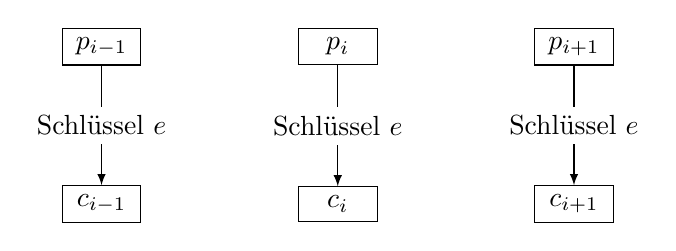
\begin{tikzpicture}
    \tikzstyle{opmode} = [draw, rectangle, minimum width = 1cm]
    \tikzstyle{la} = [-latex]
    \tikzstyle{label} = [fill=white]
    \node[opmode] (pi-1) at (-3, 1) {$p_{i-1}$};
    \node[opmode] (pi) at (0, 1) {$p_{i}$};
    \node[opmode] (pi+1) at (3, 1) {$p_{i+1}$};
    \node[opmode] (ci-1) at (-3, -1) {$c_{i-1}$};
    \node[opmode] (ci) at (0, -1) {$c_{i}$};
    \node[opmode] (ci+1) at (3, -1) {$c_{i+1}$};
    \draw[la] (pi-1) -- node[label] {Schlüssel $e$} (ci-1);
    \draw[la] (pi) -- node[label] {Schlüssel $e$} (ci);
    \draw[la] (pi+1) -- node[label] {Schlüssel $e$} (ci+1);
   \end{tikzpicture}
  \end{center}
  \caption{Der ECB-Mode.}
  \end{figure}
 \item \emphex{CBC-Mode} (cipher-block chaining): $c_i := E_e(p_i + c_{i-1})$ für alle $i \geq 1$
   \begin{figure}
\begin{center}
   \begin{tikzpicture}
    \tikzstyle{opmode} = [draw, rectangle, minimum width = 1cm]
    \tikzstyle{la} = [-latex]
    \tikzstyle{label} = [fill=white]
        \tikzset{cross/.style={cross out, draw, 
         minimum size=2*(#1-\pgflinewidth), 
         inner sep=0pt, outer sep=0pt, rotate = 45}}
    \node[opmode] (pi-1) at (-4, 1) {$p_{i-1}$};
    \node[opmode] (pi) at (0, 1) {$p_{i}$};
    \node[opmode] (pi+1) at (4, 1) {$p_{i+1}$};
    \node[opmode] (ci-1) at (-4, -2) {$c_{i-1}$};
    \node[opmode] (ci) at (0, -2) {$c_{i}$};
    \node[opmode] (ci+1) at (4, -2) {$c_{i+1}$};
    \node[cross=4pt] (oi-1) at (-4, 0) {};
    \node[cross=4pt] (oi) at (0, 0) {};
    \node[cross=4pt] (oi+1) at (4, 0) {};
    \draw (-4, 0) circle (5pt);
    \draw (0, 0) circle (5pt);
    \draw (4, 0) circle (5pt);
    \draw[la] (pi-1) -- (oi-1);
    \draw[la] (pi) -- (oi);
    \draw[la] (pi+1) -- (oi+1);
    \draw[la] (oi-1) -- node[label]  {Schlüssel $e$} (ci-1);
    \draw[la] (oi) -- node[label]  {Schlüssel $e$} (ci);
    \draw[la] (oi+1) -- node[label]  {Schlüssel $e$} (ci+1);
    \draw[la] (-7, -2) -- (-6, -2) -- (-6, 0) -- (oi-1);
    \draw[la] (ci-1) -- (-2, -2) -- (-2, 0) -- (oi);
    \draw[la] (ci) -- (2, -2) -- (2, 0) -- (oi+1);
    \draw[la] (ci+1) -- (6, -2);
   \end{tikzpicture}
  \end{center}
  \caption{Der CBC-Mode.}
   \end{figure}
 \item \emphex{CFB-Mode} (cipher feedback): $c_i := p_i + E_e(c_{i-1})$ für alle $i \geq 1$
 \begin{figure}
    \begin{center}
   \begin{tikzpicture}
    \tikzstyle{opmode} = [draw, rectangle, minimum width = 1cm]
    \tikzstyle{la} = [-latex]
    \tikzstyle{label} = [fill=white]
        \tikzstyle{label} = [fill=white]
        \tikzset{cross/.style={cross out, draw, 
         minimum size=2*(#1-\pgflinewidth), 
         inner sep=0pt, outer sep=0pt, rotate = 45}}
    \node[opmode] (pi-1) at (-4, 1) {$p_{i-1}$};
    \node[opmode] (pi) at (0, 1) {$p_{i}$};
    \node[opmode] (pi+1) at (4, 1) {$p_{i+1}$};
    \node[opmode] (ci-1) at (-4, -2) {$c_{i-1}$};
    \node[opmode] (ci) at (0, -2) {$c_{i}$};
    \node[opmode] (ci+1) at (4, -2) {$c_{i+1}$};
    \node[cross=4pt] (oi-1) at (-4, 0) {};
    \node[cross=4pt] (oi) at (0, 0) {};
    \node[cross=4pt] (oi+1) at (4, 0) {};
    \draw (-4, 0) circle (5pt);
    \draw (0, 0) circle (5pt);
    \draw (4, 0) circle (5pt);
    \draw[la] (pi-1) -- (oi-1);
    \draw[la] (pi) -- (oi);
    \draw[la] (pi+1) -- (oi+1);
    \draw[la] (oi-1) -- (ci-1);
    \draw[la] (oi) --  (ci);
    \draw[la] (oi+1) -- (ci+1);
    \draw[la] (-7, -2) -- (-6, -2) -- node[label] {Schlüssel $e$} (-6, 0) -- (oi-1);
    \draw[la] (ci-1) -- (-2, -2) -- node[label] {Schlüssel $e$} (-2, 0) -- (oi);
    \draw[la] (ci) -- (2, -2) -- node[label] {Schlüssel $e$} (2, 0) -- (oi+1);
    \draw[la] (ci+1) -- (6, -2);
   \end{tikzpicture}
  \end{center}
  \caption{Der CFB-Mode.}
  \end{figure}
 \item \emphex{OFB-Mode} (output feedback): $c_i := p_i + s_i$ für alle $i \geq 1$ mit $s_{0} = c_{0}$ und $s_i = E_e(s_{i-1})$ für alle $i \geq 1$   
 \begin{figure}
     \begin{center}
   \begin{tikzpicture}
    \tikzstyle{opmode} = [draw, rectangle, minimum width = 1cm]
    \tikzstyle{la} = [-latex]
        \tikzstyle{label} = [fill=white]
        \tikzstyle{label} = [fill=white]
        \tikzset{cross/.style={cross out, draw, 
         minimum size=2*(#1-\pgflinewidth), 
         inner sep=0pt, outer sep=0pt, rotate = 45}}
    \node[opmode] (si-1) at (-4, 1) {$s_{i-1}$};
    \node[opmode] (si) at (0, 1) {$s_i$};
    \node[opmode] (si+1) at (4, 1) {$s_{i+1}$};
    \node[opmode] (pi-1) at (-6, 0) {$p_{i-1}$};
    \node[opmode] (pi) at (-2, 0) {$p_{i}$};
    \node[opmode] (pi+1) at (2, 0) {$p_{i}$};
    \node[opmode] (ci-1) at (-4, -1) {$c_{i-1}$};
    \node[opmode] (ci) at (0, -1) {$c_{i}$};
    \node[opmode] (ci+1) at (4, -1) {$c_{i+1}$};
    \node[cross=4pt] (oi-1) at (-4, 0) {};
    \node[cross=4pt] (oi) at (0, 0) {};
    \node[cross=4pt] (oi+1) at (4, 0) {};
    \draw (-4, 0) circle (5pt);
    \draw (0, 0) circle (5pt);
    \draw (4, 0) circle (5pt);
    \draw[la] (pi-1) -- (oi-1);
    \draw[la] (pi) -- (oi);
    \draw[la] (pi+1) -- (oi+1);
    \draw[la] (si-1) -- (oi-1);
    \draw[la] (si) -- (oi);
    \draw[la] (si+1) -- (oi+1);
    \draw[la] (oi-1) -- (ci-1);
    \draw[la] (oi) --  (ci);
    \draw[la] (oi+1) -- (ci+1);
    \draw[la] (-7, 1) -- node [label] {Schlüssel $e$} (si-1);
    \draw[la] (si-1) -- node [label] {Schlüssel $e$} (si);
    \draw[la] (si) -- node [label] {Schlüssel $e$} (si+1);
    \draw[la] (si+1) -- (5, 1);
     \end{tikzpicture}
  \end{center}
  \caption{Der OFB-Mode.}
  \end{figure}
\end{enumerate}

\begin{example}[Verschlüsselungs-Modi]
 Als Blockchiffre wählen wir das One-Time-Pad mit Blocklänge $3$. Der Schlüssel sei $e = ([10], [8], [4]) \in ℤ_{26}^3$. Wir wählen $c_{0} = ([1], [1], [1])$ und verschlüsseln den Klartext 
 \begin{small}
 \[p = ([12], [7], [23], \quad [2], [17], [4], \quad [1], [9], [13]) \in ℤ_{26}^9\]
 \end{small}
 \begin{enumerate}
  \item im ECB-Mode: 
  \begin{small}
  \begin{align*} E_e(p) = &([12 +10], [7+8], [23+4], \quad [2+10], [17+8], [4+4], \quad [1+10], [9+8], [13+4]) \\
   = & ([22], [15], [1], \quad [12], [25], [8], \quad [11], [17], [17]) \in ℤ_{26}^9
   \end{align*}
   \end{small}
  Wir erhalten wieder die Vigenère-Chiffre mit Schlüssellänge $3$, nun aber für Klartexte beliebiger Länge.
   \item im CFB-Mode:
   
   Da die Blocklänge $3$ ist, erhalten wir 
   \begin{small}
   \[p_1 = ([12], [7], [23]), \; p_2 = ([2], [17], [4]) \text{ und } p_3 = ([1], [9], [13]).\]
   \end{small}
   Nun gilt 
   \begin{small}
   \begin{align*}
   c_1 = \;& p_1 + E_e(c_{0}) = ([12], [7], [23]) + [([1], [1], [1]) + [10], [8], [4])] &&= ([23], [16], [2]), \\
   c_2 = \;& p_2 + E_e(c_1) = ([2], [17], [4]) + [([23], [16], [2]) + [10], [8], [4])] &&= ([9], [15], [10]), \\
   c_3 = \;& p_3 + E_e(c_2) = ([1], [9], [13]) + [([9],[15], [10]) + [10], [8], [4])] &&= ([20], [19], [27]).
   \end{align*}
   \end{small}
   Insgesamt erhalten wir den Chiffretext
   \begin{small}
    \[c = ([23], [16], [2], \quad [9], [15], [10], \quad [20], [19], [27]) \in ℤ_{26}^9.\]
   \end{small}

 \end{enumerate}
\end{example}


\begin{exercise}
 \begin{enumerate}
  \item Wir wählen den Schlüssel $e = ([1], [0], [1], [1]) \in ℤ_2^4$, außerdem $c_{0} = ([0], [0], [1], [1]) \in ℤ_2^4$ und den Klartext
  \[p = ([0], [1], [0], [0], \; [0], [1], [0], [0], \; [1], [1], [1], [0],\; [1], [0], [1], [1]) \in ℤ_2^{16}.\]
  Verschlüsseln Sie $p$ mit den Verschlüsselungsmodi ECB-, CBC-, CFB- und OFB-Mode unter Nutzung des Vernam-One-Time-Pads als zugrunde liegender Blockchiffre mit Blocklänge $4$. 
 
  Nehmen sie nun an, dass 
  \[c = ([1], [1], [0], [1], \; [1], [1], [0], [1], \; [0], [0], [1], [0],\; [1], [0], [0], [1]) \in ℤ_2^{16}\]
  mit $e$ und dem ECB-, CBC-, CFB- bzw. OFB-Mode verschlüsselt wurde, wieder mit dem Vernam-One-Time-Pad als Blockchiffre. Bestimmen Sie jeweils den Klartext.  
  \item Implementieren Sie die Verschlüsselungsmodi ECB-, CBC-, CFB- und OFB-Mode für beliebige Blockchiffren.
 \end{enumerate}

 
\end{exercise}



\section{AES}\label{sec:AES}

Der \emphex[AES]{Advanced Encryption Standard (AES)} ist ein flächendeckend genutztes Secret"=Key"=Kryptosystem. Der AES-Algorithmus ist frei verfügbar und darf ohne Lizenzgebühren eingesetzt werden. Er gilt bis heute als sicher. Die komplexeren Versionen von AES haben einen so guten Ruf, dass sie in den USA für staatliche Dokumente mit höchster Geheimhaltungsstufe zugelassen sind. Der erste theoretisch interessante Angriff wurde 2011 veröffentlicht. Dieser ist im Schnitt etwa um einen Faktor $4$ schneller als ein vollständiges Durchsuchen des Schlüsselraums. Diese Beschleunigung ist so gering, dass AES trotz des Wissens um diesen theoretischen Angriff weiterhin als sicher gilt.

% Für Primzahlen $p$ haben Sie in der Geometrie-Vorlesung bisher die endlichen Körper $(ℤ_p, +, \cdot)$ kennen gelernt. Diese haben $p$ Elemente. Tatsächlich gibt es für alle $p, n \in ℕ$ mit $p$ prim einen Körper mit $p^n$ Elementen. Im folgdenden Abschnitt werden wir solche Körper, die mit $\GF(256)$ bezeichnet werden, konstruieren.

Das Alphabet, auf dem AES arbeitet, ist ein endlicher Körper mit $256$ Elementen, der mit $\GF(2^8)$ bezeichnet wird. Dass $\GF(2^8)$ und nicht ein Ihnen bereits bekannter Körper $ℤ_p$ mit einer Primzahl $p \in ℕ$ für AES genutzt wird, liegt an der Arbeitsweise von Computern: 

Ein Verschlüsselungsalgorithmus soll schnell sein und wenig Speicher verbrauchen. Computer arbeiten auf Bits als kleinster Maßeinheit für Informationsgehalt. Ein Bit hat zwei Zustände, \emph{Ein} oder \emph{Aus}, die man in der Mathematik mit den Elementen von $ℤ_2$ ausdrückt. Die nächstgrößere Maßeinheit sind Bytes, die aus $8$ Bits bestehen. In der Mathematik ist ein Byte somit mit einem Element von $ℤ_2^8$ identifiziert, \zB stellt $(\ol 1, \ol 0, \ol 1, \ol 1, \ol 1, \ol 0, \ol 0, \ol 1) \in ℤ_2^8$ ein spezielles Byte dar. Stehen die Elemente von $ℤ_2^8$ für Bytes, nutzt man in der Regel die kürzere Notation $10111001$.

Um eine effiziente Implementierung zu gewährleisten, ist es daher naheliegend für AES ein Alphabet mit $256$ Buchstaben zu nutzen. Um auch komplexere Rechenoperationen, nämlich Divisionen auf dem Alphabet durchführen zu können, nutzt man die Struktur des Körpers $\GF(2^8) = \GF(256)$. 

Es gibt ein weiteres Argument für ein Alphabet mit $256$ Buchstaben (das allerdings auf dem ersten basiert): Unicode ist ein internationaler Standard, in dem langfristig für jedes Schriftzeichen (nicht nur das Standardalphabet, auch mathematische Symbole und arabische Zeichen) ein digitaler Code festgelegt wird. Die am weitesten verbreitete Codierung für Unicode-Zeichen ist UTF-$8$, eine Erweiterung von ASCII. Anfang $2015$ nutzen über $80\%$ der Webseiten UTF-$8$ zur Zeichencodierung. Die Buchstaben vieler westlicher Sprachen brauchen mit UTF-$8$ genau ein Byte Speicherplatz. Unter Nutzung von UTF-$8$ entsprechen damit häufig die Schriftzeichen im menschenlesbaren Text genau einem Buchstaben im Alphabet von AES. Beispielsweise wird das Wort \enquote{AES} nach der Codierung mit UTF-$8$ zu
\[01000001 \;\;\; 01000101 \;\;\; 01010011.\]
Dies wäre die Nachricht im Klartextraum, die im Anschluss mithilfe des AES-Algorithmus verschlüsselt wird. 

Obwohl AES auf dem endlichen Körper $\GF(2^8)$ als Alphabet arbeitet, verzichten wir in dieser in dieser Vorlesung auf die Konstruktion endlicher Körper. Interessierte Leser können die Ideen der Konstruktion in \ref{subsection:finitefields} nachlesen. Für unsere Zwecke ist der folgende Satz ausreichend, den wir ohne Beweis zitieren.

\begin{theorem}\label{thm:finiteFields}
 Seien $n \in ℕ$, $p \in \Primes$. Dann existiert ein Körper mit $p^n$ Elementen, der bis auf Isomorphie eindeutig ist. Wir bezeichnen diesen Körper mit $\GF(p^n)$.
\end{theorem}

Insbesondere existiert also ein Körper mit $2^8$ Elementen, nämlich $\GF(2^8)$, der als Alphabet für AES genutzt wird.

\begin{remark}
 Die Formulierung \enquote{bis auf Isomorphie eindeutig} bedeutet Folgendes: Sind $K_1$ und $K_2$ zwei Körper mit $p^n$ Elementen, dann sind $K_1$ und $K_2$ isomorph. Zwei isomorphe Körper $K_1$ und $K_2$ unterscheiden sich anschaulich nur in die Bezeichnung ihrer Elemente, die Rechenregeln für $+$ und $\cdot$ sind dieselben.
\end{remark}

\begin{remark}
Das $\GF$ in $\GF(p^n)$ steht für \enquote{Galois field}: Évariste Galois war im 19. Jahrhundert ein französischer Mathematiker, der auf dem Gebiet der Körpertheorie gearbeitet hat und die nach ihm benannte Galoistheorie begründet hat. Er hat u.\,a.~Körpererweiterungen untersucht, d.\,h.~das Zusammenspiel von Körpern, die wie $\R$ in $\Ce$ ineinander enthalten sind. \enquote{field} ist das englische Wort für Körper.
\end{remark}

\begin{notation}[Elemente des Körpers $\GF(2^8)$]\label{not:fieldVectorspace}
 Obwohl wir den Körper $\GF(2^8)$ nicht formal einführen, möchten wir Rechenoperationen darauf beschreiben, um AES vorstellen zu können. Wir benutzen folgende Bezeichnung für die Elemente von $\GF(2^8)$:
 \begin{enumerate}
\item Elemente von $ℤ_2^8$, z.\,B.~$([0],[1],[0],[1],[0],[0],[1],[0]) \in \GF(2^8)$
 \item zweistellige Hexadezimalzahlen, z.\,B. $\texttt{d2}$
 \end{enumerate}
 Wie üblich bezeichnen wir die Ziffern im Hexadezimalsystem, dem Stellenwertsystem zur Basis $16$, mit 
 \[\text{\texttt{0, 1, 2, 3, 4, 5, 6, 7, 8, 9, a, b, c, d, e, f}.}\]
 Die Zahlen \texttt{c} und \texttt{4c} im Hexadezimalsystem entsprechen beispielsweise den Zahlen $12$ und $4 \cdot 16 + 12 \cdot 1 = 76$ im Dezimalsystem.

 Die Umrechnung eines Elements in $ℤ_2^8$ in eine zweistellig Hexadezimalzahl funktioniert beispielhaft wie folgt:
 
 Der Vektor $(\ol 1, \ol 0, \ol 1, \ol 1, \ol 1, \ol 0, \ol 0, \ol 1) \in ℤ_2^8$ wird als die Binärzahl $10111001$ aufgefasst. Bei der Umwandlung ins Hexadezimalsystem gehen die ersten vier Stellen von $10111001$ auf die erste Stelle im Hexadezimalsystem, die letzten vier Stellen auf die zweite Stelle. $1011$ im Binärsystem ist $11$ im Dezimalsystem, also \texttt{b} im Hexadezimalsystem. $1001$ im Binärsystem ist $9$ im Dezimalsystem, also \texttt{9} im Hexadezimalsystem. Insgesamt erhalten wir \texttt{b9} als Hexadezimaldarstellung des Vektors $(\ol 1, \ol 0, \ol 1, \ol 1, \ol 1, \ol 0, \ol 0, \ol 1) \in ℤ_2^8$. 
 
 Die Addition auf $\GF(2^8)$ entspricht der Addition auf $ℤ_2^8$, die Multiplikation auf $\GF(2^8)$ führen wir nicht ein.
 \end{notation}

Von endlichen Körpern zurück zu AES: 

Der AES-Algorithmus ist ein Spezialfall der sogenannten \emph{Rijndael-Chiffre}, die von den Belgiern Joan Daemen und Vincent Rijmen in den $90$-ern entwickelt wurde. Es gibt mehrere Versionen des AES-Algorithmus, die sich durch die Schlüssellänge $\Nk = 16, 24, 32$ und die Anzahl der Runden 
\[\Nr = \begin{cases}
         10 & \text{ für } \Nk = 16,\\
         12 & \text{ für } \Nk = 24,\\
         14 & \text{ für } \Nk = 32\\
        \end{cases}
\]
unterscheiden. Um die Darstellung nicht unnötig kompliziert werden zu lassen, beschränken wir uns in dieser Vorlesung auf die Schlüssellänge $\Nk = 16$ und damit die Rundenanzahl $\Nr = 10$.

Wir modellieren AES als Blockchiffre:

Das Alphabet von AES ist $A = \GF(2^8)$, die Blocklänge ist $n = 16$, damit gilt für den Klartext- und den Chiffretextraum 
\[\mc P = \mc C = \GF(2^8)^{16};\]
ein Beispiel für einen Klartext (in Hexadezimaldarstellung) ist
\[\texttt{32 43 f6 a8 88 5a 30 8d 31 31 98 a2 e0 37 07 34} \; \; \in \mc P.\]
Der Schlüsselraum der hier beschriebenen Version von AES ist ebenfalls $\mc K = \GF(2^8)^{16}$.
 
Für einen Schlüssel $e \in \mc K$, \zB
\[\texttt{3d c3 16 a3 28 ba a0 fd 3e 32 92 52 e0 b7 0b b4} \; \; \in \mc K = \GF(2^8)^{16},\]
beschreiben wir nun den Verschlüsselungsalgorithmus $E_e: \mc P → \mc C$:

Aus dem Verschlüsselungsschlüssel $e \in \GF(2^8)^{16}$ wird ein expandierter Schlüssel 
\[\expand(e) = (e_1, \dots, e_{10}) \;\;\; \in (\GF(2^8)^{16})^{10} = \mc P^{10} = \mc C^{10}\]
erzeugt, \zB
\begin{center}
\begin{align*}
\texttt{29 ee cb 34 44 85 93 3a 5b d6 5c 47 9f 11 3a 70} & \\  
\texttt{32 43 f6 a8 88 5a 30 8d 31 31 98 a2 e0 37 07 34} & \\
\texttt{49 8f 52 43 1f e1 cb e2 bf 94 3c d0 30 f5 55 a0} & \\
\texttt{6e c2 63 7f 27 3b ee 7f f0 2f 74 ac 92 21 22 c6} & \\
\texttt{3b b9 73 ae c9 f1 7c 78 66 60 86 6e 85 9d 04 70} & \\
\texttt{ec 1a 11 21 0e 6b 86 1a a6 70 d5 04 a8 fc ff 5d} & \\
\texttt{0f de 2f aa 20 ce 47 5f da 09 42 22 b6 cc 2f ba} & \\
\texttt{db 7a 6a 30 7f e5 e2 07 52 94 24 4d 7c 19 62 37} & \\
\texttt{a8 fe c0 b7 58 16 8e 2c 4a de 6e 7c 8e eb 24 4a} & \\
\texttt{f0 34 ab 36 84 89 06 4e 29 3a 6b 0f 82 09 72 be} & \; \in \mc K^{10} = (\GF(2^8)^{16})^{10}.
 \end{align*}
 \end{center}
 Auf den verwendeten Algorithmus gehen wir in dieser Vorlesung nicht ein, stattdessen gehen wir davon aus, dass der expandierte Schlüssel $(e_1, \dots, e_{10})$ bereits vorliegt.

Die Verschlüsselungsfunktion $E_e$ durchläuft $\Nr = 10$ Runden, in denen jeweils die Transformationen \texttt{SubBytes}, \texttt{MixColumns}, \texttt{ShiftRows} und eine Addition erfolgen. Zusätzlich erfolgt eine Vor- und eine Nachbearbeitung. Die genauen Schritte, die $E_e$ zugrunde liegen, sind in Algorithmus \ref{alg:aes} aufgeführt. Wir beschreiben nun die Transformationen \texttt{SubBytes}, \texttt{MixColumns} und \texttt{ShiftRows}. 

\begin{algorithm}
 \begin{algorithmic}
  \Require Klartext $p \in \mc P = \GF(2^8)^{16}$, Schlüssel $e \in \mc K = \GF(2^8)^{16}$
  \Ensure Chiffretext $c = E_e(p) \in \mc C = \GF(2^8)^{16}$
  \State $(e_1, \dots, e_{10}) \gets \expand(e)$
  \State $c \gets p + e$
  \For{$i = 1, \dots, 9$} 
  \State $c \gets$ \texttt{SubBytes}$(c)$
  \State $c \gets$ \texttt{ShiftRows}$(c)$
  \State $c \gets$ \texttt{MixColumns}$(c)$
  \State $c \gets c + e_i$
  \EndFor
  \State $c \gets $ \texttt{SubBytes}$(c)$
  \State $c \gets $ \texttt{ShiftRows}$(c)$
  \State $c \gets c + e_{10}$
  \State \Return $c$
 \end{algorithmic}
 \caption{Advanced Encryption Standard (AES)}
\end{algorithm}\label{alg:aes}


\subsubsection{Die Transformation \texttt{SubBytes}}

Die Transformation \texttt{SubBytes} arbeitet buchstabenweise durch Verwürfelung der Buchstaben des Alphabets $\GF(2^8)$. Wir definieren die Abbildung
\[\sigma: \GF(2^8) → \GF(2^8), \;\; b ↦ A \cdot \textcolor{red}{b^{-1}} + c\]
durch

\[A = \begin{pmatrix}
   \ol 1 & \ol 0 & \ol 0 & \ol 0 & \ol 1 & \ol 1 & \ol 1& \ol 1 \\
   \ol 1 & \ol 1 & \ol 0 & \ol 0 & \ol 0 & \ol 1 & \ol 1& \ol 1 \\
   \ol 1 & \ol 1 & \ol 1 & \ol 0 & \ol 0 & \ol 0 & \ol 1& \ol 1 \\
   \ol 1 & \ol 1 & \ol 1 & \ol 1 & \ol 0 & \ol 0 & \ol 0& \ol 1 \\
   \ol 1 & \ol 1 & \ol 1 & \ol 1 & \ol 1 & \ol 0 & \ol 0& \ol 0 \\
   \ol 0 & \ol 1 & \ol 1 & \ol 1 & \ol 1 & \ol 1 & \ol 0& \ol 0 \\
   \ol 0 & \ol 0 & \ol 1 & \ol 1 & \ol 1 & \ol 1 & \ol 1& \ol 0 \\
   \ol 0 & \ol 0 & \ol 0 & \ol 1 & \ol 1 & \ol 1 & \ol 1& \ol 1 \\
  \end{pmatrix} \in ℤ_2^{8\times8} \text{ und } c = \begin{pmatrix}
							\ol 1 \\
							\ol 1 \\
							\ol 0 \\
							\ol 0 \\
							\ol 0 \\
							\ol 1 \\
							\ol 1 \\
							\ol 0
						      \end{pmatrix}.\]


Man kann zeigen, dass $\det A = \ol 1 \in ℤ_2$ gilt und dass $A$ somit invertierbar ist. Die Abbildung $\sigma$ ist nicht affin linear (man beachte das $b^{-1}$), was AES vor dem in Abschnitt \ref{sec:affineblockcipher} beschriebenen Known"=Plaintext"=Angriff auf affin lineare Blockchiffren schützt. 

Die Permutation $\sigma: \GF(2^8) → \GF(2^8)$, über die \texttt{SubBytes} definiert ist, kann wie in Abbildung \ref{fig:subbytes} tabelliert werden. Beispielsweise kann dort $\sigma(\texttt{1d}) = \texttt{a4}$ abgelesen werden.

\begin{figure}
\begin{center}
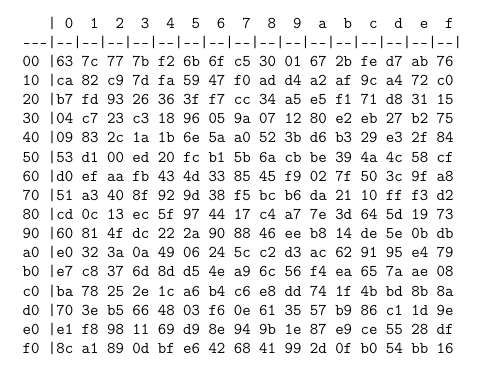
\includegraphics[scale=0.95]{subbytes}
\end{center}
 \caption{Tabellierung von \texttt{SubBytes}.}\label{fig:subbytes}
\end{figure}

Die Transformation \texttt{SubBytes} wendet die Abbildung $\sigma$ buchstabenweise an:
\[\texttt{SubBytes}(p_1, \dots, p_{16}) = (\sigma(p_1), \dotsc, \sigma(p_{16}))\]
für alle $(p_1, \dots, p_{16}) \in \GF(2^8)^{16} = \mc P = \mc C$.

Beispielsweise gilt
\begin{align*}
\texttt{SubBytes(}&\texttt{32 43 f6 a8 88 5a 30 8d 31 31 98 a2 e0 37 07 34)} \\
 =\;\;& \texttt{23 1a 42 c2 c4 be 04 5d c7 c7 46 3a e1 9a c5 18}.
\end{align*}

\subsubsection{Die Transformation \texttt{ShiftRows}}

Die Transformation \texttt{ShiftRows} permutiert die Buchstaben eines Blocks $p = (p_1, \dots, p_{16}) \in \GF(2^8)^{16}$:
\[\texttt{SubBytes}(p) = (p_1, p_6, p_{11}, p_{16}, p_5, p_{10}, p_{15}, p_4, p_9, p_{14}, p_3, p_8, p_{13}, p_2, p_7, p_{12})\]
Beispielsweise gilt:
\begin{align*}
\texttt{ShiftRows(}&\texttt{23 1a 42 c2 c4 be 04 5d c7 c7 46 3a e1 9a c5 18)}\\
 =\;\;& \texttt{23 be 46 18 c4 c7 c5 c2 c7 9a 42 5d e1 1a 04 3a}\\
 \hline
 	           &\texttt{01 02 03 04 05 06 07 08 09 10 11 12 13 14 15 16} 
\end{align*}

\subsubsection{Die Transformation \texttt{MixColumns}}

Die Transformation \texttt{MixColumns} operiert auf Blöcken der Länge $4$, also auf $\GF(2^8)^4$. Wir definieren die lineare Abbildung
\[S: \GF(2^8)^4 → \GF(2^8)^4, \;\; \begin{pmatrix}
                                              p_1 \\
                                              p_2 \\
                                              p_3 \\
                                              p_4 
                                             \end{pmatrix}
 ↦ \begin{pmatrix}
              \texttt{02} & \texttt{03} & \texttt{01} & \texttt{01} \\
              \texttt{01} & \texttt{02} & \texttt{03} & \texttt{01} \\
              \texttt{01} & \texttt{01} & \texttt{02} & \texttt{03} \\
              \texttt{03} & \texttt{01} & \texttt{01} & \texttt{02}
             \end{pmatrix} 
             \begin{pmatrix}
              p_1 \\
              p_2 \\
              p_3 \\
              p_4
             \end{pmatrix}.
\]
Die Einträge der Matrix sind Hexadezimalzahlen, die für die entsprechenden Elemente von $\GF(2^8)$ stehen.

Die Transformation \texttt{MixColumns} wendet die $\GF(2^8)$-lineare Abbildung $S$ blockweise an:
\[\texttt{MixColumns}(p) = \(S(p_1, p_2, p_3, p_4), S(p_5, p_6, p_7, p_8), S(p_9, p_{10}, p_{11}, p_{12}), S(p_{13}, p_{14}, p_{15}, p_{16})\)\]
für alle $(p_1, \dots, p_{16}) \in \GF(2^8)^{16} = \mc P = \mc C$.

Da die Multiplikation auf $\GF(2^8)$ nicht eingeführt wurde, kann kein Beispiel für die Abbildung $S$ und die Transformation $\texttt{MixColumns}$ angegeben werden.

\subsubsection{Dekodierung}

Um einen mit AES verschlüsselten Text zu dechiffrieren, muss man den AES-Algorithmus invertieren. Dazu geht man den Algorithmus von hinten nach vorne durch und kehrt die durchgeführten Schritte um. Dies ist möglich, da alle genutzten Transformationen \texttt{SubBytes}, \texttt{MixColumns}, \texttt{ShiftRows} und auch die Addition invertierbar sind:

\begin{itemize}
 \item \texttt{SubBytes} arbeitet buchstabenweise durch (bijektive) Verwürfelung des Alphabets. Diese Verwürfelung kann umgekehrt werden.
 \item \texttt{ShiftRows} permutiert die Buchstaben eines Textes, ist also bijektiv. Die Permutation der Buchstaben kann umgekehrt werden.
 \item \texttt{MixColumns} arbeitet blockweise als invertierbare lineare Abbildung $S: \GF(2^8)^4 → \GF(2^8)^4$. Es existiert also eine (blockweise arbeitende) inverse lineare Abbildung.
\end{itemize}

\subsubsection{Kryptoanalyse}

Eine Kryptoanalyse von AES ist schwierig und aufwendig. Das liegt nicht daran, dass die einzelnen Schritte komplex und undurchsichtig sind, sondern daran, dass sehr viele Schritte während des Algorithmus durchlaufen werden. Erst durch das Aneinanderreihen der einzelnen Transformation in mehreren Runden wird AES komplex und undurchsichtig.

Die einzelnen durchgeführten Schritte haben sogar eine sehr einfach Struktur: Bis auf \texttt{SubBytes} sind alle Transformationen affin linear und wären für sich allein genommen zu Knacken. Daher ist der Einsatz von \texttt{SubBytes} so wichtig, um AES vor dem in Kapitel \ref{sec:affineblockcipher} beschriebenen Known-Plaintext-Angriff zu schützen.

Gerade diese Einfachheit der einzelnen Transformationen ist wiederum eine Stärke von AES: Sie garantiert, dass AES effizient arbeitet, d.\,h.~wenig Speicher und wenig Rechenzeit benötigt. Neben der Sicherheit des Algorithmus war das ein Hauptkriterium bei der Auswahl von AES im 1997 vom NIST ausgeschriebenen Wettbewerb.

\section{Exkurs: Endliche Körper}\label{subsection:finitefields}

Für interessierte Leser beschreiben wir aufbauend auf \cite{gathmann2010} die Konstruktion endlicher Körper. Dazu führen wir zuerst den Polynomring und Teilbarkeitsbegriffe ein. Im Folgenden sei ein Ring stets kommutativ und mit Eins.

\subsubsection{Der Polynomring}

\begin{definition}[Polynome]\label{def:polynom}
 Sei $R$ ein Ring. 
 \begin{enumerate}
  \item Ein \emphex[Polynom]{Polynom in einer Variablen über $R$} ist ein Ausdruck der Form
 \[a_nt^n + a_{n-1}t^{n-1} + \dotsc + a_1t +a_0\]
 mit \emph{Koeffizienten} $a_n$, \dots, $a_0 \in R$ und $n \in \N$. Wir fassen dabei $t$ als \emphex{formale Variable} auf. Natürlich könnte man hier auch einen anderen Buchstaben als formale Variable wählen, in diesem Exkurs werden wir die formale Variable eines Polynoms jedoch immer mit $t$ bezeichnen.
 
 Wir definieren $R[t]$ als die Menge aller Polynome über $R$. 
 
 \item Sind $f = \sum_{k=0}^{n_f} a_kt^k$ und $g = \sum_{k_0}^{n_g} b_kt^k$ Polynome, so definieren wir ihre Summe $f+g$ und ihr Produkt $f \cdot g$ als die Polynome
 \begin{equation}
 \begin{aligned}
  && f + g & := \sum_{k = 0}^{n_f} (a_k + b_k) t^k \\
  &\text{und} & f \cdot g& := \sum_{m = 0}^{n_f + n_g} \(\sum_{k + l = m} \(a_k + b_l\) \) t^m. 
 \end{aligned}
 \end{equation}
 \end{enumerate}
\end{definition}


\begin{remark}
  Man beachte, dass die Multiplikation von Polynomen genauso eingeführt wurde, wie man es erwarten würde, wenn man diese formalen Summen naiv ausmultiplizieren würde: dann wäre nämlich
  \begin{align}
   \(\sum_{k=0}^{n_f} a_kt^k\) \cdot \(\sum_{l = 0}^{n_g} b_lt^l\) & = (a_0 + a_1t + a_2t^2 + \dotsc) \cdot (b_0 + b_1t + b_2t^2 + \dotsc) \\
   & = a_0b_0 + (a_0b_1 + a_1b_0)t + (a_0b_2 + a_1b_1 + a_2b_0)t^2 + \dotsc \\
   & = \sum_{m = 0}^{n_f + n_g} \(\sum_{k + l = m} (a_k + b_l) \) t^m,
  \end{align}
 was genau die obige Definition ist. 
  \end{remark}
  
\begin{example}
 Über einem Ring $R$ betrachten wir das Polynom
 \[f = 1 + 1t + 1t^2 + \dotsc + 1t^n \in R[t].\]
 Dann ist nach \ref{def:polynom} die Summe von $f$ mit sich selbst
 \[f + f = 2f = \sum_{k=0}^n (1 + 1)t^n = \sum_{k=0}^n 2t^n\]
 und das Produkt von $f$ mit sich selbst
 \[f \cdot f = f^2 = \sum_{m=0}^{2n} \(\sum_{k + l = m} 1 \cdot 1\) t^n = \sum_{m = 0}^{2n} (m+1)t^n,\]
 da die Summe über $k$ und $l$ aus $m + 1$ Summanden besteht.
\end{example}

\begin{notation}
 Aus naheliegenden Gründen lässt man Monome von der Form $0t^n$ bei der Notation von Polynomen häufig weg und schreibt $t^n$ für $1t^n$.
\end{notation}

\begin{theorem}
 Für jeden Körper $R$ ist die Menge $R[t]$ aller Polynome zusammen mit den Verknüpfungen aus Definition \ref{def:polynom} ein Ring. $R$ ist ein Unterring von $R[t]$, insbesondere sind $0 \in R$ und $1 \in R$ die neutralen Elemente in $R[t]$ bezüglich Addition und Multiplikation.
\end{theorem}

\begin{definition}[Grad, Leitkoeffizient]
 Wieder sei $R$ ein Ring. 
 \begin{enumerate}
  \item Ist $f \in R[t]$ ein Polynom mit $f ≠ 0$, so können wir $f$ eindeutig als 
  \[f = a_0 + a_1t + \dotsc + a_nt^n\]
  mit $n \in \N$ und $a_n ≠ 0$ schreiben. Die Zahl $n$, also der höchste in $f$ auftretende Exponent von $t$ wird der \emphex[Grad]{Grad von $f$} genannt und als $\deg f$ geschrieben (die Bezeichnung kommt vom englischen Wort \enquote{degree}). Dann heißt $a_n \in R$ Leitkoeffizient von $f$.
%   Man nennt $f$ \emphex[Polynom!normiert]{normiert}, wenn dieser Leitkoeffizient gleich $1$ ist.
  \item Ein Polynom $a_0 \in R \subset R[t]$ vom Grad $0$ heißt \emphex[Polynom!konstant]{konstantes Polynom}.
 \end{enumerate}
\end{definition}


\begin{definition}[Polynomfunktion]
 Ist $f = a_0 + a_1t + \dotsc + a_nt^n$ ein Polynom über dem Körper $K$ und ist $x \in R$, so heißt das Ringelement 
 \[f(x):= a_0 + a_1x + \dotsc + a_nx^n \; \; \; \in R\]
 der \emphex[Polynom!Wert]{Wert von $f$ in $x$}. die zugehörige Funktion $R → R$, $x ↦ f(x)$, wird eine \emphex{Polynomfunktion} genannt. Ist $f(x) = 0 \in R$, so heißt $x \in R$ eine \emphex[Nullstelle]{Nullstelle von $f$}.
\end{definition}

\begin{example}
 Jedes Polynom $f$ über $R$ bestimmt eine Polynomfunktion. Zwei verschiedene Polynome können dabei dieselbe Polynomfunktion bestimmen: Das Polynom $t^2 + t \in \Z_2[x]$ hat in jedem Element von $\Z_2$ den Wert Null. Während die beiden \emph{Polynome} $t^2 + t \in \Z_2[t]$ und $\ol 0 \in \Z_2[t]$ verschieden sind, sind die beiden zugehörigen Polynomfunktionen $t ↦ t^2 + t$ und $t ↦ \ol 0$ gleich. Man beachte, dass man deshalb einer \emph{Polynomfunktion} in der Regel keinen eindeutigen Grad zuweisen kann. Polynome verhalten sich hier also besser als Polynomfunktionen.
 
 Man kann allerdings zeigen, dass Polynome und Polynomfunktionen über Körpern mit unendlich vielen Elementen (also \zB $ℚ$, $ℝ$, $ℂ$) übereinstimmen. In diesem Fall macht es also keinen Unterschied, ob wir bei Polynomen an Funktionen oder an die formalen Ausdrücke aus \cref{def:polynom} denken. 
\end{example}

\subsubsection{Teilbarkeit im Ringen}

\begin{definition}[Teilbarkeit]
Sei $R$ ein kommutativer Ring mit $1$ und seien $a, b \in R$. 
\begin{itemize}
 \item Man sagt \emph{$a$ teilt $b$} und schreibt $a \mid b$, wenn ein $c \in R$ existiert, das $a \cdot c = b$ erfüllt. 
 \item Das Element $a$ heißt \emphex{Einheit}, wenn ein $c \in R$ existiert mit $a \cdot c = 1 \in R$. Die Menge aller Einheiten von $R$ wird mit $R^*$ bezeichnet und heißt \emphex[Einheitengruppe]{Einheitengruppe von $R$}.
 \item Das Element $a$ heißt \emphex{Nullteiler}, wenn ein $c \in R$ existiert mit $a \cdot c = 0 \in R$.
 \item Der Ring $R$ heißt \emphex{Integritätsring}, wenn er außer der Null keine Nullteiler besitzt, d.\,h. wenn für alle $x, y \in R$ gilt: Ist $ab = 0$, so ist bereits $a = 0$ oder $b = 0$.
\end{itemize}
\end{definition}

\begin{example}\label{expl:kintdomain}
 Ein Körper $K$ ist ein Integritätsring: Angenommen es würden Elemente $0 ≠ a, b \in K$ existieren, die $a \cdot b = 0$ erfüllen. Dann hätte $a$ ein Inverses $a^{-1}$ bezüglich der Multiplikation, und wir erhalten den Widerspruch $a^{-1} \cdot a \cdot b = b = 0$.
\end{example}


\begin{exercise}\label{ex:degree}
 Sei $R$ ein Integritätsring. Zeigen Sie:
 \begin{enumerate}
  \item Sind $0 ≠ f, g \in R[t]$ Polynome über $R$, so gilt
 \[\deg(f + g) \leq \max\{\deg f, \deg g\} \text{ und } \deg (f \cdot g) = \deg f + \deg g.\]
 \item  Es existiert ein Ring $R$ und Polynome $0 ≠ f, g \in R[t]$ mit $\deg (f \cdot g) < \deg f + \deg g$. Ein Tipp: Der Ring $R$ kann in diesem Fall kein Integritätsring, also insbesondere kein Körper sein.
 \end{enumerate}
\end{exercise}

\begin{exercise}[Einheitengruppe des Polynomrings]\label{ex:groupofunits}
 Sei $R$ ein Integritätsring. Zeigen Sie, dass die Einheitengruppe des Polynomrings über $R$ durch $R[t]^* = R^*$ gegeben ist. 
\end{exercise}

\begin{definition}[Primelemente und irreduzible Elemente]
 Sei $R$ ein Integritätsring und $p \in R$ mit $p ≠ 0$ und $p ≠ R^*$. 
 \begin{enumerate}
  \item $p$ heißt \emphex{irreduzibel}, wenn für alle $a, b \in R$ mit $p = a \cdot b$ gilt, dass $a \in R^*$ oder $b \in R^*$ eine Einheit ist. Andernfalls heißt $p$ \emphex{reduzibel}.
  \item $p$ heißt \emphex{prim}, wenn für alle $a, b \in R$ mit $p \mid a \cdot b$ gilt, dass $p \mid a$ oder $p\mid b$.
 \end{enumerate}

\end{definition}

\begin{lemma}
In einem Integritätsring ist jedes Primelement irreduzibel.
\end{lemma}

\begin{remark}
 Die Umkehrung dieses Lemmas gilt nicht: Es gibt Integritätsringe, in denen nicht alle irreduziblen Elemente prim sind.
\end{remark}

\subsubsection{Teilbarkeit im Polynomring}

Bezüglich der Teilbarkeit ist in Polynomringen vieles einfacher als in allgemeinen Ringen. Das liegt im Wesentlichen daran, dass man Polynome mit Rest durcheinander teilen kann. Das Verfahren der Division mit Rest sollte aus der Geometrie-Vorlesung bekannt sein.

\begin{theorem}[Polynomdivision]\label{thm:polynomdivision}
 Sind $f, g \in K[t]$ Polynome mit $g ≠ 0$, so gibt es stets Polynome $q, r \in K[t]$ mit $f = qg + r$ und $\deg r < \deg g$.
\end{theorem}

\begin{theorem}\label{thm:ufd}
 Sei $K$ ein Körper und $0 ≠ f \in K[t]$ ein Polynom mit $f \notin K[t]^*$. Dann hat $f$ eine \emphex[Primfaktorzerlegung!eindeutig]{eindeutige Primfaktorzerlegung}, d.\,h.:
 
 \begin{enumerate}
  \item Es gibt ein $n \in \N$ und Primelemente $p_1, \dots, p_n \in R$, so dass $a = p_1 \cdot \dotsc \cdot p_n$ gilt. Eine solche Darstellung heißt \emphex[Primfaktorzerlegung]{Primfaktorzerlegung von $f$}.
  \item Die Darstellung aus 1. ist \enquote{bis auf Reihenfolge und bis auf Multiplikation mit Einheiten eindeutig}.
 \end{enumerate}
\end{theorem}

\begin{lemma}
 Sei $K$ ein Körper und $f \in K[t]$. Dann ist $f$ genau dann prim, wenn es irreduzibel ist.
\end{lemma}

\begin{exercise}\label{ex:const->prime}
 Sei $K$ ein Körper und $p = t - a \in K[t]$ ein konstantes Polynome. Man zeige, dass $f$ dann irreduzibel ist.
\end{exercise}

\begin{corollary}[Abspalten von Nullstellen in Polynomen] \label{cor:polyRoots}
 Es sei $K$ ein Körper und $0 ≠ f \in K[t]$ ein Polynom vom Grad $n \in \N_{\geq 0}$.
 \begin{enumerate}
 \item Ist $a \in K$ eine Nullstelle von $f$, so gilt $x-a \mid f$.
 \item Das Polynom $f$ hat höchstens $n$ Nullstellen.
 \end{enumerate}
\end{corollary}
% \begin{proof}
%  \begin{enumerate}
%   \item Gemäß Satz \ref{thm:polynomdivision} existieren Polynome $q, r \in K[t]$ mit $f = (t-a)q + r$ mit $\deg r < \deg (t-a) = 1$. Inbesondere ist $r$ somit ein konstantes Polynom. Setzen wir in diese Gleichung den Wert $a$ ein, so erhalten wir (da $a$ Nullstelle von $f$ ist)
%  \[0 = f(a) = q(a)(a-a) + r(a) = r(a) \;\;\;\in K.\]
%  Da $r$ ein konstantes Polynom ist, dessen Wert an einer Stelle $a$ gleich Null ist, muss $r$ bereits das Nullpolynom sein. Also ist $f = q(t-a)$, d.\,h. $t-a \mid f$.
% \item Wir zeigen die Aussage mit Induktion über $n = \deg f$.
% \begin{itemize}
%  \item $n=0$: in diesem Fall ist die Aussage trivial, da ein konstantes Polynom $f ≠ 0$ natürlich keine Nullstellen besitzt.
%  \item $n -1 → n$: Als Induktionsvoraussetzung nehmen wir an, dass jedes Polynom über $K$ vom Grad $n-1 \in \N$ maximal $n-1$ Nullstellen hat. Hat $f$ mit $\deg f = n$ keine Nullstellen, so sind wir fertig. Ist andernfalls $a \in K$ eine Nullstelle von $f$, so können wir dieses Polynom nach 1. als $(t-a) \cdot g$ für ein $g \in K[t]$ schreiben. Gemäß der Gradformel aus Aufgabe \ref{ex:degree} hat $g$ Grad $n-1$ und damit nach Induktionsvoraussetzung maximal $n-1$ Nullstellen.
%  
%  Für jede Nullstelle $a'$ von $f$ gilt nach 1., dass $x-a'$ ein Teiler von $f$ ist, und nach Aufgabe \ref{ex:const->prime} und Beispiel \ref{expl:kintdomain}, dass $t-a'$ prim ist. Folglich ist $t - a'$ entweder ein Teiler von $t-a$ oder aber ein Teiler von $g$. Im ersten Fall ist $a' = a$. Im zweiten Fall ist $a'$ eine der maximal $n-1$ Nullstellen von $g$. 
%  \end{itemize}
%  \end{enumerate}
% \end{proof}


\begin{example}
 \begin{enumerate}
  \item Wir zeigen, dass $f = t^2 + t + 1 \in \Z_2[t]$ irreduzibel ist: Wäre $f$ reduzibel, so müsste $f$ nach Aufgabe \ref{ex:degree} Produkt von zwei Polynomen vom Grad $1$ sein. Dann hätte $f$ eine Nullstelle in $\Z_2$. Es gilt aber $f(\ol 0) = f(\ol 1) = \ol 1 \in \Z_2$. 
  \item Das Polynom $f = t^2 + \ol 1$ ist reduzibel in $\Z_2[t]$: Es gilt $(t + \ol 1)(t+ \ol 1) = t^2 + \ol 2t + \ol 1 \in \Z_2[t]$, wobei $t + \ol 1 \in \Z_2[t]$ gemäß \ref{ex:groupofunits} keine Einheit ist.
 \end{enumerate}
\end{example}

\begin{remark}[Größter gemeinsamer Teiler]\label{rem:ggT}
 Analog zu $\Z$ sind im Polynomring $K[t]$ über einem Körper $K$ \emphex[Teiler!größter gemeinsamer]{größte gemeinsame Teiler $\ggT(f, g)$ zweier Polynome $f, g$} definiert: 
 
 Ein Polynom $d \in K[t]$ heißt größter gemeinsamer Teiler von $f$ und $g$, wenn $d$ gemeinsamer Teiler von $f$ und $g$ ist und wenn für alle gemeinsamen Teiler $h$ von $f$ und $g$ auch $h \mid d$ gilt. Man kann zeigen, dass zwei Polynome  $f, g$ immer größte gemeinsame Teiler besitzen. In der Regel sind diese allerdings nicht eindeutig. Wie im Fall von $\Z$ kann ein größter gemeinsamer Teiler $d$ von $f$ und $g$ mithilfe des aus der Geometrie-Vorlesung bekannten erweiterten euklidischen Algorithmus bestimmt und als Linearkombination 
 \[d = a_1f + a_2g\]
 von $f$ und $g$ über $K[t]$ dargestellt werden, d.\,h. $a_1, a_2 \in K[t]$. 
\end{remark}

\begin{exercise}
 Bestimmen Sie mithilfe des erweiterten euklidischen Algorithmus einen größten gemeinsamen Teiler von $t^3 + \ol 1 \in \Z_2[t]$ und $t^3 + t^2 + t \in \Z_2[t]$. Stellen sie diesen Teiler als Linearkombination von $f$ und $g$ über $K[t]$ dar.
\end{exercise}

\subsubsection{Konstruktion endlicher Körper}

Die Elemente des endlichen Körpers, der nun konstruiert wird, sind Restklassen in $\Z_p[t]$ modulo eines Polynoms $f$ über $\Z_p$. Die Konstruktion dieser Restklassen entspricht der Konstruktion von Restklassen in $\Z$ modulo $n \in \N$.

\begin{definition}[Restklassenring modulo $(f)$]
Sei $K$ ein Körper und $f, g \in K[t]$. Wir bezeichnen mit $(f) := f \cdot K[t] := \{f \cdot h\mid h \in K[t]\}$ die Menge aller Vielfachen von $f$ und nennen $(f)$ das \emphex[Erzeugnis]{Erzeugnis von $f$}. Die \emphex[Restklasse]{Restklasse in $K[t]$ von $g$ modulo $f$} ist definiert als 
\[g + (f) = g + f \cdot K[t] := \{g + f \cdot h\mid h \in K[t]\}.\]
Sei $h \in g + (f)$ ein Polynom. Dann nennen wir $h$ einen \emphex[Repräsentant]{Repräsentanten von $g + (f)$}.

Die Menge aller Restklassen in $K[t]$ modulo $f$ bezeichnen wir mit $K[t]/(f)$ und nennen sie den \emphex[Restklassenring]{Restklassenring von $K[t]$ modulo $f$}. 
\end{definition}

\begin{theorem}\label{thm:quotientring}
 Sei $K$ ein Körper und $f \in K[t]$. Dann bildet die Menge der Restklassen $K[t]/(f)$ mit folgenden Operationen einen Ring $(K[t], +, \cdot)$:
 \begin{align}
 (g_1 + (f)) + (g_2 + (f)) & := g_1 + g_2 + (f) \\
 (g_1 + (f)) \cdot (g_2 + (f)) & := g_1 \cdot g_2 + (f)
 \end{align}
 
 Ist $f$ irreduzibel, dann ist $K[t]/(f)$ sogar ein Körper.
\end{theorem}

\begin{remark}
 Insbesondere ist $0 + (f) = (f)$ das neutrale Element der Addition in $K[t]/(f)$ und $1 + (f)$ das neutrale Element der Multiplikation. Damit ist $-g_1 + (f)$ das zu $g_1 + (f)$ inverse Element bezüglich $+$.
\end{remark}

\begin{remark}
 Man beachte, dass \enquote{$+$} in \cref{thm:quotientring} für drei verschiedenen Operationen steht: für die Addition auf $K[t]$, für die Addition auf $K[t]/(f)$ und für die Summe von einem Polynom $g \in K[t]$ und der Menge von Polynomen $(f)$. Da alle diese Operationen auf die Addition in $K[t]$ zurück geführt werden, ist diese Vereinheitlichung der Schreibweise sinnvoll und praktisch. Analog steht $\cdot$ für zwei verschiedene Operationen: für die Multiplikation auf $K[t]$ und die auf $K[t]/(f)$.
\end{remark}

\begin{example}
 Wir betrachten den Körper $K = \Z_2$ und das Polynom $f = t$. 
 
 Die Restklasse $\ol 0 + (t) = \{\ol 0 + t \cdot h\mid h \in \Z_2[t]\}$ enthält alle Polynome, die ein Vielfaches von $t$ sind, \zB gilt 
 \[t^5 + t^3 = \ol 0 + t \cdot (t^4 + t^2) \in \ol 0 + (t).\]
 Dahingegen enthält $\ol 1 + (t) = \{\ol 1 + t \cdot h\mid h \in K[t]\}$ alle Polynome, die sich um $\ol 1$ von einem Vielfachen von $t$ unterscheiden. 
 
 Insgesamt gilt $\Z_2[t]/(t) = \{f + (t)\mid f \in K[t]\} = \{\ol 0 + (t), \ol 1 + (t)\}$: 
 
 Jedes $g = a_0 + a_1t + \dotsc + a_nt^n \in Z_2[t]$ ist wegen $a_0 \in \{\ol 0, \ol 1\} = \Z_2$ entweder ein Vielfaches von $t$ oder unterscheidet sich um $\ol 1$ von einem Vielfachen von $t$.
 
 Da $t$ irreduzibel ist, ist $\Z_2[t]/(t)$ außerdem ein Körper. Er ist isomorph zu $\Z_2$.
\end{example}

Wir gehen nun der Frage nach, was die Menge der Restklassen modulo $f$ anschaulich darstellt. Dazu stellen wir einige Rechenregeln für die oben definierten Restklassen auf:

\begin{lemma}\label{lem:propquotring}
 Seien $K$ ein Körper und $f, g_1, g_2 \in K[t]$. Dann gilt:
 \begin{enumerate}
  \item $(a) = K[t]$ für alle konstanten Polynome $a \in K^*$
  \item $g_1 + K[t] = K[t]$
  \item $g_1 + (f) = 0 + (f) \;\;\; \Leftrightarrow \;\;\; g_1 \in (f)$
  \item $g_1 + (f) = g_2 + (f) \;\;\; \Leftrightarrow \;\;\; g_1 - g_2 \in (f)$
 \end{enumerate}
\end{lemma}
\begin{proof}
 \begin{enumerate}
  \item Die Abbildung $K[t] → K[t]$, $h ↦ a \cdot h$ ist bijektiv mit Bild $K[t] = \{a \cdot h\mid h \in K[t]\} = (a)$.
  \item Die Abbildung $K[t] → K[t]$, $h ↦ g + h$ ist bijektiv mit Bild $K[t] = g + K[t]$.
  \item \enquote{$\Rightarrow$}: Es gelte $g_1 + (f) = 0 + (f)$, also $\{g_1 + f⋅ h\mid h \in K[t]\} = \{f \cdot h\mid h \in K[t]\}$. Insbesondere gilt dann 
  \[g_1 = g_1 + f \cdot 0 \in \{f \cdot h\mid h \in K[t]\} = (f).\]
  
  \enquote{$\Leftarrow$} Wegen $g_1 \in (f) = \{f \cdot h\mid h \in K[t]\} $ existiert ein $h_1 \in K[t]$ mit $g_1 = f \cdot h_1$. Wegen der 2. Eigenschaft gilt $\{h_1 + h \mid h \in K[t]\} = \{h\mid h \in K[t]\}$, und wir folgern
  \[g_1 + (f) = \{f \cdot h_1 + f⋅ h\mid h \in K[t]\} = \{f \cdot (h' + h)\mid h \in K[t]\} = \{f \cdot h\mid h \in K[t]\} = (f).\]
  \item \enquote{$\Rightarrow$}: Es gelte $g_1 + (f) = g_2 + (f)$. Daraus folgt
  \[0 + (f) = (-g_2 + (f)) + (g_1 + (f)) = -g_2 + g_1 + (f).\]
  Mit 3. erhalten wir $g_1-g_2 \in (f)$.
  
  \enquote{$\Leftarrow$}: Aus $g' := g_1 - g_2 \in (f)$ folgern wir mit der 3. Eigenschaft
 \[g_1 + (f) = g_2 + g' + (f) = g_2 + (f).\]
  
 \end{enumerate}
\end{proof}


Nun sind wir in der Lage zwei sich ergänzende Anschauungen des Restklassenrings zu gewinnen.

Zuerst einmal stellen wir mit Satz \ref{thm:quotientring} fest, dass wir im Restklassenring im Prinzip wie im Polynomring rechnen können: zwei Restklassen $g_1 + (f)$ und $g_2 + (f)$ werden addiert, indem man ihre Repräsentanten zu $g_1+g_2$ addiert und dann die zugehörige Restklasse $g_1 + g_2 + (f)$ berechnet; genauso für die Multiplikation.

Zum anderen gibt es Unterschiede zum Polynomring:

\begin{enumerate}
 \item Betrachten wir nochmals die 3. Aussage in Lemma \ref{lem:propquotring}. Diese besagt, dass die Restklassen $g + (f)$ aller Polynome $g \in (f)$ gleich sind, nämlich gleich $0 + (f)$. Anschaulich gesprochen werden alle Elemente $g \in (f)$ im Restklassenring $K[t]/(f)$ zur Null. Man kann im Restklassenring also so rechnen wie im Polynomring, mit der zusätzlich Eigenschaft, dass alle Elemente von $(f)$ (sprich: alle Vielfachen von $f$) zu Null geworden sind.
 \item Betrachten wir nun die 4. Aussage in Lemma \ref{lem:propquotring}: Zwei Restklassen $g_1 + (f)$ und $g_2 + (f)$ sind genau dann gleich, wenn ihre Differenz $g_1 - g_2$ ein Element von $(f)$, also ein Vielfaches von $f$ ist. 
 
 Man kann mit Restklassen also rechnen wie mit Polynomen, mit der zusätzlichen Eigenschaft, dass zwei Elemente gleich sind, wenn sie sich nur um ein Element von $(f)$ unterscheiden. 
 
 \item Diesen Gedanken spinnen wir nun weiter: Wir teilen $g_1$ und $g_2$ mit Rest durch $f$ und erhalten (eindeutige) Darstellungen $g_1 = q_1f + r_1$ und $g_2 = q_2f + r_2$ mit Polynomen $g_1, g_2, r_1, r_2 \in K[t]$ und $\deg r_1, \deg r_2 < \deg f$. Es folgt 
 \[g_1 - g_2 = (q_1 - q_2)f + (r_1 - r_2) \in (f).\]
 Nun gilt $g_1 - g_2 \in (f)$ genau dann, wenn $g_1 - g_2$ ein Vielfaches von $f$ ist. Dies wiederum ist genau dann der Fall, wenn $r_1 = r_2$ gilt. Das heißt, die beiden Restklassen $g_1 + (f)$ und $g_2 + (f)$ sind genau dann gleich, wenn die Reste von $g_1$ und $g_2$ bei Polynomdivision modulo $f$ übereinstimmen.

 Wir stellen uns den Restklassenring modulo $f$ somit als die Menge der Reste bei Polynomdivision modulo $f$ vor: Man kann im Restklassenring $K[t]/(f)$ rechnen wie mit Polynomen, allerdings hat man die genauen Polynome \enquote{vergessen} und kennt nur noch ihren Rest modulo $f$.
\end{enumerate}

Der folgende Satz, ein Korollar aus der obigen Argumentation, passt zur beschriebenen Anschauung des Restklassenrings.

\begin{theorem}\label{thm:elementsquotring}
 Sei $K$ ein Körper und $0 ≠ f \in K[t]$. Dann gilt
 \[K[t]/(f) = \{r + (f)\mid r \in K[t], \deg r < \deg f\}.\]
 Für zwei verschiedene Polynome $r_1, r_2 \in K[t]$ mit $\deg r_1, \deg r_2 < \deg f$ sind auch die Restklassen $r_1 + (f) ≠ r_2 + (f)$ verschieden.
\end{theorem}

\begin{example}
 Sei $K = \Z_2$ und $f = t^2 + t + \ol 1 \in \Z_2[t]$. Die Reste bei Polynomdivision modulo $f$ sind $\ol 0, \ol 1, t$ und $t + \ol 1$. Also gilt 
 \[Z_2[t]/(f) = \{\ol 0 + (f), \ol 1 + (f), t + (f), t + \ol 1 + (f)\}.\]
 Für die Multiplikation gilt
 \[(t + \ol 1 + (f)) \cdot (t + (f)) = t^2 + t + (f) = \ol 1 + (f),\]
 da der Rest von $t^2 + t$ nach Division mit Rest durch $f$ gleich $\ol 1$ ist.
\end{example}


\begin{construction}[Inverse in Restklassenring]
 Sei $K$ ein Körper und $f \in K[t]$ irreduzibel. Der Restklassenring $K[t]/(f)$ ist dann ein Körper. Sei außerdem $0 ≠ g \in K[t] \setminus (f)$ ein beliebiges Polynom. Wir werden nun das Inverse von $0 ≠ g + (f) \in K[t]/(f)$ bezüglich der Multiplikation konstruieren.
 
 Da $f$ irreduzibel ist und $g \notin (f)$ gilt, ist $1 \in K$ ein größter gemeinsamer Teiler von $f$ und $g$. Somit kann man mit dem erweiterten euklidischen Algorithmus, siehe Bemerkung \ref{rem:ggT}, das neutrale Element $1 \in K$ der Multiplikation als Linearkombination 
 \[a_1 \cdot f+a_2 \cdot g = 1 \;\;\; \in K[t]\]
 von $f$ und $g$ über $K[t]$ darstellen. Es folgt
 \[1 + (f) = a_1 \cdot f+a_2 \cdot g + (f) = a_2 \cdot g + (f) = (a_2 + (f)) \cdot (g + (f)).\]
 Somit ist $a_2 + (f)$ das Inverse von $g + (f)$ in $K[t]/(f)$ bezüglich der Multiplikation.
\end{construction}

Der nächste Satz beantwortet die Frage, wie viele Elemente der Restklassenring $K[t]/(f)$ hat. Der Satz ist ein Korollar von Satz \ref{thm:elementsquotring}

\begin{theorem}\label{thm:numberquotring}
 Sei $f \in K[t]$ ein Polynom über dem Körper $K$ mit Grad $n = \deg f$.
 \begin{enumerate}
  \item Das Tripel $(K[t]/(f), +, \cdot_K)$ ist ein Vektorraum über $K$ von Dimension $n$. Dabei ist die Skalarmultiplikation $\cdot_K: K \times K[t]/(f) → K[t]/(f)$ durch \[(a, \sum_{k=0}^m a_kt^k) ↦ \sum_{k=0}^m (a \cdot a_k) t^k\]
 definiert. Eine Basis des $K$-Vektorraums $K[t]/(f)$ ist durch $1, t+(f), \dotsc, t^{n-1} + (f)$ gegeben.
 \item Die Abbildung
 \[\psi\colon K[t]/(f) → K^n, \; \; \sum_{k=0}^{n-1} a_kt^k + (f) ↦ (a_0, a_1, \dots, a_{n-1})\]
 ist ein Isomorphismus von $K$-Vektorräumen. Insbesondere ist für $\abs K < ∞$ die Anzahl der Elemente
 \[\left|K[t]/(f)\right| = |K|^{\deg f}.\]
 \end{enumerate}
 
\end{theorem}

\begin{corollary}
 Seien $p \in \Primes$ und $f \in \Z_p[t]$ irreduzibel. Dann gilt:
 \begin{enumerate}
  \item $\Z_p[t]/(f)$ ist ein Körper mit $p^{\deg f}$ Elementen. 
  \item Als Vektorraum über $\Z_p$ ist $\Z_p[t]/(f)$ isomorph zu $\Z_p^{\deg f}$.
 \end{enumerate}
\end{corollary}


% \begin{exercise}Sei $K$ ein Körper und $f \in K[t]$ ein Polynom von Grad $n \in \N$. Man beweise:
%  \begin{enumerate}
%   \item $1, t+(f), \dotsc, t^{n-1} + (f)$ ist eine Basis des $K$-Vektorraums $K[t]/(f)$.
%   \item Die Abbildung $\psi$ in Satz \ref{thm:numberquotring} ist ein Vektorraum-Isomorphismus.
%  \end{enumerate}
% \end{exercise}


\begin{remark}[Klassifikation endlicher Körper]\label{rem:finitefields}
 Über die Konstruktion von Restklassenringen haben wir gesehen, wie man endliche Körper konstruieren kann, deren Anzahl von Elementen eine Primzahlpotenz ist. Nun stellen sich folgende Fragen:  
 \begin{enumerate}
  \item Für welche Primzahlen $p$ und welche $n \in \N$ existiert ein Körper mit $p^n$ Elementen?
  
  Man kann zeigen, dass für jedes $p \in \Primes$ und jedes $n \in \N$ ein irreduzibles Polynom $f_n \in \Z_p[t]$ vom Grad $\deg(f_n) = n$ existiert. Wenn man nun den Restklassenkörper $\Z_p[t]/(f_n)$ betrachtet, dann folgt mit Satz \ref{thm:numberquotring}, dass $\Z_p[t]/(f_n)$ genau $p^{\deg(f_n)} = p^n$ Elemente hat. 
 
 Anders formuliert: Für jede Primzahl $p \in \N$ und jedes $n \in \N$ existiert ein Körper mit $p^n$ Elementen. 
 \item  Gibt es endliche Körper, deren Mächtigkeit keine Primzahlpotenz ist? 
 
 Man kann zeigen, dass die Anzahl der Elemente eines endlichen Körpers immer eine Primzahlpotenz ist, d.\,h. für jeden endlichen Körper $K$ existiert eine Primzahl $p \in \N$ und ein $n \in \N$ mit $|K| = p^n$.
 
 \item Seien $n \in \N$, $p \in \Primes$. Wie viele Körper mit $p^n$ Elementen gibt es?
 
 Man kann zeigen, dass zwei endliche Körper $K_1$ und $K_2$, die gleich viele Elemente haben, isomorph sind. Bis auf Isomorphie gibt es für jede Primzahl $p \in \N$ und für jedes $n \in \N$ also genau einen Körper mit $p^n$ Elementen.
 \end{enumerate}
 
 Zusammenfassend ergibt sich, dass alle endlichen Körper zu einem Restklassenring 
 \[\Z_p[t]/(f)\] isomorph sind (für ein $p \in \Primes$ und ein irreduzibles Polynom $f \in \Z_p[t]$). 
\end{remark}

\begin{exercise}
 Es sei $p \in \N$ eine Primzahl. Zeigen Sie, dass ein Polynom $f \in \Z_p[t]$ existiert, für das $\Z_p$ und $\Z_p[t]/(f)$ als Körper isomorph sind. 
\end{exercise}

\begin{notation}[Endliche Körper]
 Sei $p \in \N$ eine Primzahl und $n \in \N$. Dann bezeichnen wir mit $\GF(p^n)$ den (laut Bemerkung \ref{rem:finitefields}) bis auf Isomorphie eindeutigen Körper mit $p^n$ Elementen. 
%  Ein Element von $\GF(p^n)$ schreiben wir 
%  \begin{enumerate}
%   \item entweder als Restklasse $g + (f)$ eines Polynoms $g = \sum_{k = 0}^{n-1} a_kt^k \in \Z_p[t]$ modulo eines eines irreduziblen Polynoms $f \in \Z_p[t]$ vom Grad $n$
%   \item oder aber als ein Element von $(\Z_p)^n$, nämlich als $\psi(g + (f)) = (a_0, \dots, a_{n-1}) \in \Z_p^n$.  
%  \end{enumerate}
%  Da $\psi: \Z_p[t]/(f) → \Z_p^n$ ein (Vektorraum)-Isomorphismus ist, können die beiden Schreibweisen austauschbar gebraucht werden, solange man die Multiplikation auf $\Z_p[t]/(f)$ nicht nutzen möchte.
\end{notation}

\begin{remark}[Das Alphabet von AES]
 Als Alphabet des Secret-Key-Kryptosystems AES wird der Körper $\GF(2^8)$ in der folgenden Darstellung genutzt:
 
 Das Polynom 
 \[f_\AES =t^8+t^4+t^3+t+1 \in ℤ_2[t]\]
 ist irreduzibel und vom Grad $\deg(f_\AES) = 8$. Somit ist 
 \[\GF(2^8) = \Z_2[t]/(f_\AES)\]
 ein Körper mit $2^8 = 256$ Elementen. Ein Element $f = \sum_{i=0}^7 a_it^i \in \Z_2[t]/(f_\AES)$ wurde in der Beschreibung von AES in Abschnitt \ref{sec:AES} mit \[\Psi(f) = \Psi(\sum_{i=0}^7 a_it^i) = (a_0, \dots, a_7) \in \Z_2^8\]
 identifiziert, wobei $\Psi$ die Abbildung aus \ref{thm:numberquotring} bezeichnet.
\end{remark}

% 
% \subsection{Der AES-Algorithmus}
% 
% Der AES-Algorithmus ist frei verfügbar und darf ohne Lizenzgebühren eingesetzt werden. Er gilt bis heute als sicher. Die komplexeren Versionen von AES sind in den USA für staatliche Dokumente mit höchster Geheimhaltungsstufe zugelassen. Der erste theoretisch interessante Angriff wurde 2011 veröffentlicht. Dieser ist im Schnitt etwa um einen Faktor $4$ schneller als ein vollständiges Durchsuchen des Schlüsselraums. Damit ist auch dieser Angriff für die Praxis nicht relevant.
% 
% Der AES-Algorithmus ist ein Spezialfall der sogenannten \emph{Rijndael-Chiffre}, die von den Belgiern Joan Daemen und Vincent Rijmen in den $90$-ern entwickelt wurde. Es gibt mehrere Versionen des AES-Algorithmus, die sich durch die Schlüssellänge $\Nk = 16, 24, 32$ und die Anzahl der Runden 
% \[\Nr = \begin{cases}
%          10 & \text{ für } \Nk = 16,\\
%          12 & \text{ für } \Nk = 24,\\
%          14 & \text{ für } \Nk = 32\\
%         \end{cases}
% \]
% unterscheiden. Um die Darstellung nicht unnötig kompliziert werden zu lassen, beschränken wir sie auf die Schlüssellänge $\Nk = 128$ und damit die Rundenanzahl $\Nr = 10$.
% 
% Wir modellieren AES als Blockchiffre:
% 
% Das Polynom $f_{AES} = t^8+t^4+t^3+t+1 \in \Z_2[t]$ ist irreduzibel, somit ist $\GF(2^8) = \Z_2[t]/(f_{AES})$ ein Körper mit $2^8$ Elementen. Diese Darstellung von $\GF(2^8)$ wird für AES genutzt.
% 
% Das Alphabet von AES ist $A = \GF(2^8)$ in der oben gewählten Darstellung, die Blocklänge ist $n = 16$, damit gilt für den Klartext- und den Chiffretextraum 
% \[\mc P = \mc C = \GF(2^8)^{16}.\]
% Der Schlüsselraum ist für die hier beschriebenene Version von AES ebenfalls $\mc K = \GF(2^8)^{16}$. Aus einem Verschlüsselungsschlüssel $e \in \mc K$ wird ein expandierter Schlüssel 
% \[\expand(e) = (e_1, \dots, e_{10}) \;\;\; \in (\GF(2^8)^{16})^{10} = \mc P^10 = \mc C^10\]
% erzeugt. Auf den verwendeten Algorithmus gehen wir in dieser Vorlesung nicht ein, stattdessen gehen wir davon aus, dass der expandierte Schlüssel $(e_1, \dots, e_{10})$ bereits vorliegt.
% 
% Die Verschlüsselungsfunktion $E_e$ durchläuft $\Nr = 10$ Runden, in denen jeweils die Transformationen \texttt{SubBytes}, \texttt{MixColumns}, \texttt{ShiftRows} und \texttt{AddRoundKey} erfolgen. Zusätzlich erfolgt eine Vor- und eine Nachbearbeitung. Der $E_e$ zugrundeliegende Algorithmus ist im Folgenden dargestellt. Danach werden die Transformationen \texttt{SubBytes}, \texttt{MixColumns}, \texttt{ShiftRows} und \texttt{AddRoundKey} beschrieben.
% 
% \begin{algorithm}
%  \begin{algorithmic}
%   \Require Klartext $p \in \mc P = \GF(2^8)^{16}$, Schlüssel $e \in \mc K = \GF(2^8)^{16}$
%   \Ensure Chiffretext $c = E_e(p) \in \mc C = \GF(2^8)^{16}$
%   \State $(e_1, \dots, e_{10}) \gets \expand(e)$
%   \State $c \gets p + e$
%   \For{$i = 1, \dots, 9$} 
%   \State $c \gets$ \texttt{SubBytes}$(c)$
%   \State $c \gets$ \texttt{ShiftRows}$(c)$
%   \State $c \gets$ \texttt{MixColumns}$(c)$
%   \State $c \gets c + e_i$
%   \EndFor
%   \State $c \gets $ \texttt{SubBytes}$(c)$
%   \State $c \gets $ \texttt{ShiftRows}$(c)$
%   \State $c \gets c + e_{10}$
%   \State \Return $c$
%  \end{algorithmic}
%  \caption{Advanced Encryption Standard (AES)}
% \end{algorithm}
% 
% Um die Transformationen \texttt{SubBytes}, \texttt{MixColumns}, \texttt{ShiftRows} und \texttt{AddRoundKey} zu beschreiben, nutzen wir folgende Notation.
% \begin{notation}[Hexadezimalsystem]
%  Wie üblich bezeichnen wir die Ziffern im Hexadezimalsystem, dem Stellenwertsystem zur Basis $16$, mit 
%  \[\text{\texttt{0, 1, 2, 3, 4, 5, 6, 7, 8, 9, a, b, c, d, e, f}.}\]
%  Die Zahlen \texttt{c} und \texttt{4c} im Hexadezimalsystem entsprechen somit den Zahlen $12$ und $4 \cdot 16 + 12 \cdot 1 = 76$ im Dezimalsystem.
% \end{notation}
% 
% Das Hexadezimalsystem erlaubt eine kürzere Darstellung von Elementen
% \[(a_0, \dotsc, a_7) \in \GF(2^8):\]
% Wir interpretieren $(a_0, \dotsc, a_7)$ als $8$-stellige Zahl im Binärsystem und stellen sie als $2$-stellige Zahl im Hexadezimalsystem dar. 
% 
% Hier ein Beispiel: Der Vektor $(\ol 1, \ol 0, \ol 1, \ol 1, \ol 1, \ol 0, \ol 0, \ol 1) \in \Z_2^8$ wird als die Binärzahl $10111001$ aufgefasst. Bei der Umwandlung ins Hexadezimalsystem gehen die ersten vier Stellen von $10111001$ auf die erste Stelle im Hexadezimalsystem, die letzten vier Stellen auf die zweite Stelle. $1011$ im Binärsystem ist $11$ im Dezimalsystem, also \texttt{b} im Hexadezimalsystem. $1001$ im Binärsystem ist $9$ im Dezimalsystem, also \texttt{9} im Hexadezimalsystem. Insgesamt erhalten wir \texttt{b9} als Hexadezimaldarstellung des Vektors $(\ol 1, \ol 0, \ol 1, \ol 1, \ol 1, \ol 0, \ol 0, \ol 1) \in \Z_2^8$. 
% 
% Analog werden Elemente von $\mc P = \mc C = \mc K = \GF(2^8)^{16}$ als $32$-stellige Hexadezimalzahlen geschrieben, \zB
% \[\texttt{32 43 f6 a8 88 5a 30 8d 31 31 98 a2 e0 37 07 34} \; \; \in \mc P.\]
% 
% \subsubsection{Die Transformation \texttt{SubBytes}}
% 
% Die Transformation \texttt{SubBytes} permutiert die Buchstaben des Alphabets $\GF(2^8)$. Wir definieren die Abbildung
% \[\sigma: \GF(2^8) → \GF(2^8), \;\; b ↦ A b^{-1} + c\]
% mit
% 
% \[A = \begin{pmatrix}
%    \ol 1 & \ol 0 & \ol 0 & \ol 0 & \ol 1 & \ol 1 & \ol 1& \ol 1 \\
%    \ol 1 & \ol 1 & \ol 0 & \ol 0 & \ol 0 & \ol 1 & \ol 1& \ol 1 \\
%    \ol 1 & \ol 1 & \ol 1 & \ol 0 & \ol 0 & \ol 0 & \ol 1& \ol 1 \\
%    \ol 1 & \ol 1 & \ol 1 & \ol 1 & \ol 0 & \ol 0 & \ol 0& \ol 1 \\
%    \ol 1 & \ol 1 & \ol 1 & \ol 1 & \ol 1 & \ol 0 & \ol 0& \ol 0 \\
%    \ol 0 & \ol 1 & \ol 1 & \ol 1 & \ol 1 & \ol 1 & \ol 0& \ol 0 \\
%    \ol 0 & \ol 0 & \ol 1 & \ol 1 & \ol 1 & \ol 1 & \ol 1& \ol 0 \\
%    \ol 0 & \ol 0 & \ol 0 & \ol 1 & \ol 1 & \ol 1 & \ol 1& \ol 1 \\
%   \end{pmatrix} \in \Z_2^{8×8} \text{ und } c = \begin{pmatrix}
% 							\ol 1 \\
% 							\ol 1 \\
% 							\ol 0 \\
% 							\ol 0 \\
% 							\ol 0 \\
% 							\ol 1 \\
% 							\ol 1 \\
% 							\ol 0
% 						      \end{pmatrix}.\]
% 
% Wenn man ganz genau wäre, müsste man diese Abbildung durch $b ↦ \psi^{-1}\(A(\psi(b^{-1})) + c\)$ mit $\psi: \GF(2^8) → \Z_2^8)$ definieren. Aber wir haben oben ja festgelegt, dass wir die Elemente von $\GF(2^8)$ mal mit Elementen des Restklassenrings $K[t]/(f_{AES})$, mal mit Elementen von $\Z_2^8$ bezeichnen, ohne den Isomorphismus $\psi: \GF(2^8) → \Z_2^8$ tatsächlich hinzuschreiben.
% 
% Man kann zeigen, dass $\det A = \ol 1 \in \Z_2$ und dass $A$ somit invertierbar ist. Die Abbildung $s$ ist nicht affin linear (man beachte das $b^{-1}$), was AES vor dem in Abschnitt \ref{sec:affineblockcipher} beschriebenen Known-Plaintext-Angriff schützt. 
% 
% Die Permutation $\sigma: \GF(2^8) → \GF(2^8)$ kann wie in Abbildung \ref{fig:subbytes} dargestellt tabelliert werden. Beispielsweise kann dort $\sigma(\texttt{1d}) = \texttt{a4}$ abgelesen werden.
% 
% \begin{figure}
% \begin{center}
% 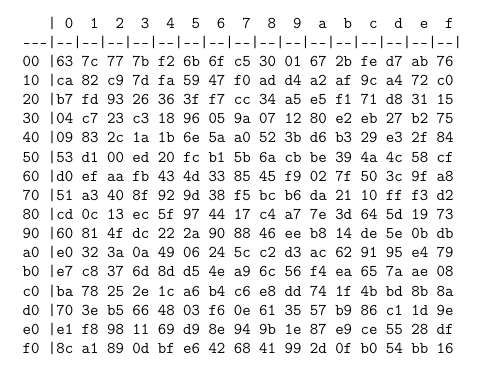
\includegraphics[scale=0.95]{subbytes}
% \end{center}
%  \caption{Tabellierung von \texttt{SubBytes}.}\label{fig:subbytes}
% \end{figure}
% 
% Die Transformation \texttt{SubBytes} wendet die Abbildung $s$ buchstabenweise an:
% \[\texttt{SubBytes}(p_1, \dots, p_{16}) = (\sigma(p_1), \dotsc, \sigma(p_{16}))\]
% für alle $(p_1, \dots, p_{16}) \in \GF(2^8)^{16} = \mc P = \mc C$.
% 
% Mit Abbildung \ref{fig:subbytes} kann beispielsweise
% \begin{align*}
% \texttt{SubBytes(}&\texttt{32 43 f6 a8 88 5a 30 8d 31 31 98 a2 e0 37 07 34)} \\
%  =\;\;& \texttt{23 1a 42 c2 c4 be 04 5d c7 c7 46 3a e1 9a c5 18}
% \end{align*}
% berechnet werden.
% 
% \subsubsection{Die Transformation \texttt{ShiftRows}}
% 
% Die Transformation \texttt{ShiftRows} permutiert die Buchstaben eines Blocks $p = (p_1, \dots, p_{16}) \in \GF(2^8)^{16}$ wie folgt:
% \[\texttt{SubBytes}(p) = (p_1, p_6, p_{11}, p_{16}, p_5, p_{10}, p_{15}, p_4, p_9, p_{14}, p_3, p_8, p_{13}, p_2, p_7, p_{12})\]
% Die Permutation \texttt{ShiftRows} bildet für alle $i=1, \dotsc, 16$ den $i$-ten Buchstaben auf den $(5⋅ i)$-ten Buchstaben modulo $16$ ab.
% 
% Beispielsweise gilt:
% \begin{align*}
% 	           &\texttt{01 02 03 04 05 06 07 08 09 10 11 12 13 14 15 16}  \\
% \texttt{ShiftRows(}&\texttt{23 1a 42 c2 c4 be 04 5d c7 c7 46 3a e1 9a c5 18)}\\
%  =\;\;& \texttt{23 be 46 18 c4 c7 c5 c2 c7 9a 42 5d e1 1a 04 3a}
% \end{align*}
% 
% \subsubsection{Die Transformation \texttt{MixColumns}}
% 
% Die Transformation \texttt{MixColumns} operiert auf Blöcken der Länge $4$, also auf $\GF(2^8)^4$. Wir definieren die lineare Abbildung
% \[S: \GF(2^8)^4 → \GF(2^8)^4, \;\; \begin{pmatrix}
%                                               p_1 \\
%                                               p_2 \\
%                                               p_3 \\
%                                               p_4 
%                                              \end{pmatrix}
%  ↦ \begin{pmatrix}
%               \texttt{02} & \texttt{03} & \texttt{01} & \texttt{01} \\
%               \texttt{01} & \texttt{02} & \texttt{03} & \texttt{01} \\
%               \texttt{01} & \texttt{01} & \texttt{02} & \texttt{03} \\
%               \texttt{03} & \texttt{01} & \texttt{01} & \texttt{02}
%              \end{pmatrix} 
%              \begin{pmatrix}
%               p_1 \\
%               p_2 \\
%               p_3 \\
%               p_4
%              \end{pmatrix}.
% \]
% % mit der Matrix
% % \[ B = \begin{pmatrix}
% %               \texttt{02} & \texttt{03} & \texttt{01} & \texttt{01} \\
% %               \texttt{01} & \texttt{02} & \texttt{03} & \texttt{01} \\
% %               \texttt{01} & \texttt{01} & \texttt{02} & \texttt{03} \\
% %               \texttt{03} & \texttt{01} & \texttt{01} & \texttt{02}
% %              \end{pmatrix} \in \GF(2^8)^{4 × 4}.\] 
% Die Einträge der Matrix sind Hexadezimalzahlen. Diese stehen für die entsprechnenden Vektoren $(a_0, \dotsc, a_7) \in \Z_2^8$ und diese wiederum für die Restklasse 
% \[a_0 + \dotsc + a_7t^7 + (f_{AES}) \in \Z_2[t]/(f) = \GF(2^8).\]
% 
% 
% Es gilt beispielsweise
% \begin{align*}
% S(\texttt{23 be 46 18}) =&  \begin{pmatrix}
%               \texttt{02} & \texttt{03} & \texttt{01} & \texttt{01} \\
%               \texttt{01} & \texttt{02} & \texttt{03} & \texttt{01} \\
%               \texttt{01} & \texttt{01} & \texttt{02} & \texttt{03} \\
%               \texttt{03} & \texttt{01} & \texttt{01} & \texttt{02}
%              \end{pmatrix} 
%              \begin{pmatrix}
%               \texttt{23} \\
%               \texttt{b6} \\
%               \texttt{46} \\
%               \texttt{18}
%              \end{pmatrix} \\
%              =&\begin{pmatrix}
%                 \texttt{02 * 23 + 03 * b6 + 01 * 46 + 01 * 18} \\
%                 \texttt{01 * 23 + 02 * b6 + 03 * 46 + 01 * 18} \\
%                 \texttt{01 * 23 + 01 * b6 + 02 * 46 + 03 * 18} \\
%                 \texttt{03 * 23 + 01 * b6 + 01 * 46 + 02 * 18} 
%                \end{pmatrix} \\
%               =&\begin{pmatrix}
%                 \texttt{02 * 23 + 03 * b6 +  46 + 18} \\
%                 \texttt{23 + 02 * b6 + 03 * 46 +  18} \\
%                 \texttt{23 + b6 + 02 * 46 + 03 * 18} \\
%                 \texttt{03 * 23 + b6 + 46 + 02 * 18} 
%                \end{pmatrix}
% \end{align*}
% 
% Wie berechnen wir nun beispielsweise \texttt{03*b6}? Diese beiden Hexadezimalzahlen entsprechen den Restklassen $t + \ol 1 + (f_{AES})$ und $t^7 + t^5 + t^4 + t^2 + t + (f_{AES})$ in $\Z_2[t]/(f_{AES})$. Das Produkt der beiden Restklassen ist 
% \[t^8 + t^7 +t^6 + 2t^5 + t^4 + t^3 + 2t^2 + t + (f_{AES}) = t^8 + t^7 +t^6 + t^4 + t^3 + t + (f_{AES}).\]
% Mit Polynomdivision in $\Z_2[t]$ durch $f_{AES}$ erhalten wir 
% \[t^8 + t^7 +t^6 + t^4 + t^3 + t = f_{AES} + t^7 + t^6 + 1\]
% \[t^8 + t^7 +t^6 + t^4 + t^3 + t + (f_{AES}) = t^7 + t^6 + 1 + (f_{AES}).\]
% Diese Restklasse entspricht \texttt{c1} in der Hexadezimaldarstellung.
% \begin{align*}
% S(\texttt{23 be 46 18}) =& \begin{pmatrix}
%                 \texttt{02 * 23 + 03 * b6 +  46 + 18} \\
%                 \texttt{23 + 02 * b6 + 03 * 46 +  18} \\
%                 \texttt{23 + b6 + 02 * 46 + 03 * 18} \\
%                 \texttt{03 * 23 + b6 + 46 + 02 * 18} 
%                \end{pmatrix} \\
%                =&\begin{pmatrix}
%                 \texttt{46 + c1 +  46 + 18} \\
%                 \texttt{23 + 67 + cc +  18} \\
%                 \texttt{23 + b6 + 88 + 24} \\
%                 \texttt{89 + b6 + 46 + 30} \\ 
%                \end{pmatrix} \\
%                 =&\begin{pmatrix}
%                 \texttt{55} \\
%                 \texttt{04} \\
%                 \texttt{69} \\
%                 \texttt{99} \\ 
%                \end{pmatrix}
% \end{align*}
% 
% Die Additionen werden analog zur oben beschriebenen Multiplikation durchgeführt.
% 
% Die Transformation \texttt{MixColumns} wendet die lineare Abbildung $S$ blockweise an:
% \[\texttt{MixColumns}(p) = \(S(p_1, p_2, p_3, p_4), S(p_5, p_6, p_7, p_8), S(p_9, p_{10}, p_{11}, p_{12}), S(p_{13}, p_{14}, p_{15}, p_{16})\)\]
% für alle $(p_1, \dots, p_{16}) \in \GF(2^8)^{16} = \mc P = \mc C$.
% \begin{exercise}
%  Berechnen Sie im Hexadezimalsystem und in $\Z_2[t]/(f_{AES})$:
%  \begin{enumerate}
%   \item \texttt{06 + ca}, \texttt{4e + b3}
%   \item \texttt{06 * ca}, \texttt{4e * b3}
%  \end{enumerate}
% \end{exercise}
% 
% \begin{exercise}
%  Geben Sie den Entschlüsselungsalgorithmus von AES in Pseudocode an.
% \end{exercise}

% 
% \section{Pseudozufallszahlen}
% 
% Um Nachrichten in Secret"=Key"=Kryptosystemen, beispielsweise AES, sicher übertragen zu können, müssen Schlüssel gewählt werden. Die Sicherheit eines Kryptosystems ist nur dann gewährleistet, wenn alle Schlüssel $k \in \mc K$ mit derselben Wahrscheinlichkeit erzeugt werden -- ansonsten würde der Schlüsselraum \enquote{schrumpfen}. Ist die Schlüsselmenge $\Z_2^{128}$, wie in der vorgestellten Version von AES, so muss eine zufällige Folge von Nullen und Einsen der Länge $128$ erzeugt werden. Ein Programm oder Gerät, das dies leistet, wird \emph{Zufallsbit-Generator} genannt. 
% 
% Folgen von Zufallsbits können mittels Hardware oder Software erzeugt werden. Hardware-Zufallsbit-Generatoren nutzen beispielsweise die Zufälligkeit des radioaktiven Zerfalls, die Zufälligkeit des Münzwurfs oder das zufällige Rauschen elektronischer Bauteile, Software-Zufallsbit-Generatoren die verstrichene Zeit zwischen zwei Anschlägen der Tastatur.
% 
% Da die Erzeugung von Zufallsbits aufwändig ist, werden in der Kryptographie andere Verfahren zur Schlüsselerzeugung genutzt, sogenannte Pseudozufallsbit-Generatoren. Diese benötigen als Eingabe eine kurze Folge von Zufallsbits und erzeugen daraus eine längere Bitfolge. Kryptographisch sichere Pseudozufallsbit-Generatoren zeichnen sich dadurch aus, dass die erzeugten Bitfolgen in der Praxis nicht von echten Zufallsbitfolgen zu unterscheiden sind. Was \enquote{in der Praxis} bedeutet, darauf gehen wir nun genauer ein.
% 
% \begin{definition}[Polynomieller Algorithmus]
%  \begin{enumerate}
%   \item Sei $n \in \N$ eine Zahl. Dann bezeichnen wir mit $\size(n)$ die Anzahl der Ziffern in ihrer Binärdarstellung. Beipielsweise ist $49$ in Binärdarstellung $110001$ und $\size(49) = 6$.
%   \item Sei $A$ ein Algorithmus, der natürliche Zahlen $z_1, \dots, z_n \in \N$ als Input hat. Wir nennen $A$ \emphex[Algorithmus!polynomiell]{polynomiell}, wenn die Laufzeit $L_A(z_1, \dotsc, z_n)$ von $A(z_1, \dotsc, z_n)$ durch ein Polynom in der \emphex{Eingabebröße} $\size(z_1), \dots, \size(z_n)$ beschränkt ist. Genauer:
% 
%  Es existieren $C > 0$, $z_1^0, \dots, z_n^0 \in \N$ und $e_1, \dots, e_n \in \N$, so dass für alle $z_1 > z_1^0, \dotsc, z_n > z_n^0$ gilt:
%  \[L_A(z_1, \dotsc, z_n) \leq C \cdot \size(z_1)^{e_1} \cdot \dotsc \cdot \size(z_n)^{e_n}.\]
%  \end{enumerate}
% \end{definition}
% 
%  Probleme, die mithilfe eines polynomiellen Algorithmus gelöst werden können, werden als \emphex{praktisch lösbar} betrachtet. Das liegt an folgendem Sachverhalt: Wenn die Eingabegröße eines Algorithmus (sprich: die Zahlen, die er als Eingabe erhält) wächst, steigt in der Regel auch die Laufzeit des Algorithmus. Für nicht-polynomielle Algorithmen steigt die Laufzeit deutlich schneller an, als die Eingabegröße wächst. Dadurch kann es passieren, dass ein Problem bereits bei einer Verdoppelung der Eingabegröße nicht mehr in vertretbarer Zeit gelöst werden kann. Bei polynomiellen Algorithmen passiert so etwas (in der Regel) nicht. Liegt kein polynomieller Lösungsalgorithmus vor, wird ein Problem als \emph{praktisch unlösbar} betrachtet, auch wenn man theoretisch weiß, wie es gelöst werden könnte. 
%  
% \begin{notation}
%     Sei $(\Omega, P)$ ein Wahrscheinlichkeitsraum. Für $k \in \N$ bezeichnen wir mit $U_k: \Omega → \{0, 1\}^k$ die gleichverteilte Zufallsvariable auf $(\Omega, P)$. (Für unsere Zwecke ist es egal, was $\Omega$ und $P$ tatsächlich sind.)
% \end{notation}
%   
%  \subsection{Pseudozufallsbit-Generatoren}
% 
%   \begin{definition}[Pseudozufallsbit-Generator]
%    Ein polynomieller deterministischer Algorithmus $G: \{0, 1\}^* → \{0, 1\}^*$ heißt \emphex[Pseudozufallsbit-Generator]{Pseudozufallsbit-Generator (PRBG)} (engl.: pseudo-random bit generator), wenn eine Funktion $n: \N → \N$ existiert, die $n(k) > k$ und $G(\{0, 1\}^k \subset \{0, 1\}^{n(k)}$ für alle $k \in \N$ erfüllt. Die Funktion $n$ heißt \emphex[Stretchfunktion]{Stretchfunktion von $G$}.
%    
%   \end{definition}
% 
%    Wir gehen nun der Frage nach, wie man die Güte eines Pseudozufallsbit-Generators bewerten kann. Von einem guten Generator würde man erwarten, dass die Verteilung der erzeugten Bitfolgen nicht von einer Gleichverteilung zu unterscheiden ist. Diese Idee fassen wir nun formaler. 
%    
%    
%    \begin{definition}[Statistischer Test]
%     Ein statistischer Test ist ein polynomieller probabilistischer Algorithmus 
%    \[A: \{0, 1\}^* → \{0, 1\}, \; \; s ↦ A(s).\]
%    Man sagt, dass $s \in \{0, 1\}^*$ den Test $A$ besteht, falls $A(s) = 1$ gilt.
%    \end{definition}
% 
%   
%    Mithilfe statistischer Tests können wir die Güte eines Pseudozufallsbit-Generators testen. Für jeden statistischen Test $A$ muss ein \emph{guter} Pseudozufallsbit-Generator Folgendes leisten: Statistisch lassen sich die Ergebnisse des Tests $A$ bei gleichverteilter Eingabe nicht von den Ergebnissen von $A \circ G$ unter gleichverteilter Eingabe unterscheiden.
% 
% \begin{figure}
% \begin{center}
%     \begin{tikzpicture}
%      \node (0) at (-2, 2) {};
%      \node (*) at (-2, 0) {$\{0, 1\}^*$};
%      \node (01) at (-2, -2) {$\{0, 1\}$};
%      \node (0r) at (2, 2) {};
%      \node (*r) at (2, 0) {$\{0, 1\}^*$};
%      \node (01r) at (2, -2) {$\{0, 1\}$};
%      \draw[-latex] (0) -- node [left] {$U_k$} (*); 
%      \draw[-latex] (*) -- node [left] {$A$} (01);
%      \draw[-latex] (*) -- node [above] {$G$} (*r);
%      \draw[-latex] (*r) -- node [right] {$A$} (01r);
%     \end{tikzpicture}
%    \end{center}
%    \caption{Statistischer Test $A$ eines Pseudozufallsbit-Generators $G$. Dabei ist $U_k$ ist die gleichverteilte Zufallsvariable auf $\{0, 1\}^k$.}\label{fig:testprbg}
%    \end{figure}
%    Ansonsten würde nämlich ein (polynomieller) statistischer Test, also ein in der Praxis anwendbarer Test existieren, durch den man herausfinden kann, dass sich der Output des Pseudozufallsbit-Generators $G$ anders verhält als der Input von $G$, siehe auch Abbildung \ref{fig:testprbg}
%    
%    Wie können wir testen, ob $G$ diese Eigenschaft erfüllt? Dazu betrachten wir die Zufallsvariablen $A \circ U_k$ und $A \circ G \circ U_k$. Nun gibt $P_{A \circ U_k}(1)$ die Wahrscheinlichkeit dafür an, dass ein gemäß der Gleichverteilung $U_k$ gewähltes $s \in \{0, 1\}^k$ den Text $A$ besteht. Analog gibt $P_{A \circ G \circ U_k}(1)$ die Wahrscheinlichkeit an, dass ein gemäß der Gleichverteilung $U_k$ gewähltes $s \in \{0, 1\}^k$ den Test $A$ besteht. Bei einem \emph{guten} Pseudozufallsbit-Generator sollten diese beiden Wahrscheinlichkeiten nicht zu unterscheiden sein.
%   
%   Diese Überlegung führt uns zu den folgenden Definitionen.
%     
%   \begin{definition}[Vernachlässigbare Funktion]
%    Eine Funktion $f: \N → \R$ heißt \emphex{vernachlässigbar}, wenn für jedes Polynom $g$ mit $\lim\limits_{k → \infty} g(k) = \infty$ ein $k_0 \in \N$ existiert, so dass für alle $k \geq k_0$ gilt:
%  \[|f(k)| < \frac{1}{g(k)},\]
%  d.\,h. $f$ \enquote{fällt schneller} als $k ↦ \frac{1}{g(k)}$.
%   \end{definition}
% 
% Das wohl prominenteste Beispiel für eine vernachlässigbare Funktion ist $k ↦ \exp(-k)$.   
%   
%  
%   \begin{definition}[Kryptographisch sicherer Pseudozufallsbit-Generator (CSPSBG)]
%   Es sei $G$ ein Pseudozufallsbit-Generator mit Stretchfunktion $n$ und $A$ ein statistischer Test.
%   \begin{enumerate}
%  \item Wir sagen, dass $G$ den Test $A$ \emph{besteht}, wenn
%  \[\N → \R, \;\; k ↦ P_{A \circ G \circ U_k}(1) - P_{A \circ U_{n(k)}}(1)\]
%  vernachlässigbar ist.
%  \item Wir nennen $G$ \emphex[Pseudozufallsbit-Generator!kryptographisch sicher]{kryptographisch sicher (CSPRBG)}, wenn $G$ alle polynomiellen statistischen Tests besteht.
%   \end{enumerate}
%  \end{definition}  
%  
%   Anschaulich ist ein Pseudozufallsbit-Generator $G$ genau dann kryptographisch sicher, wenn kein polyonieller statistischer Test $A$ existiert, also kein in der Praxis durchführbarer Test, für den man die Ergebnisse von $A \circ G$ von denen von $A$ unterscheiden kann. 
%   
%   Nun können wir einen Pseudozufallsbit-Generator schwerlich \emph{allen} statistischen Tests unterziehen, um herauszufinden, ob er kryptographisch sicher ist. Ein wenig einfacher wird es durch den Satz von Yao, der uns sagt, dass wir uns auf sogenannte \emph{Next-Bit-Tests} beschränken können.
%   
%   \begin{definition}[Next-Bit-Test]
%    \begin{enumerate}
%     \item Sei $B: \{0, 1\}^* → \{0, 1\}$ durch einen polynomiellen Algorithmus gegeben. Der \emphex[Next-Bit-Test]{Next-Bit-Test mit Vorhersage $B$} ist der statistische Test $A_B$, der durch
%   \[A_B: \{0, 1\}^* → \{0, 1\}, \; \; s = (s_0, \dots, s_k) ↦ A_B(s) = \begin{cases}
%                                                                                        0 &\text{falls } B(s_0, \dotsc, s_{k-1}) = s_k\\
%                                                                                        1 & \text{falls } B(s_0, \dotsc, s_{k-1}) ≠ s_k
%                                                                                       \end{cases}\]
% definiert ist, d.\,h. $A_B(s)$ ist $0$, wenn $B$ das letzte Bit von $s$ korrekt vorhergesagt hat, und $1$, wenn das letzte Bit falsch vorhergesagt wurde.
% \item  Wir nennen einen Pseudozufallsbit-Generator $G$ \emphex[Pseudozufallsbit-Generator!unvorhersagbar]{unvorhersagbar}, wenn $G$ alle Next-Bit-Tests besteht.
%    \end{enumerate}
%   \end{definition}
% 
%  \begin{remark}\label{rem:half}
%   Da $B$ polynomiell ist, ist auch $A_B$ polynomiell. Außerdem gilt für die gleichverteilte Zufallsvarible $U_k: \Omega → \{0, 1\}^k$ unabhängig von $B$
%   \[P_{A_B \circ U_k}(1) = P_{A_B \circ U_k}(0) = \frac 1 2:\]
%   Da das letzte Bit eines unter der Gleichverteilung gewählten $(s_0, \dots, s_n) \in \{0, 1\}^*$ nicht von den vorherigen Bits abhängt, wird die Vorhersage $s_n = B(s_0, \dots, s_{n-1})$ unabhängig von $B$ in genau der Hälfte der Fälle korrekt sein. 
%  \end{remark}
%   
%  
%  \begin{theorem}[Yao]
%   Ein Pseudozufallsbit-Generator ist genau dann kryptographisch sicher, wenn er unverhersagbar ist.
%  \end{theorem}
% 
% \subsection{Beweisbare Sicherheit}
% 
% \todo{Beweise pimpen}
% 
% Als nächstes werden wir Pseudozufallsbit-Generatoren konstruieren, von denen (unter Standardannahmen) bewiesen werden kann, dass sie unverhersagbar und somit, mit dem Satz von Yao, kryptographisch sicher sind. 
% 
% \begin{notation}
%  Seien $f: \{0, 1\}^* → \{0, 1\}^*$ eine Funktion und $A:\{0, 1\}^* → \{0,1\}^*$ ein probabilistischer Algorithmus. Dann definieren wir den statistischen Test
%  \[A_f: \{0, 1\}^* → \{0, 1\}, \; \; \; x ↦ \begin{cases}
%                                                              1 & \text{falls } f(A(f(x)) = x, \\
%                                                              0 & \text{sonst.}
%                                                             \end{cases}\]
%   Es gilt genau dann $f(A(f(x)) = x$, wenn $A(f(x))$ ein Urbild von $f(x)$ ist; die Funktion $A_f$ testet also, für welche $x \in \{0, 1\}^*$ der Algorithmus $A$ ein Urbild berechnet.
%   
%   Die Funktion $A_f \circ U_k$ ist eine Zufallsvaribale auf $(\Omega, P)$.
% \end{notation}
% 
% \begin{definition}[Einwegfunktion]
%  \begin{enumerate}
%   \item Sei $f: \{0, 1\}^* → \{0, 1\}^*$ ein polynomieller deterministischer Algorithmus. Dann heißt $f$ \emphex[Einwegfunktion]{Einwegfunktion (EF)}, wenn
%   \[k ↦ P_{A_f \circ U_k}(1)\]
%   für jeden probabilistischen Algorithmus $A: \{0, 1\}^* → \{0, 1\}^*$ vernachlässigbar ist.
%   \item Eine Einwegfunktion $f$ heißt \emphex[Einwegpermutation]{Einwegpermutation (EP)}, falls sie bijektiv ist und Längen erhält, d.\,h. $f(\{0, 1\}^n) = \{0, 1\}^n$ für alle $n \in \N$.
%   \end{enumerate}
% \end{definition}
% 
% In der Definition von Einwegfunktion steht $P_{A_f \circ U_k}(1)$ für die Wahrscheinlichkeit, dass $$f(A(f(x)))= x$$ gilt, also dass der Algorithmus $A$ ein Urbild von $x \in \{0, 1\}^k$ unter $f$ findet. Anschaulich gesprochen ist ein deterministischer Algorithmus $f$ also eine Einwegfunktion, wenn $f(x)$ \enquote{leicht}, sprich in polynomieller Zeit zu berechnen ist und wenn die Wahrscheinlichkeit, dass $A$ ein Urbild von $f(x)$ unter $f$ findet, für jeden polynomiellen Algorithmus $A$ vernachlässigbar ist. Obwohl die Berechnung von $f(x)$ kein Problem darstellt, ist es \enquote{praktisch unmöglich} ein Urbild von $f(x)$ unter der Einwegfunktion $f$ zu finden.
% 
% \begin{definition}[Sicherheitsbit]
%  Sei $f: \{0, 1\}^* → \{0, 1\}^*$ ein polynomieller deterministischer Algorithmus. 
%  \begin{enumerate}
%   \item Für einen polynomiellen deterministischen Algorithmus $b:\{0, 1\}^* → \{0, 1\}$ und einen statistischen Test $A$ definieren wir
%   \[A_{f, b}: \{0, 1\}^* → \{0, 1\}, \;\; x ↦ \begin{cases}
%                                                                1 & \text{falls } A(f(x)) = b(x),\\
%                                                                0 & \text{sonst.}
%                                                               \end{cases}\]
%   \item $b$ heißt \emphex[Sicherheitsbit]{Sicherheitsbit für $f$}, wenn 
%   \[\N → \R, \;\; k ↦ P_{A_{f, b} \circ U_k}(1) - \frac 1 2\]
%   für alle statistischen Tests $A$ vernachlässigbar ist.
%  \end{enumerate}
% \end{definition}
% 
% 
% \begin{remark}
% Ein Sicherheitsbit zeigt in konzentrierter Weise an, dass es schwer ist ein Urbild von $f(x)$ unter $f$ zu berechnen:
% 
% Wenn $b$ ein Sicherheitsbit für $f$ ist, dann geht die Wahrscheinlichkeit, dass ein polynomieller Algorithmus $A$ aus $f(x)$ das Bit $A(f(x)) = b(x)$ berechnet, gegen $\frac 1 2$, d.\,h. es gibt keinen polynomiellen Algorithmus, der $b(x)$ aus der Kenntnis von $f(x)$ besser als durch Raten bestimmen kann. 
% \end{remark}
% 
% \begin{lemma}
%  Sei $f: \{0, 1\}^* → \{0, 1\}^*$ ein polynomieller deterministischer Algorithmus, der injektiv ist, und sei $b$ ein Sicherheitsbit für $f$. Dann ist $f$ eine Einwegfunktion.
% \end{lemma}
% \begin{proof}
%  Angenommen es gäbe einen Algorithmus $A$, so dass $f$ den statistischen Test $A_f$ nicht besteht. Dann ist $k ↦ P_{A_f \circ U_k}(1)$ nicht vernachlässigbar. Wir definieren $A' = b \circ A$. Dann ist auch $k ↦ P_{A'_{f, b} \circ U_k}(1) - \frac 1 2$ nicht vernachlässigbar, d.\,h. $A'$ kann $b(x)$ aus $f(x)$ besser bestimmen als mit Wahrscheinlichkeit $\frac 1 2$. 
% \end{proof}
% 
% \begin{theorem}\label{thm:csprbg}
%  Es seien $f$ eine Einwegpermutation mit Sicherheitsbit $b$ und $n: \N → \N$ eine beliebige Funktion, die $n(k) > k$ für alle $k \in \N$ erfüllt und die durch einen polynomiellen Algorthmus berechnet werden kann. Dann ist 
%  \[G: \{0, 1\}^* → \{0, 1\}^*, \; \; s=(s_1, \dots, s_k) ↦ \(b(s), b(f(s)), \dotsc, b\(f^{n(k)-1}(s)\)\)\]
%  ein kryptographisch sicherer Pseudozufallsbit-Generator.
% \end{theorem}
% \begin{proof}
%  Es sei $G'$ der Pseudozufallsbit-Generator, der durch
%  \[s ↦ \(f^{n(k) -1}(s), \dotsc , b(f(s)), b(s)\)\]
%  definiert ist. Da die kryptographische Sicherheit eines Pseudozufallsbit-Generators nicht von der Reihenfolge der Bits im Output abhängt, ist $G$ genau dann kryptographisch sicher, wenn $G'$ es ist. 
%  
%  Wir nehmen nun an, dass $G'$ nicht kryptographisch sicher ist. Mit dem Satz von Yao existiert dann ein Next-Bit-Text $A_B$, den $G'$ nicht besteht. Es gibt also einen polynomiellen deterministischen Algorithmus $B$, der $b(s)$ aus der Kenntnis von $\(f^{n(k) -1}(s), \dotsc , b(f(s))\)$ statistsch vorhersagen kann. Präziser: es gilt, dass die Funktion 
%  \[k ↦ P_{A_B \circ U_k}(1) - P_{A_B \circ G' \circ U_k}(1) = \frac 1 2 - P_{A_B \circ G' \circ U_k}(1)\]
%  (siehe Bemerkung \ref{rem:half}) nicht vernachlässigbar ist. Die Funktion $A_B \circ G'$ ist dabei gegeben durch
%  \[(s_0, \dots s_k) ↦ \begin{cases}
%                              1 & \text{falls } B(b(f^{n(k)-1}(s)), \dotsc, b(f(s))) = b(s),\\
%                              0 & \text{sonst.}
%                             \end{cases}\]
%  Wir defineren die Funktion $A: \{0, 1\}^* → \{0, 1\}$ durch
%  \[s ↦ B(b(f^{n(k)-2}(s)), \dotsc, b(s))\]
%  Dann gilt $A(f(s)) = B(b(f^{n(k)-1}(s)), \dotsc, b(f(s)))$ für alle $s \in \{0, 1\}^k$ und $A_B \circ G' = A_{f, b}$. 
%  Folglich ist 
%  \[k ↦ \frac 1 2 - P_{A_{f, b} \circ U_k}(1)\]
%  nicht vernachlässigbar -- im Widerspruch dazu, dass $b$ ein Sicherheitsbit für $f$ ist. 
% \end{proof}
% 
% 
% 
% \subsection{Kandidaten für Einwegfunktionen}
% 
% Unter der Annahme, dass eine Einwegfunktion existiert und bekannt ist, können wir mit \ref{thm:csprbg} kryptographisch sichere Pseudozufallsbit-Generatoren konstruieren. Auch wenn es Kandidaten für solche Einwegfunktionen gibt, konnte ihre Existenz bis heute nicht bewiesen werden. Man kann sogar zeigen, dass Einwegfunktionen genau dann existieren, wenn die Komplexistätsklassen P und NP verschieden sind. Die Fragestellung, ob P = NP gilt, ist eins der sieben Millenium-Probleme, für deren Lösung das Clay Mathematics Institute im Jahr $2000$ jeweils eine Million US-Dollar ausgelobt hat. Bisher konnte erst eins der Probleme gelöst werden, durch den Beweis der sogenannten Poincaré-Vermutung im Jahr 2002 durch den russischen Mathematiker Grigori Jakowlewitsch Perelman.
% 
%  \begin{definition}[Komplexitätsklassen]
%   Ein Problem $\Pi$ liegt in der Komplexitätsklasse
%   \begin{itemize} 
%   \item P, wenn $\Pi$ durch einen polynomiellen deterministischen Algorithmus gelöst werden kann.
%    \item BPP, wenn $\Pi$ durch einen polynomiellen probabilistischen Algorithmus gelöst werden kann, dessen Fehlerwahrscheinlichkeit höchstens $\frac 1 3$ ist. (Die Schranke $s = \frac 1 3$ ist dabei willkürlich mit $\frac 1 2 < s < 1$ gewählt.)
%   \end{itemize}
%  \end{definition}
% 
% \begin{construction}[Kandidaten für Einwegfunktionen]
% \begin{enumerate}
%  \item \emphex[Faktorisierungsproblem]{Das Faktorisierungsproblem (FP)}: Sei $n \in \N$. Finde eine Primzahl $p \in \N$, die $n$ teilt.
%  \item \emphex[Logarithmus-Problem!diskrete]{Das diskrete Logarithmus-Problem (DLP)}: Sei $G = \langle g \rangle = \{g^0, g^1, g^2, \dotsc\}$ eine endliche zyklische Gruppe der Ordnung $n \in \N$ und $x \in G$. Finde ein $a \in \N$, so dass $g^a = x$ gilt. 
% %  \item \emphex[Diffie-Hellman-Problem]{Das Diffie-Hellman-Problem (DHP)}: Seien $G = \langle g \rangle$ eine endliche zyklische Gruppe und $A, B \in \N$. Gegeben $g$, $g^A$ und $g^B$, berechne $g^{A \cdot B}$.
% %  \item \emphex[RSA-Problem]{Das RSA-Problem (RSAP)}:
% \end{enumerate}
% (Frage: Was ist jeweils die Eingabegröße der Probleme?)
% \end{construction}
% 
% Von keinem dieser Probleme ist bekannt, ob sie in der Komplexitätsklasse BPP liegen. Dennoch trifft man in der Kryptogrphie folgende Standardannahmen. Nur unter solchen Annahmen kann die Existenz kryptographisch wertvoller Einwegfunktionen bewiesen werden. 
% 
% \begin{assumption}
%  \begin{itemize}
%   \item \emphex[Fakorisierungsannahme]{Faktorisierungs-Annahme (FA)}: Das Faktorisierungsproblem liegt \textbf{nicht} in der Komplexitätsklasse BPP. 
%   \item \emphex[Logarithmus-Annahme]{Logarithmus-Annahme (LA)}: Das diskrete Logarithmus-Problem liegt \textbf{nicht} in der Komplexitätsklasse BPP.
% %   \item Diffie-Hellman-Annahme: Das Diffie-Hellman-Problem liegt \textbf{nicht} in der Komplexitätsklasse BPP.
%  \end{itemize}
% \end{assumption}
% 
% \begin{example}
%  Sei $p \in \N$ eine Primzahl und $a \in \Z_p$ eine Primitivwurzel, d.\,h. $\langle a \rangle = \Z_p$. Unter der Logarithmus-Annahme ist
%  \[f: \{1, \dots, p-1\} → x ↦ a^x \mod p\]
%  eine Einwegfunktion mit Sicherheitsbit
%  \[b(x) = \begin{cases}
%            1 & \text{falls } x < \frac p 2,\\
%            0 & \text{falls } x \geq \frac p 2. \\
%           \end{cases}\]
% \todo{Wieso?}
% Für jede Stretchfunktion $n: \N → \N$ ist mit Satz \ref{thm:csprbg} 
% \[G: \{0, 1\}^* → \{0, 1\}^*, \;\; s = (s_0, \dots, s_n) ↦ (b(f^{n(k)-1}(s)), \dots, b(s))\]
% ein kryptographisch sicherer Pseudozufallsbit-Generator.
% \end{example}


\chapter{Public"=Key"=Kryptosysteme}

Bei der Verwendung von Secret"=Key"=Kryptosystemen zur Verschlüsselung von Botschaften kennen sowohl Sender als auch Empfänger den geheimen Verschlüsselungsschlüssel $e \in \mc K$, mit dem ein Klartext $p \in \mc P$ zu einem Chiffretext $c = E_e(p)$ verschlüsselt wird. Dieser geheime Schlüssel $e$ muss vor seiner Verwendung bei einem Treffen zwischen Sender und Empfänger ausgetauscht werden. Aus dem Verschlüsselungsschlüssel $e$ können beide \enquote{leicht} einen zugehörigen Entschlüsselungsschlüssel $d(e) \in \mc K$ berechnen und den Chiffretext $c$ zu $D_{d(e)}(c)= p$ entschlüsseln. Verschlüsselung mittels Secret"=Key"=Kryptosystemen hat somit den Nachteil, dass der geheime Schlüssel $e$ irgendwann vor der Kommunikation ausgetauscht worden sein muss; anders ausgedrückt: Es muss ein Treffen zwischen Sender und Empfänger stattgefunden haben.

In Public-Key-Kryptosystemen ist das anders. Hier können verschlüsselte Nachrichten übermittelt werden, ohne dass vorher ein Austausch eines geheimen Schlüssels zwischen Sender und Empfänger stattgefunden hat. Der Austausch eines geheimen Schlüssels wird überflüssig, da bei Public-Key-Kryptosystemen der Verschlüsselungsschlüssel $e \in \mc K$ öffentlich, das heißt frei zugänglich ist -- daher der Name \enquote{Public-Key}. Da jeder Zugriff auf den Verschlüsselungsschlüssel $e \in \mc K$ hat, kann jeder beliebige Botschaften $p \in \mc P$ zu Chiffretexten $c = E_e(p)$ verschlüsseln. 

Dieses Wissen um den Verschlüsselungsschlüssel stärkt die Position eines Angreifers: Ein Angreifer fängt den Chiffretext $c = E_e(p) \in \mc C$ ab, kennt den genutzten Verschlüsselungsschlüssel $e$ und kann beliebige Klartexte $p \in \mc P$ verschlüsseln. Bei Public-Key-Kryptosystemen stehen einem Angreifer somit alle Zutaten für einen Chosen-Plaintext-Angriff zur Verfügung.

Diesen \enquote{Nachteil} machen Public-Key-Kryptosysteme durch eine andere Eigenschaft wett: In Public-Key-Systemen ist es \enquote{unzulässig} aus der Kenntnis des Verschlüsselungsschlüssels $e$ den zugehörigen Entschlüsselungsschlüssel $d(e)$ zu berechnen, d.\,h.: Die Berechnung von $d(e)$ aus $e$ würde in aller Regel so lange dauern, dass die Berechnung von $d(e)$ in der Praxis unmöglich ist.

Da die Algorithmen von Secret-Key-Systemen in der Regel effizienter sind als die Algorithmen von Public-Key-Systemen, wird in der Praxis meist ein Public-Key-System genutzt, um einen geheimen Schlüssel auszutauschen. Die anschließende geheime Kommunikation erfolgt dann über ein Secret-Key-System mithilfe des bereits ausgetauschten Schlüssels.



 \subsubsection{Laufzeiten von Algorithmen}

%  \begin{definition}
%   Ein Algorithmus heißt deterministisch, wenn der Output nur vom Input abhängt. Ansonsten heißt er probabilistisch.
%  \end{definition}
% 
%  \begin{example}
%   Ein (korrekter) Algorithmus zur Addition zweier Zahlen $n, m \in \N$ ist deterministisch, er hat immer das gleiche Ergebnis $n+m \in \N$: Der Input des Algorithmus ist $(n, m) \in \N^2$, der Output immer $n + m \in \N$. 
%   
%   Ein Algorithmus, mit dem für $n \in N$ eine zufällige Zahl $0< a < n$ bestimmt wird, ist probabilistisch: Der Input des Algorithmus ist $n \in \N$, der Output kann jede Zahl $0 < a < n$ sein.
%  \end{example}
% 

 \begin{definition}[$\mc O$-Notation]
  Es sei $k \in \N$ und $f: \N^k → \R$, $g: \N^k → \R$ seien Funktionen. Man schreibt $f = \mc O(g)$, wenn positive Zahlen $C, z_1, \dots, z_k \in \N$ existieren, so dass für alle $(n_1, \dots, n_k) \in \N^k$ mit $n_i > z_i$, $1 \leq i \leq k$, Folgendes, gilt:
  \[f(n_1, \dots, n_k) \leq C \cdot g(n_1, \dots, n_k)\]
  Anschaulich heißt das, dass \enquote{fast überall} $f(n_1, \dots, n_k) \leq C \cdot g(n_1, \dots, n_k)$ erfüllt ist. Ist $g$ eine konstante Funktion, so schreibt man $f = \mc O(1)$ (da dann $f(n_1, \dots, n_k) \leq C \cdot 1$ gilt).
 \end{definition}

 \begin{example}{\ }
  \begin{itemize}
   \item $2n^2 + n + 1  = \mc O(n^2)$, da $2n^2 + n + 1 \leq 4 \cdot n^2$ für alle $n\geq1$.
   \item $3nm+ n + m +1= \mc O(nm)$, da $3mn + n + m + 1 \leq 6 \cdot mn$ für alle $n, m\geq 1$.
  \end{itemize}

 \end{example}

\begin{definition}[Polynomieller Algorithmus]{\ }
 \begin{enumerate}
  \item Sei $n \in \N$ eine Zahl. Dann bezeichnen wir mit $\size(n)$ die Anzahl der Ziffern in ihrer Binärdarstellung. (Man kann $\size(n)$ auch als $\lfloor \log_2(n) \rfloor + 1$, den abgerundeten Logarithmus von $n$ zur Basis $2$ plus $1$, beschreiben.)
  \item Sei $A$ ein Algorithmus, der natürliche Zahlen $z_1, \dots, z_n \in \N$ als Input hat. Wir nennen $A$ \emphex[Algorithmus!polynomiell]{polynomiell}, wenn $e_1, \dots, e_n \in \N$ existieren, so dass $A$ die Laufzeit
  \[\mc O\(\size(z_1)^{e_1} \cdot \dotsc \cdot \size(z_n)^{e_n}\)\]
  hat.
  \item Man sagt, dass ein Problem in der Komplexitätsklasse P liegt, wenn es durch einen polynomiellen Algorithmus gelöst werden kann.
 \end{enumerate}
\end{definition}


\begin{example}[Addition ganzer Zahlen]
 Die Addition ganzer Zahlen $n, m \in \Z$ ist in Polynomialzeit möglich, hier ein Beispiel:
 
 Seien $n = 49$, $m = 23$ mit Binärdarstellung $b_n = 110001$ und $b_m = 10111$. Dann ist $\size(n) = 6$ und $\size(m) = 5$. Um $m$ und $n$ zu addieren, müssen $6 = \max\{\size(m), \size(n)\}$ Bit-Additionen mit Übertrag durchgeführt werden:
 \begin{center}
 \begin{tabular}{rccccccc}
   & &1 & 1& 0& 0 & 0 & 1 \\
  +& &  & 1 & 0& 1 & 1 & 1\\
  Übertrag&1 & 1& & 1& 1 & 1& \\
  \hline
   & 1 &  0 &  0  & 1 & 0 & 0 & 0 
 \end{tabular}
 \end{center}
 
 
 Wir nehmen an, dass die Addition zweier Bits Zeit $\mc O(1)$, also konstante Zeit braucht. Daher braucht die gesamte Addition von $n$ und $m$ Zeit $\mc O(\max\{\size(n), \size(m)\})$. 
\end{example}

\begin{example}
 Folgende Problemstellungen können mithilfe eines polynomiellen Algorithmus gelöst werden:
 \begin{itemize}
  \item Addition ganzer Zahlen
  \item Multiplikation ganzer Zahlen
  \item Division mit Rest
  \item Erweiterter Euklidischer Algorithmus
  \item Berechnung von Inversen in $\Z_n$
 \end{itemize}
\end{example}

 Probleme, die mithilfe eines polynomiellen Algorithmus gelöst werden können, werden als \emphex{praktisch lösbar} betrachtet. Das liegt an folgendem Sachverhalt: Wenn die Eingabegröße eines Algorithmus (sprich: die Zahlen, die er als Eingabe erhält) wächst, steigt in der Regel auch die Laufzeit des Algorithmus. Für nicht-polynomielle Algorithmen steigt die Laufzeit deutlich schneller an, als die Eingabegröße wächst. Dadurch kann es passieren, dass ein Problem bereits nach einer geringen Vergrößerung der Eingabegröße nicht mehr in vertretbarer Zeit gelöst werden kann. Bei polynomiellen Algorithmen passiert so etwas (bei kleinen Exponenten $e_i$ und einer kleinen Konstante $C$) nicht. Liegt kein polynomieller Lösungsalgorithmus vor, wird ein Problem als \emph{praktisch unlösbar} betrachtet, auch wenn man theoretisch weiß, wie es gelöst werden könnte. 

 \subsubsection{Definition: Public-Key-Kryptosysteme}

 Mithilfe des Begriffs eines polynomiellen Algorithmus verfeinern wir nun die Definition eines Public-Key-Kryptosystems. 
 
\begin{definition}[Public-Key-Kryptosystem]\label{def:pkc}
 Ein \emphex{Public-Key-Kryptosystem} ist ein Kryptosystem, in dem der Schlüsselraum $\mc K = \mc K_E \dot\cup \mc K_D$ aus zwei Teilmengen besteht, dem Verschlüsselungsraum $\mc K_E$ und dem Entschlüsselungsraum $\mc K_D$, so dass folgende Eigenschaften erfüllt sind:
 \begin{enumerate}
  \item Für jeden Verschlüsselungsschlüssel $e \in \mc K_E$ existiert ein Entschlüsselungsschlüssel $d(e) \in \mc K_D$, so dass $D_{d(e)}(E_e(p)) = p$ für alle Klartexte $p \in \mc P$ gilt.
  \item Zur Auswertung aller Verschlüsselungsfunktionen $E_e \in \mc E$ und Entschlüsselungsfunktionen $D_d \in \mc D$ existieren Algorithmen mit polynomieller Laufzeit.
  \item Der genutzte Verschlüsselungsschlüssel $e \in \mc K_E$ wird veröffentlicht.
  \item Es existiert kein polynomieller Algorithmus, der aus einem Verschlüsselungsschlüssel $e \in \mc K_E$ und aus der Kenntnis des Kryptosystems den zugehörigen Entschlüsselungsschlüssel $d(e) \in \mc K_D$ berechnen kann.
 \end{enumerate}
 \end{definition}

 \begin{remark}
 In einem Public-Key-Kryptosystem existiert kein polynomieller Algorithmus, mit dem allein durch die Kenntnis eines Verschlüsselungsschlüssels $e \in \mc K_E$ der zugehörige Entschlüsselungsschlüssel $d(e) \in \mc K_D$ berechnet werden kann. Es ist also \enquote{praktisch unmöglich} $d(e)$ aus $e$ zu berechnen. Ohne die Kenntnis des Entschlüsselungsschlüssels $d(e)$ kann (in der Regel) auch ein Chiffretext $c = E_e(p) \in \mc C$ nicht in Polynomialzeit zu $p = D_{d(e)}(c) = D_{d(e)}(E_e(p)) \in \mc P$ entschlüsselt werden. 
 
 Wenn der Entschlüsselungsschlüssel $d(e)$ bekannt ist, ändert sich das: Ist $d(e)$ bekannt, kann $p = D_{d(e)}(c)$ laut Definition eines Public-Key-Kryptosystems in Polynomialzeit berechnet werden. Man sagt, dass $d(e)$ \emphex[Trapdoor-Information]{Trapdoor"=Information} enthält (engl. Falltür). Durch die Trapdoor-Information wird die Invertierung der Verschlüsselungsfunktion $E_e$ zulässig.
 \end{remark}


 
  \begin{construction}[Kommunikation mittels Public"=Key"=Kryptosystemen]
  Bob möchte geheime Nachrichten empfangen können, ohne vorher mit dem Sender der Nachricht einen geheimen Schlüssel austauschen zu müssen. Dies ist mithilfe eines Public"=Key"=Kryptosystems möglich:
  
  Bob wählt einen öffentlichen Schlüssel $e \in \mc K_E$ und einen zugehörigen geheimen Schlüssel $d(e) \in \mc K_D$. Dann veröffentlicht er den geheimen Schlüssel $e$. Nun kann Alice, die Bob bisher nicht kennt und nie getroffen hat, eine beliebige Nachricht $p \in \mc P$ zu
  \[c = E_e(p) \in \mc C\] verschlüsseln und an Bob senden. Da Bob seinen persönlichen geheimen Schlüssel $d(e)$ kennt, kann er Alices Nachricht $c$ zu \[p = D_{d(e)}(c) = D_{d(e)}(E_e(p))\] entschlüsseln. Ver- und Entschlüsselung erfolgen jeweils in Polynomialzeit.
  
  Die Sicherheit des Kryptosystems beruht darauf, dass die Berechnung von $d(e)$ aus $e$ nicht in Polynomialzeit möglich und damit \enquote{praktisch unmöglich} ist: Eine Angreiferin Eve braucht unvertretbar lange um $d(e)$ aus $e$ zu berechnen und somit (in der Regel) auch unvertretbar lange um $c$ zu $p = E_{d(e)}(c)$ zu entschlüsseln.
 \end{construction}
  
  
   \begin{remark}
   Es gibt Kryptosysteme, bei denen die Ver- oder Entschlüsselungsalgorithmen keine Funktionen, sondern sogenannte Multifunktionen sind. Ein Beispiel ist das Rabin-Kryptosystem, das im Rahmen dieser Vorlesung aus Zeitgründen jedoch nicht vorgestellt wird. Eine Multifunktion $f\colon M \multimap N$ ist eine Abbildung $\tilde f\colon M → \Pot(N)$, d.\,h.~ein Element $m \in M$ des Definitionsbereichs wird auf eine Teilmenge des Wertebereichs abgebildet.

   Ist eine Entschlüsselungsfunkion $D_d: \mc C \multimap \mc P$ eine Multifunktion, so wird ein Chiffretext $c \in \mc C$ zu einer Menge von Klartexten $D_d(c) = \{p_1, \dots, p_n\} \subset \mc P$ entschlüsselt -- und nicht nur zu einem. Um $c$ zu entschlüsseln, muss aus dieser Menge von Klartexten $\{p_1, \dots, p_n\}$ händisch der \enquote{richtige} ausgewählt werden, d.\,h.~man muss prüfen, welcher der (hoffentlich eindeutige) Klartext $p_i$ ist, der Sinn ergibt.
   \end{remark}
  
  \subsubsection{Kandidaten für Einwegfunktionen}
  
  Public-Key-Kryptosysteme bauen auf sogenannten Einwegfunktionen auf, die wir nun einführen.
  
  \begin{definition}
   Seien $k, l \in \N$. Eine Funktion $f: \N^k → \N^l$ heißt \emphex{Einwegfunktion}, wenn $f(x)$ für alle $x \in \N^k$ in Polynomialzeit berechnet werden kann und wenn gleichzeitig kein polynomieller Algorithmus existiert, der Urbilder unter $f$ berechnet.
  \end{definition}

  Anschaulich gesprochen erfüllt eine Einwegfunktion $f: \N → \N$ folgende Eigenschaft: Das Berechnen von Bildern $f(x)$ ist \enquote{einfach}, also in Polynomialzeit möglich; das Berechnen von Urbildern jedoch ist \enquote{schwierig}, also nicht in Polynomialzeit möglich, und dauert \enquote{unvertretbar lange}.
  
   \begin{remark}
  Man kann sich das Nachschlagen einer Telefonnummer in einem klassischen Papiertelefonbuch als Einwegfunktion vorstellen. Kennt man den Namen einer Person, kann man dank der alphabetischen Sortierung recht schnell und einfach herausfinden, was ihre Telefonnummer ist. Wenn man allerdings herausfinden möchte, welche Person hinter einer gegebenen Nummer steckt, muss man das gesamte Telefonbuch durchgehen, was unvertretbar lange dauert.
  \end{remark}
  

  \begin{remark}
   Bis heute ist nicht bekannt, ob Einwegfunktionen überhaupt existieren! Auch wenn es vielversprechende Kandidaten für solche Einwegfunktionen gibt, konnte ihre Existenz bis heute nicht bewiesen werden. Damit ist ebenfalls unklar, ob Public-Key-Kryptosysteme existieren: Nur unter Annahmen kann gezeigt werden, dass ein Kryptosystem die Eigenschaft erfüllt, dass der zu $e \in \mc K_E$ gehörige Entschlüsselungsschlüssel $d(e)$ nicht in Polynomialzeit bestimmt werden kann.
   
   Man kann zeigen, dass aus der Existenz von Einwegfunktionen folgen würde, dass die Komplexitätsklassen P und NP verschieden sind. P ist die Klasse der Probleme, die in polynomieller Zeit lösbar sind; NP die Klasse der Probleme, für die in polynomieller Zeit überprüft werden kann, ob ein vorgegebenes Ergebnis das Problem tatsächlich löst. 
  
   Zwei Beispiele:
   
   Das Problem der Addition zweier Zahlen $n, m \in \N$ ist, wie wir gesehen haben, in polynomieller Zeit lösbar, d.\,h.~das Ergebnis $n+m \in \N$ kann in polynomieller Zeit bestimmt werden. Dieses Problem liegt also in der Komplexitätsklasse P. Außerdem kann in polynomieller Zeit überprüft werden, ob eine Zahl $a \in \N$ die Summe von $n$ und $m$ ist, \zB indem man erst $n+m$ in polynomieller Zeit berechnet und dann überprüft, ob $a = n + m$ gilt. Damit liegt das Problem der Addition zweier Zahlen $n, m \in \N$ auch in NP. 
   
   Nun betrachten wir das Problem, bei dem in einem Graphen ein geschlossener Weg gesucht wird, der jeden Knoten genau einmal durchläuft. Ein solcher Weg heißt Hamiltonkreis. Die Fragestellung, ob ein Hamiltonkreis in einem Graphen existiert, wird Hamiltonkreisproblem genannt. Es liegt in NP: Wenn ein Weg im Graphen gegeben ist, kann durch Durchlaufen des gesamten Weges getestet werden, ob jeder Knoten genau einmal durchlaufen wird und ob der Weg geschlossen ist. Ein Durchlaufen des Weges ist in Polynomialzeit möglich, somit kann in Polynomialzeit getestet werden, ob ein Weg ein Hamiltonkreis ist. Ob das Problem auch in P liegt ist unbekannt: Bisher ist die Frage ungelöst, ob ein Algorithmus existiert, der die Frage \enquote{Existiert in einem Graphen ein Hamiltonkreis?} in Polynomialzeit beantwortet.
   
   Der Buchstabe P steht, wie zu erwarten, für \enquote{polynomial time}: Eine Lösung kann in Polynomialzeit gefunden werden. Die Buchstaben NP stehen für \enquote{non-deterministic polynomial time}: Von einem vorgegebenen Ergebnis kann in Polynomialzeit überprüft werden, ob es tatsächlich eine Lösung ist.
   
   Ob P = NP gilt, ist bis heute unklar. Diese Fragestellung ist eins der sieben Millenium-Probleme, für deren Lösung das Clay Mathematics Institute im Jahr $2000$ jeweils eine Million US-Dollar ausgelobt hat. Bisher konnte erst eins der Probleme gelöst werden, durch den Beweis der sogenannten Poincaré-Vermutung im Jahr 2002 durch den russischen Mathematiker Grigori Jakowlewitsch Perelman.
  \end{remark}
  
  
%    
%   \begin{remark}
%    Der Definitions- und Wertebereich einer Einwegfunktion ist $\{0, 1\}$, die Menge aller $0$-$1$-Folgen. Eine solche Folge $s = (s_{k-1}, \dots, s_0) \in \{0, 1\}^k \subset \{0, 1\}^*$ fassen wir als Binärdarstellung der Zahl
%    \[n(s) = \sum_{i = 0}^{k-1} s_i \cdot 2^i\] auf und identifizieren sie mit der Zahl $n(s)$. Damit 
%   \end{remark}

\begin{construction}[Kandidaten für Einwegfunktionen]{\ }
\begin{enumerate}
 \item \emphex[Faktorisierungsproblem]{Das Faktorisierungsproblem (FP)}: Sei $n \in \N$. Finde eine Primzahl $p \in \N$, die $n$ teilt.
 \item \emphex[Logarithmus-Problem!diskrete]{Das diskrete Logarithmus-Problem (DLP)}: Sei $G = \langle g \rangle = \{g^0, g^1, g^2, \dotsc\}$ eine endliche zyklische Gruppe der Ordnung $n \in \N$ und $x \in G$. Finde ein $a \in \N$, so dass $g^a = x$ gilt. Eine solche Zahl $a \in \N$ nennt man \emphex[Logarithmus!diskret]{diskreten Logarithmus von $x$ zur Basis $g \in G$}.
%  \item \emphex[Diffie-Hellman-Problem]{Das Diffie-Hellman-Problem (DHP)}: Seien $G = \langle g \rangle$ eine endliche zyklische Gruppe und $A, B \in \N$. Gegeben $g$, $g^A$ und $g^B$, berechne $g^{A \cdot B}$.
%  \item \emphex[RSA-Problem]{Das RSA-Problem (RSAP)}:
\end{enumerate}
\end{construction}

 Die beiden beschriebenen Probleme liegen in der Komplexitätsklasse NP: Von einer Zahl $a \in \N$ kann in Polynomialzeit überprüft werden, ob sie ein Teiler von $n \in \N$ ist; eben indem man eine Division von $n$ durch $a$ mit Rest durchführt und testet, ob der Rest gleich Null ist. Ebenso kann in Polynomialzeit überprüft werden, ob eine Zahl $a \in \N$ und ein Gruppenelement $x \in \langle g \rangle$ die Eigenschaft $g^a = x$ erfüllen; eben indem man $g^a$ berechnet und testet, ob $g^a = x$ gilt. 
 
 Von keinem der beiden Probleme ist bekannt, ob sie auch in der Komplexitätsklasse P liegen: Es ist unbekannt, ob ein polynomieller Algorithmus existiert, mit dem ein Teiler $a \in \N$ von $n \in \N$ gefunden werden kann. Ebenso ist es unbekannt, ob ein polynomieller Algorithmus existiert, mit dem für eine endliche Gruppe $G = \langle g \rangle$ ein diskreter Logarithmus von $x \in G$ zur Basis $g$ berechnet werden kann. 
 
 Man trifft in der Kryptographie jedoch folgende Standardannahmen. Nur unter solchen Annahmen kann die Existenz kryptographisch wertvoller Einwegfunktionen und die Existenz von Public-Key-Kryptosystemen bewiesen werden. 

\begin{assumption}{\ }
 \begin{itemize}
  \item \emph{Faktorisierungs-Annahme (FA)}: Das Faktorisierungsproblem liegt \textbf{nicht} in der Komplexitätsklasse P. 
  \item \emph{Logarithmus-Annahme (LA)}: Das diskrete Logarithmus-Problem liegt \textbf{nicht} in der Komplexitätsklasse P.
%   \item Diffie-Hellman-Annahme: Das Diffie-Hellman-Problem liegt \textbf{nicht} in der Komplexitätsklasse BPP.
 \end{itemize}
\end{assumption}

% \begin{example}
%  Sei $p \in \N$ eine Primzahl und $a \in \Z_p$ eine Primitivwurzel, d.\,h. $\langle a \rangle = \Z_p$. Unter der Logarithmus-Annahme ist
%  \[f: \{1, \dots, p-1\} → x ↦ a^x \mod p\]
%  eine Einwegfunktion.
% \end{example}
%  

\section{Das RSA-Verfahren}

Das RSA-Verfahren ist nach seinen Erfindern Ron Rivest, Adi Shamir und Len Adleman benannt. Es war das erste Public"=Key"=Kryptosystem und wurde $1983$ als Patent angemeldet. Noch heute ist es das wichtigste Public-Key-Kryptosystem. Seine Sicherheit beruht u.\,a.~auf der Faktorisierungs-Annahme. 

Die folgende Funktion sollte aus der Geometrie-Vorlesung bekannt sein:

\begin{notation}
 Wir definieren die Eulersche $\varphi$-Funktion $\varphi: \N → \N$ durch 
 \[n ↦ |\Z_n^{×}|,\]
 wobei $\Z_n^{×}$ für die Einheitengruppe von $\Z_n$ steht, d.\,h. $\Z_n^{\times}$ enthält alle $\ol a \in \Z_n$, für die $\ggT(a, n) = 1$ gilt. Die Zahl $φ(n)$ gibt für $n \in \N$ die Anzahl der natürlichen Zahlen an, die kleiner als $n$ und teilerfremd zu $n$ sind.
\end{notation}

\begin{exercise}\label{ex:phi}
 Seien $q_1, q_2 \in \N$ zwei verschiedene Primzahlen. Dann gilt $\varphi(q_1q_2) = (q_1-1)(q_2-1)$.
\end{exercise}

\begin{definition}[RSA-Problem]
\emphex[RSA-Problem]{Das RSA-Problem (RSAP)}: Seien $n, p, e \in \N$ mit 
\[\ggT(e, \varphi(n)) = 1.\]
Gegeben $n$, $e$ und $p^e \mod n$, bestimme $p \mod n$.
\end{definition}

\begin{assumption}[RSA-Annahme]
 Wir treffen die anerkannte \emph{RSA-Annahme (RSAA)}: Das RSA-Problem liegt nicht in der Komplexitätsklasse P.
\end{assumption}

\begin{definition}[RSA-Kryptosystem]
Das \emphex[RSA-Kryptosystem]{RSA-Kryptosystem} ist wie folgt definiert:
\begin{enumerate}
 \item Klartext- und Chiffretextraum sind $\mc P = \{0, \dots, 2^k - 1\}, \mc C = \{0, \dots, 2^{k+1}-1\}$ für ein $k \in \N$ (häufig $k = 1024$).
 \item Es gilt $\mc K_E = \left\{(n = q_1q_2, e) \mid \size(n) = k + 1, \  
 q_1 ≠ q_2 \text{ prim},\  e \in \N, \   \ggT(e, \varphi(n)) = 1\right\}$.
 \item Es gilt $\mc K_D = \{(n, d, e)\mid (n, e) \in \mc K_E, 0< d \leq \varphi(n), de \equiv 1 \mod \varphi(n)\}$.
 \item Die zu $(n, e) \in \mc K_E$ gehörige Verschlüsselungsfunktion ist 
 \[E_{(n, e)}: \mc P → \mc C, \;\; p ↦ p^e \mod n.\]
 \item Die zu $(n, d, e) \in \mc K_D$ gehörige Entschlüsselungsfunktion ist 
 \[D_{(n, d, e)}: \mc C → \mc P, \;\; c ↦ c^d \mod n.\] 
\end{enumerate}
\end{definition}

\begin{example}
 Es seien $q_1 = 11, q_2 = 23$ und $e = 3$. Dann ist 
 \begin{itemize}
  \item $n = q_1q_2 = 253$ mit Binärdarstellung $11111101$,
  \item $k+1 = \size(n) = 8$, 
  \item $\varphi(n) = (p-1)(q-1) = 10 \cdot 22 = 220$ und 
  \item $d = 147$ mit $e \cdot d = 441 \equiv 1 \mod 220$.
 \end{itemize}
 
 Für den Chiffretext $p = 52$ erhalten wir $E_{(253, 3)}(p) \equiv 52^3 \equiv 193 \mod 253$. Um $c$ zu entschlüsseln, berechnen wir 
 \[D_{(253, 147, 3)}(c) \equiv c^d \equiv c^{147} \equiv 193^{147} \equiv 52 \mod 253.\] 
%  Die Sicherheitseigenschaft Nicht-Modifizierbarkeit ist nicht erfüllt: Um $p$ eine Stelle nach links zu verschieben, ändern wir $c$ zu $c' \equiv E_{(253, 3)}(2) \cdot c \equiv 2^3 \cdot 193 \equiv 26 \mod 253$. Dann erhalten wir $D_{(253, 147, 3)}(c') \equiv 26^147 \equiv 104 \mod 253$. Die Zahl $104$ im $10$-er System entspricht $1101000$ im Binärsystem -- ein Links-Shift um eine Stelle im Vergleich zu $p$.
\end{example}


\begin{theorem}\label{thm:rsa}
 Unter der RSA-Annahme ist das RSA-Kryptosystem ein Public-Key-Kryptosystem.
\end{theorem}

Um diesen Satz zu beweisen, benötigen wir einige zahlentheoretische Resultate, u.\,a.~den folgenden Satz, der bereits in der Geometrie-Vorlesung bewiesen wurde:

\begin{theorem}[Kleiner Satz von Fermat]
 Sei $G$ eine (multiplikativ geschriebene) endliche Gruppe mit neutralem Element $e_G$. Dann gilt $a^{|G|} = e_G$ für alle $a \in G$.
\end{theorem}

% \begin{lemma}\label{lem:rsa}
%  Seien $n, e \in \N$ mit $\ggT(e, \varphi(n)) = 1$. Sei außerdem $d \in \N$ mit $d \cdot e \equiv 1 \mod \varphi(n)$. Dann gilt, dass
%  \[f_e\colon \Z_n^{\times} → \Z_n^{\times}, \; \; a ↦ a^e\]
%  eine Permutation ist. Die inverse Abbildung ist durch $f_d\colon \Z_n^{\times} → \Z_n^{\times}$ mit $a ↦ a^d$ gegeben.
% \end{lemma}
% \begin{proof}
%   Wegen $\ggT(e, \varphi(n)) = 1$ existieren $d, \lambda \in \Z$, so dass $d⋅ e + \lambda \cdot \varphi(n) = 1$ gilt. Die Zahlen $d, \lambda$ können mit dem erweiterten euklidischen Algorithmus berechnet werden. Nach Definition der $\varphi$-Funktion gilt $\varphi(n) = |\Z_n^{\times}|$. Mit dem kleinen Satz von Fermat folgt für alle $a \in \Z_n^{\times}$:
%   \[a = a^1 = a^{d \cdot e + \lambda \cdot \varphi(n)} = (a^e)^d \cdot (a^{\varphi(n)})^{\lambda} = (a^e)^d = f_d(f_e(a)).\]
% \end{proof}

\begin{lemma}\label{lem:rsa2}
 Seien $q_1, q_2 \in \Primes$ und $n = q_1q_2$. Seien außerdem $d, e \in \N$ mit $de \equiv 1 \mod \varphi(n)$. Dann gilt:
 \begin{enumerate}
  \item Die Abbildung
 \[\Phi: \Z_{n} → \Z_{q_1} \times \Z_{q_2}, \quad [a]_{n} ↦ ([a]_{q_1}, [a]_{q_2})\]
 ist ein Ringisomorphismus.
 \item $p^{d⋅ e} \equiv p \mod n$ für alle $p < n$.
 \end{enumerate}
\end{lemma}
\begin{proof}
 \begin{enumerate}
  \item $\Phi$ ist ein Ringhomomorphismus, denn für alle $[a]_n, [b]_n \in \Z_{n}$ gilt
  \[\Phi([a]_{n} + [b]_{n}) = ([a + b]_{q_1}, [a+b]_{q_2}) = ([a]_{q_1}, [a]_{q_2}) + ([b]_{q_1}, [b]_{q_2}) = \Phi([a]_{n}) + \Phi([b]_{n})\]
  und 
   \[\Phi([a]_{n} \cdot [b]_{n}) = ([a \cdot b]_{q_1}, [a \cdot b]_{q_2}) = ([a]_{q_1}, [a]_{q_2}) \cdot  ([b]_{q_1}, [b]_{q_2}) = \Phi([a]_{n}) \cdot \Phi([b]_{n}).\]
  Außerdem ist $\Phi$ injektiv, denn für alle $[a]_n, [b]_n \in \Z_{n}$ gilt:
  
  $\Phi([a]_n) = \Phi([b]_n) \Rightarrow ([a]_{q_1}, [a]_{q_2}) = ([b]_{q_1}, [b]_{q_2}) \Rightarrow ([a-b]_{q_1}, [a-b]_{q_2}) = ([0]_{q_1}, [0]_{q_2})$
  $\Rightarrow q_1, q_2 |a-b \Rightarrow n = q_1q_2 | a-b \Rightarrow [a - b]_n = [0]_n \Rightarrow [a]_n = [b]_n.$
  
  Da $|\Z_{n}| = n = q_1q_2 = |\Z_{q_1} \times \Z_{q_2}| < \infty$ gilt, folgt aus der Injektivität von $\Phi$, dass $\Phi$ sogar bijektiv ist.
  \item Wegen $de \equiv 1 \mod \varphi(n)$ existiert $\lambda \in \Z$ mit $de = 1 + \lambda \cdot \varphi(n)$. Mit Aufgabe \ref{ex:phi} folgt
  \[p^{d \cdot e} = p^{1 + \lambda\varphi(n)} = p \cdot (p^{(q_1-1)(q_2-1)})^{\lambda}\]
  und mit dem kleinen Satz von Fermat
  \begin{align}\label{eq:rsa}
  p^{d \cdot e} \equiv \  & p \mod q_1 \quad \text{ und } \quad p^{d \cdot e} \equiv p \mod q_2.
  \end{align} 
  Aus Teil a) wissen wir, dass $\Phi$ ein Ringisomorphismus ist. Somit existiert $\Phi^{-1}$ und wir schließen
  \[([p]_{n})^{de} = [p^{de}]_{n} =  \Phi^{-1}([p^{de}]_{q_1}, [p^{de}]_{q_2}) = \Phi^{-1}([p]_{q_1}, [p]_{q_2}) = [p]_{n}.\]
 \end{enumerate}
\end{proof}


\begin{proof}[\textnormal{Satz \ref{thm:rsa}}]
Wir prüfen die in der Definition eines Public-Key-Kryptosystems \ref{def:pkc} gelisteten Eigenschaften.
 \begin{enumerate}
  \item Seien $(n, e) \in \mc K_E$ und $(n, d, e) \in \mc K_D$ mit $d \cdot e \equiv 1 \mod \varphi(n)$. Für alle $p \in \mc P$ ergibt sich mit Lemma \ref{lem:rsa2}
 \[D_{(n, d, e)}(E_{(n, e)}(p)) \equiv D_{(n, d, e)}(p^e \mod n) \equiv (p^e)^d  \equiv p \mod n.\]
 Somit ist $D_{(n, d, e)}$ die zu $E_{(n, d)}$ gehörige Entschlüsselungsfunktion. 
 \item Es existieren polynomielle Algorithmen, um die Ver- und Entschlüsselungsfunktionen $D_{(n, d,e )}$ und $E_{(n, e)}$ auszuwerten: Das Berechnen von Potenzen $p^e \mod n$ entspricht \[\mc O(\size(e))\] Multiplikationen modulo $n$ und ist somit in Polynomialzeit möglich (zur Erinnerung: Multiplikation und Division mit Rest modulo $n$ ist in Polynomialzeit möglich).
 \item Wir zeigen, dass unter der RSA-Annahme kein polynomieller Algorithmus existiert, mit dem der zu $(n, e) \in \mc K_E$ gehörige Entschlüsselungsschlüssel $(n, d, e) \in \mc K_D$ in Polynomialzeit bestimmt werden kann: 
 
 Gäbe es einen Algorithmus, der $(n, d, e)$ aus $(n, e)$ in Polynomialzeit berechnet, dann könnte $E_e(p) = p^e \in \mc C$ für alle $p \in \mc P$ in Polynomialzeit zu 
 \[D_{(n, d, e)}(p^e) = (p^e)^d \equiv p \mod n\]
 entschlüsselt werden (denn $D_{(n, d, e)}$ kann laut 2. in Polynomialzeit ausgewertet werden). Gegeben $n$, $e \in \N$ und $p^e \mod n$, könnte also $p$ in Polynomialzeit berechnet werden. Dies widerspricht der RSA-Annahme.
  \end{enumerate}
\end{proof}

Wir analysieren nun die Sicherheitseigenschaften des RSA-Verfahrens unter einem Chosen"=Plaintext"=Angriff, siehe dazu \ref{def:securitymodel}. Wir bezeichnen den genutzten öffentlichen Schlüssel mit $n = (q_1, q_2, e) \in \mc K_E$.
 \begin{enumerate}
 \item Um die Sicherheit des RSA-Verfahrens zu gewährleisten, müssen die Primzahlen $q_1, q_2$ zufällig und gleichverteilt gewählt werden. Außerdem müssen $q_1$, $q_2$ und $\varphi(q_1q_2)$ geheim bleiben: 
 
 Ist $q_1$ bekannt, kann $q_2$ mittels Division mit Rest von $n = q_1q_2$ durch $q_1$ in Polynomialzeit bestimmt werden. Dann kann auch $\varphi(q_1q_2) = (q_1-1)(q_2 -1)$ in Polynomialzeit berechnet werden, siehe Aufgabe \ref{ex:phi}. Ist nun $\varphi(q_1q_2) = \varphi(n)$ bekannt, kann die Zahl $0 < d < \varphi(n)$ mit der Eigenschaft $de ≡ 1 \mod \varphi(n)$ in Polynomialzeit berechnet (euklidischer Algorithmus) und $E_{(n, e)}(p) = p^e$ in Polynomialzeit zu $D_{(n, d, e)}(p^e \mod n) \equiv p^{de} \equiv p \mod n$ entschlüsselt werden.
 
 \item Die Primzahlen $q_1, q_2 \in \N$ sollten so gewählt werden, dass $\size(q_1)$, $\size(q_2) \sim \frac k 2$ gilt. Sind sie zu klein oder zu groß gewählt, können sie schnell durch Ausprobieren als Teiler von $n = q_1 \cdot q_2$ entlarvt werden. 
%  \item Unter der RSA-Annahme ist die RSA-Funktion eine Einwegpermutation mit Sicherheitsbit
%  \[\parf: \Z_n^{\times} → \{0, 1\}, e ↦ (\text{kleinster Repräsentant von } e) \mod 2.\]
%   Die RSA-Annahme impliziert somit, dass das RSA-Verfahren die Einwegeigenschaft erfüllt. 
 \item Die RSA-Annahme ist stärker als die Faktorisierungs-Annahme, d.\,h. aus der RSA-Annahme folgt die Faktorisierungs-Annahme: 
 
 Der Verschlüsselungsschlüssel $(n, e) \in \mc K_E$ und der Chiffretext $p^e \mod n$ seien gegeben. Wir nehmen an, dass die Faktorisierungs-Annahme nicht erfüllt ist. Dann kann die Zahl $n = q_1q_2 \in \N$ in polynomieller Zeit in ihre Primfaktoren $q_1, q_2$ zerlegt werden, und man kann $\varphi(n) = (q_1-1)(q_2-1)$ in polynomieller Zeit berechnen. Für $e \in \N$ mit $\ggT(e, \varphi(n))= 1$ kann dann mit dem erweiterten euklidischen Algorithmus in polynomieller Zeit ein $d \in \N$ bestimmt werden, das $d \cdot e \equiv 1 \mod \varphi(n)$ erfüllt. Gegeben $n$, $e$ und $p^e \mod n$ kann somit 
 \[D_{(n, d, e)}(p^e \mod n) \equiv p^{d⋅ e} \equiv p \mod n\]
 in Polynomialzeit bestimmt werden. Das ist ein Widerspruch zur RSA-Annahme.
 
 \item Die Sicherheitseigenschaften Nicht-Unterscheidbarkeit und Nicht-Modifizierbarkeit sind nicht erfüllt: 
 
 Das RSA-Verfahren ist deterministisch (d.\,h. die Ausgabe hängt nur von der Eingabe ab) und der Verschlüsselungsschlüssel $(n, e)$ ist öffentlich. Gegeben ein Chiffretext $c$ und eine Menge von Klartexten $\{p_1, \dots, p_m\} \in \mc P$, kann ein Angreifer alle zugehörigen Chiffretexte berechnen. Dadurch findet er heraus, welcher der Klartexte $p_1, \dots, p_m$ zu $c$ verschlüsselt wurde. Demnach ist die Sicherheitseigenschaft Nicht-Unterscheidbarkeit verletzt. 
 
 Außerdem ist die RSA-Funktion multiplikativ, d.\,h. 
 \[E_{(n, e)}(ab) \equiv (ab)^e \equiv a^e⋅ b^e \equiv E_{(n, e)}(a)\cdot E_{(n, e)}(b) \mod n.\]
 Dadurch kann der Chiffretext so modifiziert werden, dass er dem ursprünglichen Klartext ähnelt. Wurde $p \in \mc P$ zu $c \in \mc C$ verschlüsselt, so weiß beispielsweise ein Angreifer (der $c$ abhört hat, aber $p$ nicht kennt!), dass $2p$ zu 
 \[E_{(n, e)}(2p) = E_{(n, e)}(2)\cdot E_{(n, e)}(p) = E_{(n, e)}(2) \cdot c\]
 verschlüsselt wird. Dies verletzt die Sicherheitseigenschaft Nicht-Modifizierbarkeit.
 \end{enumerate}

% \begin{remark}
%  Die Eigenschaft, dass das RSA-Verfahren ein Public-Key-Kryptosystem ist, basiert auf der RSA-Annahme. Diese ist wie wir oben gesehen haben stärker als die Faktorisierungsannahme. Es gibt auch Kryptosysteme, \zB das im Rahmen dieser Vorlesung nicht vorgestellte Rabin-Kryptosystem, bei dem die Public-Key-Eigenschaft äquivalent zur Faktorisierungsannahme ist. Anders ausgedrückt: Es gibt Kryptosystem, die genau dann ein Public-Key-Kryptosystem, wenn die Faktorisierungsannahme erfüllt ist.
% \end{remark}

 
% \begin{figure}
%  \begin{center}
% \begin{tikzcd}[arrows=Rightarrow]
% \text{RSA-Annahme} \arrow{r}{} \arrow{d}{} & \text{Faktorisierungsannahme} \arrow{d}{} \\
% \text{Einwegeigenschaft} \arrow{r}{} & \text{Asymmetrie}
% \end{tikzcd}
%  \end{center}
% \caption{Die Sicherheitseigenschaften des RSA-Verfahrens.}
% \end{figure}

% \section{Das Rabin-Kryptosystem}
% 
% Das Rabin-Kryptosystem wurde 1979 vom Israeli Michael Rabin entwickelt. Es ist das erste Public-Key-System, von dem bewiesen wurde, dass die Entschlüsselung eines Chiffretextes genauso schwer wie das Faktorisierungsproblem ist. Das Rabin-Kryptosystem baut auf dem Wurzelproblem für Blum-Zahlen auf. Diese Begriffe werden nun eingeführt.
% 
% \begin{definition}[Quadratischer Rest]
%  Ein Element $0 ≠ c \in \Z_n$ heißt quadratischer Rest modulo $n$, wenn ein $p \in \Z_n$ existiert, für das $p^2 = c$ gilt. Dann heißt $p$ Quadratwurzel von $c$. Die Menge der quadratischen Rest modulo $n$ wird mit $Q_n$ bezeichnet.
% \end{definition}
% 
% \begin{example}
%  Wir betrachten $\Z_5$. Dann gilt $[1]^2 = [4]^2 = 1$, $[2]^2 = [3]^2 = [4]$, also $Q_5 = \{[1], [4]\}$.
% \end{example}
% 
% \begin{exercise}
%  Sei $n \in \N$. Dann ist $Q_n$ eine Untergruppe der Einheitengruppe $\Z_n^{\times}$.
% \end{exercise}
% 
% \begin{definition}[Wurzelproblem]
%  \emphex[Wurzelproblem]{Das Wurzelproblem}: Sei $n \in \N$ und $c \in Q_n$ ein quadratischer Rest (d.\,h.~es existiert ein $p \in \Z_n$ mit $p^2 = c$). Finde alle $p \in \Z_n$, für die $p^2 = c$ gilt.
% \end{definition}
% 
% \begin{definition}
%  Eine Zahl $n \in \N$ heißt Blum-Zahl, wenn zwei verschieden Primzahlen $q_1, q_2 \in \N$ existieren, für die $q_1q_2 = n$ und $q_1 \equiv q_2 \equiv 3 \mod 4$ gilt.
% \end{definition}
% 
% Wieder treffen wir eine in der Kryptographie anerkannte Annahme. Nur unter dieser Annahme kann die Public-Key-Eigenschaft des Rabin-Kryptosystems bewiesen werden.
% 
% \begin{assumption}[Wurzelannahme]
%  Für Blum-Zahlen $n \in \N$ liegt das Wurzelproblem \textbf{nicht} in der Komplexitätsklasse P.
% \end{assumption}
% 
% Um das Rabin-Kryptosystem zu beschreiben, benötigen wir folgendes Lemma, das für Blum-Zahlen Auskunft über die Anzahl von Quadratwurzeln gibt.
% 
% \begin{lemma}
%  Sei $n \in \N$ und $0 ≠ c \in Q_n$ ein quadratischer Rest. 
%  \begin{enumerate}
%   \item Ist $2 ≠ n$ eine Primzahl, dann existieren genau zwei Quadratwurzeln von $c$, d.\,h. genau zwei Elemente $a \in \Z_n$, für die $a^2 = c \in \Z_n$ gilt.
%   \item Ist $n$ eine Blum-Zahl, dann existieren genau vier Quadratwurzeln von $c$.
%  \end{enumerate}
% \end{lemma}
% \begin{proof}
%  \begin{enumerate} 
%   \item Gilt $a^2 = c$ für ein $a \in \Z_n$, dann auch $(-a)^2 = c$ mit $-a ≠ a$ (da $2 ≠ n$ ungerade ist). Wir müssen noch zeigen, dass $\pm a$ die einzigen Quadratwurzeln von $c \in Q_n$ sind:
%   
%   Angenommen es existiert ein $a' \in \Z_n$ mit $(a')^2 = c$. Dann finden wir ein $b \in \Z_n$, das $b \cdot a = a'$ erfüllt. Es gilt 
%   \[(a')^2 = b^2a^2 =  c = a^2,\]
%   also $b^2 = 1$. Sei $g \in \Z_n^{\times}$ ein Erzeuger, also $\langle g \rangle = \Z_n^{\times}$. Dann existiert ein $0 \leq x < (n-1)$ mit $b = g^x$ und $b^2 = g^{2x} = 1$. Da $g$ die Gruppe $\Z_n^{\times}$ erzeugt, folgt $x \in \{0, (n-1)/2\}$, also $b \in \{1, -1\}$. Wir erhalten, dass $\pm a$ die einzigen Quadratwurzeln von $c$ sind. 
%  \item Sei $n = q_1q_2$ eine Blum-Zahl mit $q_1, q_2$ prim. Mit dem chinesischen Restsatz ist $\Z_n$ isomorph zu $\Z_{q_1} \times \Z_{q_2}$ und $[c]_n \in \Z_n$ entspricht $\Psi(c) = ([c]_{q_1}, [c]_{q_2}) \in \Z_{q_1} \times \Z_{q_2}$. Sei $([a]_{q_1}, [b]_{q_2})$ eine Quadratwurzel von $\Psi(c)$, also
%  \[([a]_{q_1}, [b]_{q_2})^2 = ([a]_{q_1}^2, [b_{q_2}]^2) = ([c]_{q_1}, [c]_{q_2}).\]
%   Diese Gleichung ist genau dann erfüllt, wenn $[a]$ eine Quadratwurzel von $[c]_{q_1}$ in $\Z_{q_1}$ und $[b]$ eine Quadratwurzel von $[c]_{q_2}$ in $\Z_{q_2}$ ist. Davon gibt es jeweils genau zwei, siehe 1., insgesamt hat $\Psi(c)$, und damit $c$ also genau vier Quadratwurzeln.
%  \end{enumerate}
% \end{proof}
% 
% Im Rabin-Kryptosystem sind die Entschlüsselungsfunktionen sogenannte Multifunktionen.
% 
% \begin{definition}
%    
%   Eine Multifunktion $f: M \multimap N$ ist eine Abbildung $\tilde f: M → \Pot(M)$, d.\,h.~jedem Element des Definitionsbereichs wird eine Teilmenge des Wertebereichs zugeordnet. 
% \end{definition}
% 
% Anschaulich gesprochen wird ein Element des Definitionsbereichs $M$ unter einer Multifunktion auf \emph{mehrere} Elemente des Wertebereichs abgebildet. 
% 
% \begin{example}
%   Beispielsweise ist $f: \N \multimap \N$, $n ↦ \{n, n+1\}$, eine Multifunktion.
% \end{example}
% 
% \begin{definition}[Rabin-Kryptosystem]
% Für $k \in \N$ ist das \emphex{Rabin-Kryptosystem} wie folgt definiert:
% \begin{enumerate}
%  \item Klartext- und Chiffretextraum sind $\mc P = \{0, \dotsc, 2^k-1\}$, $\mc C = \{0, \dotsc, 2^{k+1}-1\}$.
%  \item Der Verschlüsselungsraum ist $\mc K_E = \{n \in \N \mid n \text{ Blum-Zahl }, \size(n) = k+1\}$.
%  \item Der Entschlüsselungsraum ist $\mc K_D = \{(q_1, q_2)\mid q_1, q_2 \in \Primes, \  q_1 ≠ q_2, \  q_1, q_2 \equiv 3 \mod 4, \size(q_1q_2) = k+1\}$
%  \item Die zu $n \in \mc K_E$ gehörige Verschlüsselungsfunktion ist $E_{n}: \mc P → \mc C$, $p ↦ p^2 \mod n$. Sie ist nicht injektiv!
%  \item Die zu $(p, q) \in \mc K_D$ gehörige Entschlüsselungsfunktion ist die Multifunktion $D_{(p, q)}: \mc C → \mc P$, $y ↦$ (die vier Quadratwurzeln von $y \mod n$). Welche der Quadratwurzeln der Klartext ist, muss händisch herausgefunden werden!
% \end{enumerate}
% \end{definition}
% 
% \begin{example}
%  Wir wählen $q_1 = 3$ und $q_2 = 7$. Dann ist $n = q_1q_2 = 21 \in K_E$ der öffentliche Schlüssel des Rabin-Kryptosystems und $(3, 7) \in \mc K_D$ der geheime. Um den Klartext $[10] \in \Z_{21}^{\times}$ zu verschlüsseln, berechnen wir
%  \[c = [10]^2 = [16] \in \Z_{21}.\]
%  Um $c = [16]$ zu entschlüsseln, wenden wir Konstruktion \ref{constr:sqroot} an und berechnen die vier Quadratwurzeln von $[16] \in \Z_{21}$:
%  \[ 16^{(3+1)/4} = 16 \equiv 1 \mod 3 \;\; \text{ und } 16^{(7+1)/4} = 16^2 \equiv 4 \mod 7.\]
%  Die beiden Quadratwurzeln
%  \begin{itemize}
%   \item von $[16] \in \Z_3$ sind $[1]$ und $[-1] = [2]$.
%   \item von $[16] \in \Z_7$ sind $[4]$ und $[-4] = [3]$.
%  \end{itemize}
% Damit sind
% \[([1], [4]), \;\;([1], [3]), \;\;([2], [4]), \;\;([2], [3]) \;\;\in \Z_3 \times \Z_7\]
% die Quadratwurzeln von $([16], [16]) \in \Z_3 \times \Z_7$. Diese entsprechen mit der Abbildung $\Phi$ aus \ref{lem:rsa2} den vier Quadratwurzeln
% \[[4], \;\; [10], \;\; [11], \;\; [17] \in \Z_{21}\]
% von $[16] \in \Z_{21}$. Welcher dieser vier Quadratwurzeln der Klartext ist, bleibt unbekannt.
% \end{example}
% 
% 
% \begin{construction}[Wurzeln in $\Z_{q_1q_2}$]\label{constr:sqroot}
%  Sei $q_1q_2 = n \in \N$ eine Blum-Zahl und $c \in Q_n$. Wir konstruieren aus $c, p, q$ und $n$ alle Quadratwurzeln von $\ol c$:
%  
%  Zuerst bestimmen wir
%  \[m_1 = c^{q_1+1}/4 \mod q_1, \; \; m_2 = c^{q_2+1} \mod q_2.\]
%  Dann gilt
%  \[m_1^2 = (p^2)^{(q_1 + 1)/2} = p^{q_1+1} \equiv p \mod q_1,\]
%  und analog $m_1^2 \equiv q_2 \mod q_2$. Folglich sind $\pm [m_1] \in \Z_{q_1}$ die beiden Quadratwurzeln von $\ol c \in \Z_{q_1}$ und $[\pm m_2] \in \Z_{q_2}$ die beiden Quadratwurzeln von $[c] \in \Z_{q_2}$.
%  
%  Da $q_1, q_2$ teilerfremd sind, können mit dem erweiterten euklidischen Algorithmus $y_1, y_2 \in \Z$ bestimmt werden, für die gilt
%  \[y_1q_1 + y_2q_2 = 1.\]
%  Wir setzen
%  \[r = y_1q_1m_2 + y_2q_2m_1 \mod n, \; \; s = y_1q_1m_2 - y_2q_2m_1 \mod n.\]
%  Die Elemente $r, s \in \Z_n$ entsprechen mit dem chinesischen Restsatz den Elementen 
%  \[(\pm y_2q_2m_1, \pm y_1q_1m_2) = (\pm m_1, \pm m_2) \in \Z_{q_1} \times \Z_{p_1}.\]
%  Diese sind paarweise verschieden, da $q_1, q_2$ ungerade sind. Wegen $(\pm m_1, \pm m_2)^2 = (p, p) \in \Z_{q_1} \times \Z_{q_2}$ gilt mit dem chinesischen Restsatz $r^2 = s^2 = p \in \Z_n$. Somit haben wir die gesuchten vier Quadratwurzeln gefunden.  
% \end{construction}
% 
% \begin{exercise}
%  Sei $q \in \N$ eine Primzahl und es gelte $c \equiv p^2 \mod q$. Zeigen Sie, dass $\pm \ol p \in \Z_q$ die einzigen Quadratwurzeln von $\ol c \in \Z_q$ sind.
% \end{exercise}
% 
% 
% \begin{remark}
%  Das Rabin-Kryptosystem erfüllt genau dann die Einwegeigenschaft (und damit die Sicherheitseigenschaft Asymmetrie), wenn die Faktorisierungsannahme erfüllt ist.
% \end{remark}

\section{Das ElGamal-Kryptosystem}

Neben dem RSA-Verfahren gibt es eine Reihe weiterer Public-Key-Kryptosysteme. In dieser Vorlesung stellen wir nur ein weiteres vor, das ElGamal-Kryptosystem. Das ElGamal-System ist ein \emphex[Kryptosystem!probabilistisch]{probabilistisches Kryptosystem}: Wenn ein Klartext $p \in \mc P$ mit $e \in \mc K_E$ verschlüsselt wird, dann hängt der Chiffretext nicht nur vom Klartext $p$ ab. Bei der Berechnung von $c = E_e(p)$ werden zufällige Wahlen getroffen. Verschlüsselt man $p \in \mc P$ zweimal hintereinander mit demselben Schlüssel $e \in \mc K_E$, kann (bzw.~wird höchstwahrscheinlich) beim zweiten Mal ein anderer Chiffretext herauskommen als beim ersten Mal.

Wir geben folgenden Satz ohne Beweis an:

\begin{theorem}
 Sei $q \in \Primes$ eine Primzahl. Dann ist die Einheitengruppe $\Z_q^{\times}$ zyklisch, d.\,h.~es existiert ein Element $g \in \Z_q^{\times}$, das die Gruppe $\Z_{q}^{\times}$ erzeugt, also 
 \[\langle g \rangle = \{g^0, g^1, g^2, \dotsc\} = \Z_q^{\times}\]
 erfüllt.
\end{theorem}


\begin{definition}[Diffie-Hellman-Problem]
 Das \emphex[Diffie-Hellman-Problem]{Diffie-Hellman-Problem (DHP)}: Seien $q \in \Primes$ prim, $g \in \Z_q^{\times}$ ein Erzeuger (d.\,h.~es gilt $\langle g \rangle = \Z_q^{\times}$) und $a, b \in \Z$. Gegeben $g^a$ und $g^b$, berechne $g^{ab}$. 
\end{definition}

\begin{assumption}[Diffie-Hellman-Annahme]
 Das Diffie-Hellman-Problem liegt \textbf{nicht} in der Komplexitätsklasse P.
\end{assumption}

\begin{remark}
 Man kann zeigen, dass die Diffie-Hellman-Annahme stärker als die Logarithmusannahme ist, d.\,h. wenn die Diffie-Hellman-Annahme gilt, dann ist auch die Logarithmusannahme erfüllt.
\end{remark}

\begin{definition}[ElGamal-Kryptosystem]
 Das probabilistische \emphex{ElGamal-Kryptosystem} ist wie folgt definiert:
 \begin{enumerate}
  \item Klartext- und Chiffretextraum sind 
  \[\mc P = \{0, \dotsc, 2^k-1\} \text{ und } \mc C = \{0, \dotsc, 2^{k+1}-1\} \times \{0, \dotsc, 2^{k+1}-1\}.\]
  \item Der Verschlüsselungsraum ist 
  \[\mc K_E = \{(q, g, g^a \mod q) \mid q \in \Primes, \size(q) = k+1, \   \langle [g] \rangle = \Z_q^{\times},\   a \in \{2, \dots, q-2\}\}.\]
  \item Der Entschlüsselungsraum ist $\mc K_D = \{(q, g, a) \mid (q, g, g^a \mod q) \in \mc K_E, 2 \leq a \leq q -2\}$.
  \item Die zu $(q, g, A) \in \mc K_E$ gehörige Verschlüsselungsfunktion ist gegeben durch
  \[E_{(q, g, A)}(p) = (g^b \mod q,\   A^bp \mod q),\]
  wobei $b \in \{2, \dots, q-2\}$ zufällig und gleichverteilt gewählt wird.
  \item Die zu $(q, g, a) \in \mc K_D$ gehörige Entschlüsselungsfunktion ist gegeben durch 
  \[D_{(q, g, a)}(c_1, c_2) = c_1^{-a}c_2 \mod q.\]
 \end{enumerate}
\end{definition}

\begin{remark}
 Bei der Verschlüsselung eines Klartexts $p \in \mc P$ zu 
 \[E_{(q, g, A)}(p) = (g^b \mod q,\   A^bp \mod q)\]
 wird der Exponent $b \in \{2, \dotsc, q-2\}$ zufällig gewählt. Der Chiffretext hängt somit nicht nur vom Klartext und vom gewählten Schlüssel ab, sondern auch von der zufälligen Wahl von $b$. Dadurch wird das ElGamal-System zu einem probabilistischen Kryptosystem.
\end{remark}


\begin{example}
 Seien $q = 23 \in \Primes$ und $g = 7$. Man kann nachrechnen, dass $\langle [7]_{23} \rangle = \Z_{23}^{\times}$ gilt. Wir wählen den Entschlüsselungsschlüssel $d = (q, g, a) = (23, 7, 6) \in \mc K_D$. Dann gilt 
 \[g^a \equiv 7^6 \equiv (7^2)^3 \equiv 49^3 \equiv 3^3 \equiv 4 \mod 23.\] 
 Der zu $d \in \mc K_D$ gehörige Verschlüsselungsschlüssel ist also $e = (q, g, g^a \mod q) = (23, 7, 4)$.
 
 Wir verschlüsseln den Klartext $p = 7 \in \mc P$ für verschiedene $b \in \{2, \dots, 21\}$:
 
\begin{itemize}
 \item $b=3$: \; $E_{(23, 7, 4)}(7) = (7^3 \mod 23,\  4^3 \cdot 7 \mod 23) = (21, 11) \in \mc C$
 \item $b=2$: \; $E_{(23, 7, 4)}(7) = (7^2 \mod 23,\  4^2 \cdot 7 \mod 23) = (3, 20) \in \mc C$
 \end{itemize}
 
 Es gilt dann:
 \begin{itemize}
  \item $D_{(23, 7, 6)}(21, 11) \equiv 21^{-6} \cdot 11 \equiv 11^6 \cdot 11 \equiv 6^3 \cdot 11 \equiv  9 \cdot 11 \equiv 99  \equiv 7 \mod 23$
  \item $D_{(23, 7, 6)}(3, 20) \equiv 3^{-6} \cdot 20 \equiv 8^6 \cdot 20 \equiv (-5)^3 \cdot 20 \equiv 13 \cdot 20 \equiv 260 \equiv 7 \mod 23$ 
 \end{itemize}
 
\end{example}


\begin{theorem}{\ }
 \begin{enumerate}
 \item Unter der Logarithmusannahme ist das ElGamal-Kryptosystem ein Public"=Key"=Kryptosystem. 
 \item Unter der Diffie-Hellman-Annahme erfüllt das ElGamal-Kryptosystem die Einwegeigenschaft.
 \end{enumerate}
 {\ }
\end{theorem}
\begin{proof}{\ }
 \begin{enumerate}
\item Wir überprüfen die in der Definition eines Public-Key-Kryptosystems aufgeführten Eigenschaften:
 \begin{enumerate}
  \item Seien $(q, g, g^a \mod q) \in \mc K_E$ und $(q, g, a) \in \mc K_D$. Für alle $p \in \mc P$ und alle (zufällig gewählten) $b \in \{2, \dots, q-2\}$ gilt
  \begin{align*}
  D_{(q, g, a)}(E_{(q, g, g^a)}(p)) \equiv & \; D_{(q, g, a)}(g^b \mod q, (g^a)^bp \mod q) \\
  \equiv & \; (g^b)^{-a} \cdot (g^a)^bp \equiv g^{-ab + ab}p  \\
  \equiv &\; p \quad \mod q.   
  \end{align*}
  Somit ist $D_{(q, g, a)}$ die zu $E_{(q, g, g^a)}$ gehörige Entschlüsselungsfunktion.
  \item Die Ver- und Entschlüsselungsfunktionen haben polynomielle Laufzeit: Bei der Verschlüsselung ist sowohl das Berechnen von Potenzen $g^b \mod q$ und $A^b \mod q$ als auch die Multiplikation $A^b \cdot p \mod q$ in Polynomialzeit möglich. Dasselbe gilt für die Entschlüsselung; die Potenz $c_1^{-a} \mod q$ und das Produkt $c_1^{-1} \cdot c_2$ können in Polynomialzeit bestimmt werden.
  \item Unter der Logarithmusannahme existiert kein polynomieller Algorithmus, mit dem $(q, g, a) \in \mc K_D$ aus $(q, g, A = g^a \mod q) \in \mc K_E$ berechnet werden kann:
  
  Gäbe es einen Algorithmus der $(q, g, a)$ aus $(q, g, A)$ berechnet, dann kann aus der Gleichung 
  \[[g]^a = [A] \in \Z_q\]
  der diskrete Logarithmus $a$ von $A$ zur Basis $g$ bestimmt werden. Dies ist ein Widerspruch zur Logarithmusannahme.
 \end{enumerate}
 \item Wir nehmen an, dass die Einwegeigenschaft nicht erfüllt ist, d.\,h.~ein Angreifer kann Chiffretexte in polynomieller Zeit entschlüsseln. Dann kann er aus dem Schlüssel $(q, g, A) \in \mc K_E$ und einem Chiffretext $(g^b, g^{ab}p) \in \mc C$ den Klartext $p \in \mc P$ in polynomieller Zeit berechnen. 
 
 Insbesondere kann der Angreifer $(g^b, 1) \in \mc C$ entschlüsseln und erhält 
 \[D_{(q, g, a)}(g^b, 1) = (g^b)^{-a} \cdot 1 = g^{-ab} \mod q\] als Klartext. Da $[g^{-ab}] \in \Z_q^{\times}$ in polynomieller Zeit invertiert werden kann, kann auch $[g^{ab}] \in \Z_q^{\times}$ in Polynomialzeit berechnet werden. Damit hat der Angreifer $g^{ab} \mod q$ aus $(q, g, g^a) \in \mc K_E$ und $(g^b, 1) \in \mc C$ in Polynomialzeit bestimmt. Ein Widerspruch zur Diffie-Hellman-Annahme.
 \end{enumerate}
\end{proof}


\begin{remark}
 \begin{enumerate}
  \item Das ElGamal-Kryptosystem erfüllt die Nicht-Unterscheidbarkeit unter einem Chosen-Plaintext-Angriff, d.\,h. gegeben ein Chiffretext $c \in \mc C$ und eine Menge von Klartexten $\{p_1, \dots, p_n\}$ kann nicht in Polynomialzeit herausgefunden werden, welcher der Klartexte zum Chiffretext $c$ verschlüsselt wurde:
  
  Das ElGamal-System ist probabilistisch. Bei der Verschlüsselung von $p_i \in \{p_1, \dots, p_n\}$ mit $(q, g, A) \in \mc K_E$ wird ein zufälliges $b \in \{2, \dotsc, q-2\}$ gewählt. Jeder Klartext $p_i$ entspricht also $q-3$ möglichen Chiffretexte 
  \[(g^2 \mod q, A^2p_i \mod q), \dotsc, (g^{q-2} \mod q, A^{q-2}p_i \mod q).\]
  Um alle diese möglichen Chiffretexte zu berechnen und mit dem Chiffretext $c$ zu vergleichen, müssen 
  \[q-3 = \mc O\(2^{\size(q)}\)\]
  Berechnungen durchgeführt werden. Insbesondere ist die Rechenzeit hierfür nicht polynomiell in $\size(q)$.
  \item Die Nicht-Modifierzierbarkeit unter einem Chosen-Plaintext-Angriff ist verletzt: 
  
  Ein Chiffretext 
  \[c = E_{(q, g, A)}(p) = (g^b, A^bp) \in \mc C\]
  sei bekannt, aber nicht der zughehörige Klartext $p \in \mc P$. Für jeden Klartext $p' \in \mc P$ können wir den Chiffretext so verändern, dass er den Klartext $p' \cdot p \mod q$ verschlüsselt. Dazu definieren wir den neuen Chiffretext 
\[c' =  (g^{b'} \cdot g^b \mod q, A^{b'}p' \cdot A^bp \mod q) = (g^{b'+b} \mod q, \  A^{b' + b}p'p \mod q).\]   
    Dieser Chiffretext $c'$ wird zu $p' \cdot p \mod q$ entschlüsselt:
  \[D_{(q,\ g,\ a)}(c') \equiv   D_{(q, g, a)}(g^{b'+b} \mod q,\   A^{b' + b}p'p \mod q) \equiv   p' p \mod q \]
 \end{enumerate}
\end{remark}

\section{Primzahltests}

Für die vorgestellten Public-Key-Systeme werden große Primzahlen benötigt: zwei geheime $q_1, q_2 \in \Primes$ für das RSA-Verfahren, um $n = q_1, q_2$ zu bestimmen, und eine öffentliche $q \in \Primes$ für das ElGamal-Kryptosystem als Teil des Schlüssels $(q, g, A) \in \mc K_E$. Bisher haben wir so getan, als ob diese Primzahlen einfach vorliegen. Beim Gebrauch des Kryptosystems in der Praxis müssen sie jedoch erst einmal erzeugt werden. 

Die Standardverfahren zur Primzahlerzeugung gehen wie folgt vor: Man erzeugt solange zufällige Zahlen in der gesuchten Größenordnung, bis eine Primzahl gefunden wird -- oder eher: bis man glaubt, eine Primzahl gefunden zu haben. Um zu testen, ob eine Zahl eine Primzahl ist, werden zumeist probabilistische Algorithmen angewandt. Mit diesen probabilistischen Algorithmen kann nicht sicher festgestellt werden, ob eine Zahl eine Primzahl ist. Es kann lediglich festgestellt werden, dass eine Zahl mit einer gewissen Wahrscheinlichkeit eine Primzahl ist.

Bis heute sind keine effizienten deterministischen Algorithmen für Primzahltests bekannt. Erst 2002 wurde der erste polynomielle deterministische Primzahltest veröffentlicht, der sogenannte AKS-Test. Wegen der großen Exponenten ist seine Laufzeit für Praxisanwendungen aber immer noch zu groß. 

\subsection{Fermat-Test}

Das Fermat-Test macht sich den kleinen Satz von Fermat zunutze, um zu testen, ob eine Zahl $n \in \N$ eine Primzahl ist. Dieser Satz besagt, dass $a^{q-1} = [1] \in \Z_q$ für alle Primzahlen $q \in \Primes$ und alle $a \in  \Z_q^{\times} = \Z_{q} \setminus \{[0]\}$ gilt. 

\begin{definition}[Carmichael-Zahl]
 Sei $a, n \in \N$ mit $0 < a < n$. 
 \begin{enumerate}
  \item $n$ heißt \emphex[Pseudoprimzahl]{Pseudoprimzahl zur Basis $a$}, wenn $a^{n-1} \equiv 1 \mod n$ gilt.
  \item Wenn $a^{n-1} \not\equiv 1 \mod n$ gilt, dann heißt $a$ \emphex[Fermat-Zeuge]{Fermat-Zeuge gegen die Primalität von $n$}.
  \item $n$ heißt \emphex{Carmichael-Zahl}, wenn $n$ keine Primzahl ist, aber auch keinen Fermat-Zeugen hat. 
 \end{enumerate}
\end{definition}

\begin{remark}
Insbesondere sind Primzahlen auch Pseudoprimzahlen zu allen Basen $0 < a < n$. 
\end{remark}

\begin{construction}[Fermat-Test]
 Um von einer Zahl $n \in \N$ mit dem Fermat-Test zu überprüfen, ob sie eine Primzahl ist, berechnen wir für alle $0<a<n$ die Zahl $a^{n-1} \mod n$. Gilt jeweils
 \[a^{n-1} \equiv 1 \mod n,\]
 dann besteht $n$ den Fermat-Test. In diesem Fall wissen wir, dass $n$ entweder eine Primzahl oder aber eine Carmichael-Zahl ist. Besteht $n$ den Fermat-Test nicht, so wissen wir, dass $n$ keine Primzahl (und auch keine Carmichael-Zahl) ist.
\end{construction}
% \begin{proof}
%  Es gilt $a^{n-1} = [1] \in \Z_n$ für alle $[0] ≠ a \in \Z_n$ genau dann, wenn $n$ eine Primzahl oder eine Carmichael-Zahl ist.
%  \end{proof}


\begin{example}
 Sei $n = 341$. Dann gilt $2^{340} \equiv 1 \mod 341$ und $3^{340} \equiv 56 \mod 341$. Somit ist $341$ keine Primzahl, die Zahl $3$ ist ein Fermat-Zeuge gegen die Primalität von $341$.
\end{example}


\begin{remark}
  Im Jahr $1994$ wurde bewiesen, dass es unendlich viele Carmichael-Zahlen gibt, d.\;h.~unendlich viele Zahlen, die keine Primzahlen sind, aber auch keine Fermat-Zeugen gegen ihre Primalität besitzen. Z.\,B.~sind $561, 1105, 1729$ die kleinsten Carmichael-Zahlen. 
  
  Somit können wir dem Fermat-Test nicht vertrauen und er ist für die Praxis ungeeignet. Besser geeignet ist der Miller-Rabin-Test, den wir im nächsten Abschnitt vorstellen.
\end{remark}



\subsection{Miller-Rabin-Test}

Der Miller-Rabin-Test ist ein probabilistischer Primzahltest. Mit diesem Test kann angegeben werden, wie wahrscheinlich es ist, dass eine Zahl $n \in \N$ eine Primzahl ist. Er macht sich folgendes Lemma zunutze.

\begin{lemma}[Miller-Rabin]\label{lem:Miller-Rabin}
 Sei $q \in \Primes$ und $a \in \Z_q^{\times}$. Wir wählen $s, t \in \N$ so, dass $q-1 = 2^st$ mit $t$ ungerade gilt. Dann folgt:
 \begin{align*}
  & & a^t & =  [1]_q  \\
  & \text{oder } & a^{2^rt}&  = -[1]_q  \; \; \text{ für ein } 0 \leq r < s.
 \end{align*}
\end{lemma}
\begin{proof}
 Sei $0 \leq \ov s \leq s$ minimal, so dass $a^{2^{\ov s}t} = [1]_q$ gilt. Wegen $a^{q-1} = a^{2^st} = [1]_q$ existiert solch ein $\ov s$. Wir unterscheiden zwei Fälle:
 \begin{enumerate}
  \item Es gilt $\ov s = 0$: Dann erhalten wir $a^{2^{\ov s} t} = a^{2^0t} = a^t = [1]_q$.
  \item Es gilt $0 < \ov s$: Setze $r = \ov s - 1 < s$. Dann gilt 
  \[a^{2^{\ov s}t} = a^{2^{r+1}t} = (a^{2^{r}t})^2 = [1]_q.\]
   Da $b^2 = [1]_q$ nur die Lösungen $b = \pm [1]_q \in \Z_q$ hat, folgt $a^{2^rt} = \pm [1]_q$. Da $\ov s > r$ minimal gewählt war mit der Eigenschaft, dass $a^{2^{\ov s}t} = [1]_q$ gilt, ergibt sich $a^{2^rt} = -[1]_q$.
 \end{enumerate}
\end{proof}

Mindestens eine der beiden Bedingung im obigen Lemma ist erfüllt, wenn $q$ eine Primzahl ist. Andernfalls hat man einen Zeugen gegen die Primalität von $n$ gefunden:

\begin{definition}[Miller-Rabin-Zeuge]
 Sei $n \in \N$ und schreibe $n-1 = 2^st$ mit $t$ ungerade (wie im obigen Lemma). Dann heißt $a \in \Z_n^{\times}$ \emphex[Miller-Rabin-Zeuge]{Miller-Rabin-Zeuge gegen die Primalität von $n$}, wenn gilt:
 \begin{align}
  & & a^t &≠ [1]_n \\
  &\text{und }\;& a^{2^rt} &≠ -[1]_n  \;\; \text{ für alle } 0 \leq r < s.
 \end{align}
\end{definition}

\begin{example}
Sei $n = 561$ mit $n-1 = 560 = 2^4 \cdot 35$. Also ist $s = 4$ und $t = 35$. Für $a = [2] \in \Z_n$ berechnen wir
\begin{align*}
 \ol 2_n^{1 \cdot 35} =  & \; \ol {263}_n \\
 \ol 2_n^{2⋅ 35}  = & \; \ol {166}_n \\
 \ol 2_n^{2^2⋅ 35} = & \; \ol {67}_n\\
 \ol 2_n^{2^3⋅ 35} = & \; \ol 1_n\\
\end{align*}
Somit gilt $a^t ≠ 1 \mod q$ und $a^{2^rt} ≠ -1 \mod q$ für alle $0 \leq r < s = 4$. Folglich ist $[a] = [2] \in \Z_n^{\times}$ ein Miller-Rabin-Zeuge gegen die Primalität der Carmichael-Zahl $561$.
\end{example}


\begin{example}
 Wir bestimmen alle Miller-Rabin-Zeugen gegen die Primalität von $n = 15$:
 
 Es gilt $n-1 = 14 = 2^1 \cdot 7$, also $s = 1$ und $t=7$. $a \in \Z_n^{\times}$ ist genau dann Miller-Rabin-Zeuge von $15$, wenn $a^7 ≠ \pm [1]_{15}$ (denn $a^t = a^7 = a^{2^0 7} = a^{2^{s-1}t}$).
 \begin{center}
 \begin{tabular}{|c|cccccccc|}
  \hline 
  $a$ & $1$ & $2$ & $4$ & $7$ & $8$ & $11$ & $13$ & $14$ \\
  \hline
  \hline
  $a^7 \mod 15$ & $1$ & $8$ & $4$ & $13$ & $2$ & $11$ & $7$ & $14$ \\
  \hline
 \end{tabular}
\end{center}
 Also sind alle Elemente von $\Z_{15}^{\times}$ außer $[1]$ und $[14] = -[1]$ Zeugen gegen die Primalität von $15$.
\end{example}

Das obige Beispiel zeigt im Fall $n = 15$, dass die \enquote{meisten} $a \in \Z_n^{\times}$ Zeugen gegen die Primalität von $15$ sind. Das folgende Lemma, das wir ohne Beweis angeben, besagt, dass diese Aussage nicht nur für $15$, sondern für alle Zahlen $n \geq 3$ mit $2, 3 \nmid n$ erfüllt ist. 


% 
%  Dazu benötigen wir noch ein Lemma:
% 
% \begin{lemma}\label{lem:Carmichael}
%  Sei $n \in \N$ eine Carmichael-Zahl und $q \in \Primes$. Dann gilt:
%  \begin{enumerate}
%   \item $n$ ist ungerade.
%   \item $n$ ist quadratfrei, d.\,h. es existiert kein Teiler $d$ von $n$, für den auch $d^2\mid n$ gilt.
%   \item $p\mid n \Rightarrow p-1\mid n-1$.
%   \item $n$ hat mindestens drei Primfaktoren.
%  \end{enumerate}
% \end{lemma}
% 
% \begin{proof}
%  \begin{enumerate}
%   \item Ist $n$ gerade, so ist $n-1$ ungerade. Also gilt $[-1] = [-1]^{n-1} = [1] \in \Z_n^{\times}$, also $n = 2$, im Widerspruch dazu, dass $n$ eine Carmichael-Zahl ist. 
%   \item Sei $q$ ein Primfaktor von $n$, und sei $e \in \N$ der größte Exponent, so dass $q^e\mid n$ gilt. Es sei $n = q^e⋅ n'$. Dann gilt $\varphi(n) = \varphi(q^e)\cdot\varphi(n') = q^{e-1}(q-1)\varphi(n').$ Angenommen $q^2\mid n$, dann gilt
%   \begin{itemize}
%    \item $q\mid\varphi(n) = |\Z_n^{\times}|$. Also existiert ein $a \in \Z_n^{\times}$ mit $\ord_{\Z_n^{\times}}(a) = q$. 
%    \item $q\mid n$ und $p$ ist kein Teiler von $n-1$. Mit $\ord(a) = q$ erhalten wir $a^{n-1} \not\equiv 1 \mod n$ und $n$ ist keine Fermat-Zahl.
%    \item Sei $q$ ein Primfaktor von $n$. Aus $a^{n-1} \equiv 1 \mod n$ folgt $a^{n-1} \equiv 1 \mod q$ für alle $a \in \Z$ mit $\ggT(a, n) = 1$. Da $\Z_q^{\times}$ zyklisch ist, können wir für $a$ so wählen, dass $[a]_q$ die Gruppe $\Z_q^{\times}$ erzeugt. Dann ist $q-1$ die kleinste Zahl, für die $a^{q-1} \equiv 1 \mod q$ gilt. Da auch $a^{n-1} \equiv 1 \mod q$ gilt, folgt $q-1 \mid n-1$.
%   \end{itemize}
%  \end{enumerate}
% 
% \end{proof}


\begin{theorem}\label{thm:Miller-Rabin}
 Sei $n \geq 3$ keine Primzahl und es gelte $2, 3 \nmid n$. Wir definieren
 \[\ov{MRZ}(n) := \{a \in \Z_n^{\times} \mid a \text{ \underline{kein} Miller-Rabin-Zeuge gegen die Primalität von } n\}.\]
 Dann gilt 
 \[ \left|\ov{MRZ}(n)\right| \leq \varphi(n)/4 < n/4.\] 
\end{theorem}
% \begin{proof}
%  Sei $n = 2^st$ mit $t$ ungerade. Wir schätzen die Anzahl der $a \in \Z_n^{\times}$, für die $a^t = [1]_n$ oder $a^{2^rt} = -[1]$ für ein $0 \leq r \leq s-1$ gilt nach oben ab. Wenn es kein solches $a \in \Z_n^{\times}$ gibt, ist die Behauptung bewiesen. 
%  
%  Wir nehmen also an, dass es einen solchen Nicht-Zeugen $a \in \Z_n^{\times}$ gibt. Dann gibt es auch einen für den $a^{2^rt} = -[1]$ für ein $0 \leq r \leq s-1$ gilt. (Gilt $a^t = [1]_q$, dann auch $(-a)^{2^rt} = -[1]_q$.) Sei $r$ maximal mit dieser Eigenschaft. Wir setzen $m = 2^rt$.
%  
%  Die Primfaktorzerlegung von $n$ sei
%  \[n = \prod_{i = 1}^u q_i^{e(q_i)},\]
%  d.\,h. $n$ hat $u$ verschiedene Primfaktoren. Mit dem chinesischen Restsatz erhalten wir den Isomorphismus
%  \[\Psi: Z_n^{\times} → \Z_{q_1^{e(q_1)}}^{\times} \times \dotsc \times \Z_{q_u^{e(q_u)}}^{\times}, \;\;[a]_n ↦ ([a]_{q_1}, \dotsc, [a]_{q_u}).\]
%  Außerdem betrachten wir den Gruppenendomorphismus
%  \[f: \Z_n^{\times} → \Z_n^{\times}, \; \; a ↦ a^m.\]
%  Wir definieren die folgenden Untergruppen von $\Z_n^{\times}$:
%  \begin{align*}
%   J & = \{a \in \Z_n^{\times} \mid a^{n-1} = [1]_n\}& &= \operatorname{Kern}(a ↦ a^{n-1}) \\
%   K & = \{a \in \Z_n^{\times} \mid a^m = \pm [1]_{e(q)} \text{ für alle } q\mid n, q \in \Primes\} &&= f^{-1}(\{(\pm[1]_{q_1}, \dotsc, \pm [1]_{q_u})\}) \\
%   L & = \{a \in \Z_n^{\times} \mid a^m = \pm [1]_n\} &&= f^{-1}(\{\pm ([1]_{q_1}, \dotsc, [1]_{q_u})\})\\
%   M & = \{a \in \Z_n^{\times} \mid a^m = [1]_n\} &&= f^{-1}(\{([1]_{q_1}, \dotsc, [1]_{q_u})\})
%  \end{align*}
%  
%  Es gilt 
%  \[M \subset L \subset K \subset J \subset \Z_n^{\times}.\]
%  Jedes $a \in \Z_n^{\times}$ das kein Zeuge gegen die Primalität von $n$ ist, erfüllt $a \in L$. Wir beweisen die Behauptung, indem wir zeigen, dass der Index von $L$ in $\Z_n^{\times}$
%  \[ (\Z_n^{\times}: L) := \frac{|\Z_n^{\times}|}{|L|}\]
%  mindestens vier ist:
%  
%  \begin{itemize}
%   \item Wegen $a^m = [1]_n$ genau dann, wenn $(-a)^m = -[1]_n$, gilt $(L : M)=2$. 
%   \item Es gilt $\{(\pm [1]_{q_1}, \dotsc, \pm [1]_{q_u})\} \subset \im f$:
%   
%   Nach Definition von $m$ gibt es ein $b \in \Z_n^{\times}$, das $f(b) = b^m = -[1]_n$ erfüllt, also auch $b^m = -[1]_{q_i}$ für alle $1 \leq i \leq u$. Sei $y \in \{(\pm [1]_{q_1}, \dotsc, \pm [1]_{q_u})\}$ beliebig. Ohne Beschränkung der Allgemeinheit können wir $y = ([1]_{q_1}, \dotsc, [1]_{q_i}, -[1]_{q_{i+1}}, \dotsc, -[1]_{q_u})$ annehmen. Setze 
%   \[x  = ([1]_{q_1}, \dotsc, [1]_{q_i}, b, \dotsc, b) \in \Z_{q_1}^{\times} \times \dotsc, \times \Z_{q_u}^{\times} \cong \Z_n^{\times}.\]
%   Dann gilt $f(x) = y$.
%   
%   Wir folgern $(K:M) = 2^u$ aus $\{(\pm [1]_{q_1}, \dotsc, \pm [1]_{q_u})\} \subset \im f$, da jedes Element von $\im(f)$ gleich viele Urbilder unter $f$ hat (wegen $\Z_n^{\times}/\operatorname{Kern(f)} \cong \im(f))$).
%  \end{itemize}
% 
%  Wir unterscheiden nun drei Fälle:
%  \begin{enumerate}
%   \item $u \geq 3$: Dann gilt $(K:M) = (K:L) \cdot (L:M) = 2^u$ und $(L:M) = 2$, also 
%   \[(\Z_n^{\times}:L) \geq (K:L) = 2^{u-1} \geq 4.\]
%   \item $u = 2$: Dann ist mit Lemma \ref{lem:Carmichael} $n$ keine Carmichael-Zahl. Also existiert ein $a \in \Z_n^{\times}$, das $a^{n-1} = [1]_n$ nicht erfüllt. Somit gilt $J \subset≠ \Z_n^{\times}$ und $(\Z_n^{\times}:J) \geq 2$. Es folgt 
%   \[(\Z_n^{\times}:L) \geq (\Z_n^{\times}:J) \cdot (K:M) \geq 2 \cdot 2 = 4.\]
%   \item $u = 1$: Dann ist $n = q^e$ für ein $q \in \Primes$ und ein $e \in \N$ mit $e \geq 2$. Dann gilt
%   \[q \mid q^{e-1}(q-1) = \varphi(q^e) = \varphi(n) = |\Z_n^{\times}|.\]
%   Folglich existiert ein $a \in \Z_n^{\times}$ mit $\ord(a) = q$. Außerdem gilt $q \nmid n-1$ wegen $q\mid p$, somit $a^{n-1} ≠ [1]_n$ und schließlich $a \notin J$. Da $q$ eine Primzahl ist, gilt auch $\ord(a^2) = \dotsc = \ord(a^{q-1}) = q$ und $a^2, \dotsc, a^{q-1} \notin J$. Somit sind $J, a⋅ J, \dotsc, a^{p-1}J \subset \Z_n^{\times}$ paarweise verschieden mit $|J| = \dotsc = |a^{p-1}J|$ und es gilt $(\Z_n^{\times}:J) \geq p \geq 5$. Es folgt
%   \[(\Z_n^{\times}:L) = (\Z_n^{\times}:J) \cdot (J : L) \geq 5 \geq 4.\]
%   \end{enumerate}
% \end{proof}



\begin{construction}[Miller-Rabin-Test]
Wir testen, ob $2^st= n \in \N$ eine Primzahl ist ($t$ ist wieder eine ungerade Zahl). Dazu wählen wir $i \in \N$ zufällige $a \in \Z_n^{\times}$ und berechnen
\[a^t, \dots, a^{2^{s-1}t} \in \Z_n^{\times}.\]
Finden wir einen Miller-Rabin-Zeugen gegen die Primalität von $n$, d.\,h.~gilt $a^t ≠ [1]_n$ und $a^{2^rt} ≠ -[1]_n$ für alle $0\leq r < s$, so ist $n$ wegen Lemma \ref{lem:Miller-Rabin} keine Primzahl. Finden wir keinen Miller-Rabin-Zeugen, so ist gemäß Satz \ref{thm:Miller-Rabin} die Wahrscheinlichkeit dafür, dass $n$ keine Primzahl ist, kleiner als
\[\(\frac 1 4\)^i.\] 
Beispielsweise ist für $i=10$ (d.\,h.~von $10$ Zahlen wurde getestet, ob sie Miller-Rabin-Zeugen sind) die Fehlerwahrscheinlichkeit des Miller-Rabin-Tests kleiner als 
\[\(\frac 1 4\)^{10} = \frac 1 {16^5} < \frac 1 {10^5}.\]

Weiterführende Analysen haben ergeben, dass die Fehlerwahrscheinlichkeit des Miller-Rabin-Tests sogar noch geringer ist.
\end{construction}


\begin{remark}
 Aus der (bisher nicht bewiesenen) verallgemeinerten Riemannschen Vermutung folgt, dass $n$ eine Primzahl ist, wenn die Bedingung aus Lemma \ref{lem:Miller-Rabin} für alle $[a] \in \Z_n$ mit $1 < a \leq 2\ln^2(n)$ erfüllt ist. Bisher konnte diese Vermutung für $n < \num{3.4e14}$ bewiesen werden. Stellt sich die verallgemeinerte Riemannsche Vermutung als wahr heraus, erhält man durch wiederholte Durchführung des Miller-Rabin-Tests für alle $1 \leq a \leq 2\ln^2(n)$ ein deterministischen Primzahltest.
\end{remark}


% \section{AKS-Test}

\chapter{Über Verschlüsselung hinaus}

Die bisher vorgestellten kryptographischen Verfahren garantieren die Vertraulichkeit einer Nachricht: Der Absender einer Nachricht möchte verhindern, dass ein anderer als der vorgesehene Empfänger die Nachricht entschlüsseln kann. In diesem Kapitel werden wir untersuchen, wie weitere kryptographische Ziele erreicht werden können.


\section{Digitale Signaturen}

Digitale Signaturen haben eine ähnliche Funktion wie gewöhnliche Unterschriften. Wenn ein Dokument signiert wurde, kann jeder, der das Dokument sieht und die Unterschrift des Verfassers kennt, überprüfen, ob das Dokument tatsächlich vom Verfasser stammt. Das nennt man \emph{Authentizität}. Da eine Unterschrift \zB auf dem Personalausweis gespeichert ist, kann durch eine Unterschrift des Weiteren Dritten gegenüber nachgewiesen werden, wer der Verfasser ist. Das Dokument wird durch die Unterschrift \emph{zurechenbar}.

Digitale Signaturen erfüllen über \emph{Zurechenbarkeit} hinaus eine weitere Funktion. Durch sie kann überprüft werden, ob das Dokument nachträglich von jemand anderem als dem Verfasser verändert wurde. Diese Eigenschaft nennt man \emph{Integrität}. 

\begin{definition}[Digitale Signatur]\label{def:digsig}
Eine \emphex{digitale Signatur} ist ein $5$-Tupel 
\[(\mc M, \  \mc U, \  \mc K = \mc K_S \dot\cup \mc K_V, \  \mc S, \  \mc V)\]
mit
\begin{enumerate}
 \item Menge der Nachrichten $\mc M$, 
 \item Menge der Unterschriften $\mc U$,
 \item Schlüsselmenge $\mc K$, die in die Menge der geheimen \emphex[Signierschlüssel]{Signierschlüssel $\mc K_S$} und die Menge der öffentlichen \emphex[Verifikationsschlüssel]{Verifikationsschlüssel $\mc K_V$} partitioniert ist,
 \item Menge der \emphex[Signierfunktion]{Signierfunktionen} $\mc S = \{S_s: \mc M → \mc U \mid s \in \mc K_S\}$ und 
 \item Menge der \emphex[Verifikationsfunktion]{Verifikationsfunktionen} $\mc V = \{V_v: \mc M \times \mc U → \{0, 1\} \mid v \in \mc K_V\}$,
\end{enumerate}
so dass für jeden \emphex[Signierschlüssel]{Signierschlüssel $s \in \mc K_S$} ein \emphex[Verifikationsschlüssel]{Verifikationsschlüssel $v(s) \in \mc K_V$} existiert, für den 
\[V_{v(s)}(m, u) = \begin{cases}
			      1 & \text{falls } u = S_s(m)\\
			      0 & \text{sonst}
                   \end{cases}\]
für alle Nachrichten $m \in \mc M$ und alle Unterschriften $u \in \mc U$ gilt. Sowohl für die Auswertung der Signierfunktionen als auch für die Auswertung der Verifikationsfunktionen existieren polynomielle Algorithmen.
\end{definition}

\begin{example}
 Alice schließt einen Vertrag übers Internet ab. Ihr Vertragspartner Bob möchte später nachweisen können, dass er einen Vertrag mit Alice (und nicht mit jemand anderem) in dieser Form geschlossen hat. Es wird eine digitale Signatur genutzt:
 
 Alice hat einen geheimen Signierschlüssel $s \in \mc K_S$ gewählt und sicher gespeichert. Den zugehörigen Verifikationsschlüssel $v(s) \in \mc K_V$ macht sie öffentlich zugänglich: Der Verifikationsschlüssel $v(s)$ liegt in einem Verzeichnis, auf das jeder zugreifen kann und das nicht verändert werden kann. Der Vertrag $m \in \mc M$ wird nun durch $u = S_s(m)$ signiert. 
 
 Möchte Bob nachprüfen bzw. einem Dritten gegenüber nachweisen, dass der Vertrag $m$ tatsächlich in dieser Form von Alice (und nicht von jemand anderem oder überhaupt nicht) geschlossen wurde, greift er auf den öffentlichen Verifikationsschlüssel $v(s) \in \mc K_V$ zu und berechnet 
 \[V_{v(s)}(m, u).\] 
 Kommt $V_{v(s)}(m, u) = 1$ heraus, muss gemäß der Definition einer digitalen Signatur \ref{def:digsig} die Gleichheit $u = S_s(m)$ gelten. Kommt $V_{v(s)}(m, u) = 0$ heraus, so wurde der Vertrag $m$ \emph{nicht} mit $s$ zu $u$ signiert. 
 
 Bob und jeder andere kann somit überprüfen, ob der Vertrag $m$ mit Alice' privatem Signierschlüssel $s$ unterzeichnet wurde. Ist die Unterschrift $u = S_s(m)$ fälschungssicher (d.\,h.~kann niemand, der $s \in \mc K_S$ nicht kennt, $u = S_s(m)$ berechnen und kann kein anderer Vertrag $m'$, der $S_s(m') = u$ erfüllt, erzeugt werden), kann Bob einer dritten Partei gegenüber nachweisen, dass Alice (und niemand anderes) den Vertrag \emph{in dieser Form} unterzeichnet hat.
\end{example}

Normalerweise werden nicht ganze Nachrichten, sondern nur sogenannte Hashwerte von Nachrichten signiert. Hashfunktionen führen wir später ein. Erst einmal stellen wir Angriffe auf digitale Signaturen vor.

\begin{definition}[Angriffe auf digitale Signaturen]{\ }
\begin{enumerate}
 \item \emphex[Key-Only-Angriff]{Key-Only-Angriff (KOA)}: Der Angreifer kennt den öffentlichen Verifikationsschlüssel des Unterzeichners.
 \item \emphex[Known-Message-Angriff]{Known-Message-Angriff (KMA)}: Der Angreifer erhält einige (nicht selbst gewählte) Nachrichten und die zugehörigen Signaturen.
 \item \emphex[Chosen-Message-Angriff]{Chosen-Message-Angriff (CMA)}: Der Angreifer kann beliebige Nachrichten signieren lassen und erhält die Signatur.
\end{enumerate}
\end{definition}

\begin{definition}[Ziele beim Angriff auf digitale Signaturen]{\ }
Die folgenden Ziele werden beim Angriff auf eine digitale Signatur unterschieden:
 \begin{enumerate}
  \item \emphex{Total Break}: Der geheime Signierschlüssel $s \in \mc K_S$ wird aufgedeckt.
  \item \emphex[Fälschung!universelle]{Universelle Fälschung}: Für eine vorgegebene Nachricht $m \in \mc M$ kann die Signatur $u = S_s(m)$ gefälscht werden.
  \item \emphex[Fälschung!existentielle]{Existentielle Fälschung}: Für einige (aber nicht für jede vorgegebene) Nachrichten $m \in \mc M$ kann die Signatur $u = S_s(m)$ gefälscht werden.
 \end{enumerate}
\end{definition}

Das stärkste Sicherheitsmodell ist Sicherheit gegen existentielle Fälschung unter einem Chosen-Message-Angriff.

\subsection{RSA-Signatur}

Aus Public-Key-Kryptosystemen, bei denen die Reihenfolge von Ver- und Entschlüsselung umgekehrt werden kann, können digitale Unterschriften konstruiert werden. Wir zeigen die Konstruktion beispielhaft für die RSA-Funktion.

\begin{construction}[RSA-Signatur]
 Die RSA-Signatur ist wie folgt definiert. Mit
 \[(\mc P, \mc C, \mc K_E \dot\cup \mc K_D, \mc E, \mc D)\]
 bezeichnen wir das RSA-Kryptosystem.
 \begin{enumerate}
  \item $\mc M = \mc P = \{0, \dotsc, 2^k-1\}$, $\mc U = \mc C = \{0, \dotsc, 2^{k+1}-1\}$
  \item $\mc K_S = \mc K_D$, $\mc K_V = \mc K_E$
  \item Sei $s = (n, d, e) \in \mc K_S$. Dann ist $S_s: \mc M → \mc S, \; m ↦ D_d(m) = m^d \mod n$.
  \item Sei $v = (n, e) \in \mc K_V$. Dann ist 
  \[\mc V_v: \mc M \times \mc S → \{0, 1\}, \; (m, u) ↦ \begin{cases}
                                                                           1 & E_v(u) \equiv u^e \equiv m \mod n,\\
                                                                           0 & \text{sonst}.
                                                                          \end{cases}\]
 \end{enumerate}
\end{construction}

\begin{remark}
 Bei der RSA-Signatur wird im Vergleich zum RSA-Verfahren die Rolle von Ver- und Entschlüsselung gerade umgedreht: 
 
 Bei der RSA-Signatur wird eine Nachricht erst mit einem geheimen $s = (n, d, e) \in \mc K_S = \mc K_D$ zur Unterschrift $u = m^d \mod n$ \enquote{entschlüsselt}, so dass danach jeder die Unterschrift $u$ mithilfe des öffentlichen Verifikationsschlüssels $v(s) = (n, e) \in \mc K_V = \mc K_E$ wieder zu 
 \[E_{v(s)}(u) \equiv u^e \equiv (m^d)^e \equiv m \mod n\]
 \enquote{verschlüsseln} kann.
\end{remark}

\begin{remark}
 Es folgt aus \ref{thm:rsa}, dass die RSA-Signatur die in der Definition einer digitalen Signatur gelisteten Eigenschaften erfüllt.
\end{remark}


\begin{remark}[Sicherheitseigenschaften der RSA-Signatur]{\ }\label{rem:rsasignature}
 \begin{enumerate}
  \item Unter der RSA-Annahme ist bei einem Key-Only-Angriff weder ein Total Break noch universelle Fälschung in polynomieller Zeit möglich:

  Das RSA-Verfahren ist unter der RSA-Annahme ein Public-Key-Kryptosystem. Daher kann der private Signierschlüssel $s = (n, d,e) \in \mc K_S = \mc K_D$ \emph{nicht} in polynomieller Zeit aus dem zugehörigen öffentlichen Verifikationsschlüssel $v(s) = (n, e) \in \mc K_V = K_E$ berechnet werden. Somit ist kein Total Break in polynomieller Zeit möglich.
  
  Außerdem haben wir unter der RSA-Annahme gezeigt, dass $u = S_s(m) = D_s(m) = m^d \mod n$ nicht in polynomieller Zeit aus $v(s) = (n, e)$ und $m \in \mc M$ berechnet werden kann. Somit ist universelle Fälschung nicht in polynomieller Zeit möglich.
  
  \item Existentielle Fälschung, d.\,h.~Fälschung einiger Unterschriften, ist unter einem Key-Only-Angriff möglich: 
  
  Der öffentliche Schlüssel $v(s) = (n, e) \in \mc K_V$ ist bekannt, der zugehörige private Schlüssel $s = (n, d, e) \in \mc K_S$ bleibt geheim. Nun kann für jede Unterschrift $u \in \mc U$ die Nachricht $m = E_{v(s)}(u) = u^e \mod n$ berechnet werden. Diese Nachricht $m$ hat die Unterschrift 
  \[S_s(m) \equiv m^d \equiv (u^e)^d \equiv u \mod n.\]
  Somit kann die Unterschrift $u \in \mc U$ der Nachricht $m = E_{v(s)}(u) \in \mc M$ gefälscht werden, ohne den privaten Schlüssel $s \in \mc K_S$ zu kennen. Man beachte, dass nur die Unterschrift $u$, aber nicht die signierte Nachricht $m$ frei gewählt weden kann!
  
  \item Die Signierfunktionen $S_s \in \mc S$ sind multiplikativ. Daher ist universelle Fälschung unter einem Chosen-Message-Angriff möglich: 
  
  Um $m \in \mc M$ mit dem Signierschlüssel $s = (n, d, e) \in \mc K_S$ zu signieren (ohne den Schlüssel $s$ zu kennen), zerlegt man $m$ in ein Produkt $m = m_1 \cdot m_2$ mit $m_1, m_2 ≠ m$. Wegen $m_1, m_2 ≠ m$ können bei einem Chosen-Message-Angriff die beiden Signaturen $S_s(m_i)$, $i = 1, 2$, angefordert werden. Diese können wegen der Multiplikativität der Signierfunktion $S_s \in \mc S$ ohne Kenntnis von $s$ zur Signatur von $m$
  \[S_s(m) \equiv S_s(m_1⋅ m_2) \equiv (m_1 \cdot m_2)^d \equiv m_1^d \cdot m_2^d \equiv S_s(m_1) \cdot S_s(m_2) \mod n\]
  aneinandergereiht werden. 
 \end{enumerate}
\end{remark}


\subsection{Hashfunktionen}

Bei der vorgestellten RSA-Signatur hat die Unterschrift dieselbe Länge wie die Nachricht. Das ist ineffizient, da zum einen die lange Unterschrift erst einmal erzeugt werden muss und sie dann zum anderen vergleichsweise viel Speicherplatz verbraucht. Mithilfe von \emph{Hashfunktionen} können kürzere digitale Signaturen erzeugt werden. 

\begin{definition}[Hashfunktion]
 Eine Funktion $H: \N → \{0, \dots, 2^l-1\}$ mit $l \in \N$ heißt \emphex{Hashfunktion}, wenn sie in Polynomialzeit berechnet werden kann. 
\end{definition}

\begin{remark}
 Der Definitionsbereich einer Hashfunktion ist in der obigen Definition durch $\N$ gegeben, der Zielbereich durch $\{0, \dotsc, 2^l-1\}$. Interpretiert in Binärdarstellung entspricht $\N$ der Menge aller endlichen Bitfolgen $\{0, 1\}^*$ (die mit $1$ beginnen). Analog entspricht $\{0, \dots, 2^l-1\}$ der Menge aller Bitfolgen $\{0, 1\}^l$ der festen Länge $l$. Auf diese Weise interpretiert kann eine Hashfunktion als eine Funktion $H: \{0, 1\}^* → \{0, 1\}^l$ angesehen werden, die deren Auswertung in Polynomialzeit möglich ist. Anschaulich gesprochen formt eine Hashfunktion eine Bitfolge beliebiger Länge (\zB eine Nachricht) in vertretbarer Zeit in eine Bitfolge der festen Länge $l$ um.
\end{remark}

\begin{example}[Hashfunktionen aus Blockchiffren]\label{ex:sha1}
 Sei $(A, l, \mc K, \mc E)$ eine Blockchiffre mit Alphabet $A = \{0, 1\}$, Blocklänge $l \in \N$, Schlüsselraum $\mc K = A^l$ und Verschlüsselungsfunktionen $E_e: A^l → A^l$, $e \in \mc K$. Dann ist durch die folgende Rekursion eine Hashfunktion $H: \{0, 1\}^* → \{0, 1\}^l$ definiert:
 \begin{itemize}
  \item $H(\emptyset) = 0\dotsc0 \in \{0, 1\}^l$
  \item $H(x_1, \dots, x_r) = E_h(x_r) + h$ für alle $(x_1, \dotsc, x_r) \in (A^l)^r$ mit $r > 0$ und $h = H(x_1, \dotsc, x_{r-1})$
 \end{itemize}

 Konkreter: Als Blockchiffre der Länge $4$ auf dem Alphabet $\{0, 1\}$ wählen wir das One-Time-Pad. Es gilt $\mc P = \mc C = \mc K = \{0, 1\}^4$. Wir konstruieren den Hashwert von $x = 1101\  0011\   0010$ unter der zum One-Time-Pad gehörigen Hashfunktion $H: \{0, 1\}^* → \{0, 1\}^4$:
 \begin{itemize}
  \item $H(\emptyset) = 0000$
  \item $H(1101) = E_{0000}(1101) + H(\emptyset) = (0000 + 1101) + 0000 = 1101$
  \item $H(1101\  0011) = E_{1101}(0011) + H(1101) = (1101 + 0011) + 1101 = 0011$
  \item $H(1101\  0011\  0010) = E_{0011}(0010) + H(1101\  0011) = (0011 + 0010) + 0011 = 0010$
%   \item $H(1101\  0011\  0010\  1010) = E_{0010}(1010) + H(1101\  0011\  0010) = (0010 + 1010) + 0010 = 1010$
 \end{itemize}

Die weit verbreitete Hashfunktion SHA-1 (engl.: secure hash algorithm) basisert auf diesem Konzept. SHA-1 wird heutzutage jedoch nicht mehr als sicher eingestuft und wird nach und nach von SHA-2 bzw. SHA-3 abgelöst. SHA-3 ist 2012 als Sieger aus einem vom NIST veranstalteten Wettbewerb hervorgegangen, vergleichbar zu AES.
\end{example}

Hashfunktionen werden für kryptographische Zwecke interessant, wenn sie kollisionsresistent sind.

\begin{definition}
Ein Pärchen $(x_1, x_2) \in \N \times \N$ heißt \emphex[Kollision]{Kollision der Hashfunktion $H: \N → \{0, \dotsc, 2^l-1\}$}, wenn $x_1 ≠ x_2$ und $H(x_1) = H(x_2)$ gilt. Die Hashfunktion $H$ heißt \emphex[Hashfunktion!kollisionsresistent]{kollisionsresistent}, wenn es keinen polynomiellen Algorithmus gibt, der eine Kollision $(x_1, x_2) \in \N \times \N$ von $H$ berechnet.
\end{definition}

\begin{remark}
 Eine kollisionsresistente Hashfunktion $H: \N → \{0, \dotsc, 2^l-1\}$ ist eine Einwegfunktion: 
 
 Wähle ein $x \in \N$ und berechne $h = H(x)$. Angenommen $H$ wäre keine Einwegfunktion, dann könnte in Polynomialzeit ein Urbild $y \in \N$ von $h \in \{0, \dotsc, 2^l-1\}$ unter $H$ berechnet werden. Im Fall $x ≠ y$ hätte man eine Kollision $(x, y)$ gefunden.  

 Da nicht bekannt ist, ob Einwegfunktionen existieren, ist auch nicht bekannt, ob kollisionsresistente Hashfunktionen existieren. Ihre Existenz kann nur unter Annahmen gezeigt werden.
\end{remark}

Da die Konstruktion kollisionsresistenter Hashfunktionen recht technisch ist, geben wir sie nur in einem Exkurs an. Stattdessen gehen wir auf Anwendungen kollisionsresistenter Hashfunktionen ein.

\begin{remark}[Authentizität]
 Sei $\mc K$ eine Schlüsselmenge. Eine Familie $\{H_k \mid k \in \mc K\}$ kollisionsresistenter Hashfunktionen heißt \emphex[Message Authentification Code]{Message Authentification Code (MAC)}. Ein Message Authentification Code erlaubt es, die Authentizität einer Nachricht zu überprüfen:
 
 Alice möchte eine Nachricht $m \in \N$ an Bob schicken und sicher gehen, dass die Nachricht auf dem Weg zu Bob nicht verändert wird. Dazu tauscht sie einen geheimen Schlüssel $k \in \mc K$ mit Bob aus. Nun hasht sie ihre Nachricht zu $h = H_k(m)$ und schickt das Tupel $(m, h)$ an Bob. Bob überprüft die Authentizität der Nachricht $(m, h)$, indem er ebenfalls $H_k(m)$ berechnet und $H_k(m) = h$ überprüft. 
 
 Angenommen die Nachricht $(m, H_k(m))$ wird von Eve abgefangen und Eve möchte Bob glauben lassen, dass die Nachricht eigentlich $m' \in \N$ ist. Um Bob zu überzeugen, müsste Eve ein Pärchen $(m', H_k(m'))$ erzeugen. Da der Schlüssel $k \in \mc K$ aber geheim ist, kann sie die Unterschrift $H_k(m')$ nicht berechnen. Und da die Hashfunktion $H_k$ kollisionsresistent ist, kann sie in polynomieller Zeit keine weitere Nachricht $m ≠ m' \in \N$ erzeugen, die den Hashwert $H_k(m') = H_k(m)$ besitzt.
\end{remark}

\begin{remark}[Identifikation]
 Die Überprüfung einer Zugangsberechtigung, beispielsweise beim Einloggen fürs Online-Banking, wird auch Identifikation genannt. Dabei werden häufig Passwörter abgefragt. Nach der Eingabe des Passworts muss vom Anbieter des Dienstes überprüft werden, ob das Passwort korrekt ist. Um Missbrauch vorzubeugen, möchte man jedoch vermeiden, dass das Passwort vom Anbieter des Dienstes im Klartext gespeichert wird. Eine mögliche Vorgehensweise ist die folgende:
 
 Vom Anbieter des Dienstes wird nicht das Passwort $w \in \{0, 1\}^*$, sondern das Bild des Passworts $f(w) \in \{0, 1\}^*$ unter einer Einwegfunktion $f: \{0, 1\}^* → \{0, 1\}^*$ gespeichert. Um Passwörter beliebiger Länge zuzulassen und um gleichzeitig die Länge des Bildes $f(w)$ zu beschränken, wird als Einwegfunktion häufig eine kollisionsresistente Hashfunktion $f: \{0, 1\}^* → \{0, 1\}^l$ genutzt. 
 
 Der Nutzer gibt ein Passwort $w' \in \{0, 1\}^*$ ein und es wird zuerst der Hashwert $f(w') \in \{0, 1\}^l$ des Passworts berechnet. Dieser Hashwert $f(w')$ wird nun übertragen und mit dem gespeicherten Wert $f(w) \in \{0, 1\}^l$ verglichen. Gilt $f(w) = f(w')$, nimmt man an, dass auch $w = w'$ gilt (denn die Berechnung einer Kollision $(w, w')$ von $f$ ist - zumindest unter Standardannahmen - nicht in Polynomialzeit möglich). In diesem Fall wird der Zugang erteilt. Gilt $f(w) ≠ f(w')$, weiß man, dass auch $w ≠ w'$ gilt, und der Zugang wird abgelehnt.
\end{remark}

\subsubsection{Exkurs: Kollisionsresistente Hashfunktionen}


Um kollisionsresistente Hashfunktionen zu konstruieren, werden sogenannte Kompressionsfunktionen genutzt.

\begin{definition}
 Seien $l, m \in \N$. Eine Funktion $K: \{0, \dotsc, 2^m-1\} → \{0, \dotsc, 2^l-1\}$ heißt Kompressionsfunktion, wenn $m > l$ gilt und wenn $K$ in polynomieller Zeit ausgewertet werden kann.
\end{definition}

Wieder können wir Elemente von $\{0, \dotsc, 2^m-1\}$ (bzw.~$\{0, \dotsc, 2^l-1\}$) als Bitfolgen der festen Länge $m \in \N$ (bzw.~$l \in \N$) interpretieren. Anschaulich gesprochen wandelt eine Kompressionsfunktion eine Bitfolge der festen Länge $m$ in eine kürzere Bitfolge der festen Länge $l$ um.

\begin{construction}[Hashfunktionen aus Kompressionsfunktionen]\label{constr:hashfromcompression}
 Es sei eine Kompressionsfunktion $K: \{0, 1\}^m → \{0, 1\}^l$ gegeben. Dann kann rekursiv eine Hashfunktion 
\[H^K: \{0, 1\}^* → \{0, 1\}^l\]
konstruiert werden:
 
 Wir setzen $r = m - l > 0$ und zerlegen $x \in \{0, 1\}^*$ in Bitfolgen der Länge $r$, also $x = (x_1, \dotsc, x_k)$ mit $x_1, \dotsc, x_k \in \{0, 1\}^r$. Nun definieren wir rekursiv 
 \begin{itemize}
  \item $H^K(\emptyset) = 0\dotsc0 \in \{0, 1\}^l$,
  \item $H^K(x_1, \dotsc, x_k) = K\(H^K(x_1, \dots, x_{k-1}) \circ x_k\)$ für $k > 0$, wobei $\circ$ für die Verkettung von Wörtern steht. 
  
  Man beachte: $H^K(x_1, \dotsc, x_{k-1})$ hat Länge $l$, $x_k$ hat Länge $r$, also hat $y = H^K(x_1, \dots, x_{k-1}) \circ x_k$ Länge $m = l + r$ und $K: \{0, 1\}^m → \{0, 1\}^l$ kann auf $y$ angewandt werden.
 \end{itemize}
\end{construction}


\begin{example}
 Wir betrachten die Kompressionsfunktion $K: \{0, 1\}^8 → \{0, 1\}^4$, die für $(x_1, x_2) \in \{0, 1\}^8$ mit $x_1, x_2 \in \{0, 1\}^4$ durch
 \[K(x_1, x_2) =  x_1 + x_2\]
 gegeben ist. Es gilt $r = 8 - 4 = 4$. Unter der zugehörigen Hashfunktion $H^K: \{0, 1\}^* → \{0, 1\}^4$ berechnen wir das Bild von $x = 1101\  0011\   0010$:
 \begin{itemize}
  \item $H^K\(\emptyset\) = 0000$
  \item $H^K\(1101\) = K\(H^K(\emptyset) \circ 1101\) = K(000\ 1101) = 1101$
  \item $H^K\(1101\ 0011\) = K\(H^K(1101) \circ 0011\) = K(1101 \circ 0011) = 1110$
  \item $H^K\(1101\ 0011\ 0010\) = K\(H^K(1101\  0011) \circ 0010\) = K(1110 \circ 0010) = 1100$.
 \end{itemize}
\end{example}

Wir geben folgenden Satz ohne Beweis an:

\begin{theorem}\label{thm:collisionresistant}
 Ist $K: \{0, \dotsc, 2^m-1\} → \{0, \dotsc, 2^l-1\}$ eine kollisionsresistente Kompressionsfunktion, so ist auch die Hashfunktion $H^K: \N → \{0, \dotsc, 2^l-1\}$ kollisionsresistent. 
\end{theorem}


\begin{example}[Kollisionsresistente Kompressionsfunktion]
 Sei $p \in \Primes$ eine Primzahl mit $\size(p) = m + 1 \in \N$. Seien außerdem $a, b \in \{1, \dotsc, 2^{m}-1\}$ so gewählt, dass $[a] \in \Z_p^{\times}$ ein Erzeuger ist, d.\,h.~es gilt \[\langle [a] \rangle = \{[a]^0, [a]^1, [a]^2 \dotsc, \} = \Z_p^{\times}.\] 
 
 Wir definieren die Funktion
 \begin{align*}
K_{a, b}: \{0, \dotsc, 2^m-1\}^2 & \; → \{0, \dotsc, 2^{m+1}-1\} \\
(x, y) & \; ↦ a^xb^y \mod p.
 \end{align*}

 Aus der Kompressionsfunktion $K_{a, b}$ kann rekursiv mit Konstruktion \ref{constr:hashfromcompression},
 eine Hashfunktion $H^{K_{a, b}}$ konstruiert werden. Unter der Logarithmusannahme ist die Kompressionsfunktion $K_{a, b}$, und somit mit Satz \ref{thm:collisionresistant} auch die Hashfunktion $H^{K_{a, b}}$ kollisionsresistent:
 
 Angenommen es wurde eine Kollision 
 \[K_{a, b}(x, y) \equiv a^xb^y \equiv a^{x'}b^{y'} \equiv K_{a, b}(x', y') \mod p\] 
 berechnet. Dann gilt $(x, y) ≠ (x', y')$. 
 \begin{itemize}
  \item Gilt $y = y'$, so folgt $a^x = a^{x'}$. Da $[a]$ die Gruppe $\Z_p^{\times}$ erzeugt und 
  \[x, \  x' < 2^{m} < p\] gilt,
  folgt $x = x'$; ein Widerspruch dazu, dass $(x, y) ≠ (x', y')$ eine Kollision von $K_{a, b}$ ist.
  \item Nehmen wir also $y ≠ y'$ an. Da $[a] \in \Z_p^{\times}$ ein Erzeuger ist, existiert ein $z  \in \N$, so dass $a^z \equiv b \mod p$ gilt. Dann erhalten wir:
 \begin{align*}
  &  \; \; a^xb^y \equiv a^{x'}b^{y'} \mod p\;\;  \\ 
\Rightarrow &\;\; a^{x-x'} \equiv b^{y'-y} \equiv a^{z(y' - y)} \mod p \;\; \\
 \Rightarrow &\;\; x-x' \equiv z(y' -y) \mod p-1
 \end{align*}
  Somit kann ein $z \equiv (x-x') \cdot (y' - y)^{-1} \mod p-1$, das $a^z \equiv b \mod p$ erfüllt, in Polynomialzeit berechnet werden; ein Widerspruch zur Logarithmusannahme.
 \end{itemize}
\end{example}


\subsection{ElGamal-Signatur}

Mithilfe kollisionsresistenter Hashfunktionen $H: \N → \{0, \dotsc, 2^l-1\}$ können Verallgemeinerungen digitaler Signaturen konstruiert werden. Diese ermöglichen es, die Länge der Unterschrift deutlich kürzer als die Länge der Nachricht zu halten. Des Weiteren kann durch die Nutzung von Hashfunktionen die Sicherheit der digitalen Signatur erhöht werden.
% 
% \begin{definition}[Digitale Signatur mit Hashfunktion]
% Eine \emphex[digitale Signatur!mit Hashfunktion]{digitale Signatur mit Hashfunktion $H$} ist eine digitale Signatur, die den Hashwert $H(m)$ einer Nachricht $m \in \mc M$ signiert (und nicht die Nachricht selbst).
% \end{definition}


% \begin{remark}{\ }
%  \begin{enumerate}
%   \item Durch das Signieren von Hashwerten von Nachrichten anstelle der eigentlichen Nachrichten, wird existentielle Fälschung erschwert, siehe auch Bemerkung \ref{rem:rsasignature}:
%   
%   Aus einer gegebenen Unterschrift kann erst einmal nur der Hashwert der Nachricht, aber nicht die Nachricht selbst rekonstruiert werden.
%   \item Um zu verhindern, dass aus dem Hashwert einer Nachricht die Nachricht selbst rekonstruiert wird, sollte als Hashfunktion eine Einwegfunktion gewählt werden.
%   \item Um die Nachteile der RSA-Signatur zu vermeiden, sollte als Hashfunktion ein kollisionsresistente Funktion gewählt werden, die nicht multiplikativ ist.
%  \end{enumerate}
% \end{remark}

Wir stellen eine digitale Signatur mit Hashfunktion vor, die ElGamal-Signatur. Analog zum ElGamal-Kryptosystem ist die ElGamal-Signatur eine probabilistische Signatur: Die Unterschrift hängt nicht nur von der Nachricht und dem gewählten Schlüssel ab; bei der Berechnung der Unterschrift wird eine zufällige Wahl getroffen.

\begin{construction}[ElGamal-Signatur]
%  Mit $(\mc P, \mc C, \mc K_E \dot\cup \mc K_D, \mc E, \mc D)$ bezeichnen wir das ElGamal-Kryptosystem. 
 Für $q \in \Primes$ prim mit $\size q = k+1 \in \N$ und für die (öffentliche) kollisionsresistente Hashfunktion $H: \N → \{0, \dotsc, 2^{k}-1\}$ ist die ElGamal-Signatur wie folgt definiert:
 \begin{enumerate}
  \item $\mc M = \N$ als Menge der Nachrichten
  \item $\mc U = \{0, \dotsc, 2^{k+1}-1\} \times \{0, \dotsc, 2^{k+1}-1\}$ als Menge der Unterschriften
  \item $\mc K_S = \{(g, a) \mid g, a \in \{2, \dotsc, q-2\}, \langle [g] \rangle = \Z_q^{\times}\}$ als Menge der Signierschlüssel
  \item $\mc K_V = \{(g, g^a \mod q) \mid (g, a) \in \mc K_S\}$ als Menge der Verifikationsschlüssel
  \item Sei $s = (g, a) \in \mc K_S$. Dann ist
  \[S_s: \mc M → \mc U, \;\; m ↦ (r, t) = (g^b \mod q, b^{-1}(H(m) + aH(g^b \mod q)) \mod q - 1)\]
  für ein zufälliges $b \in \{2, \dots, q-2\}$ mit $\ggT(b, q-1) = 1$.
  \item Sei $v = (g, A) \in \mc K_V$. Dann ist 
  \[\mc V_v: \mc M \times \mc S → \{0, 1\},  \;\;  (m, (r, t)) ↦ \begin{cases}
                                                                           1 & \text{falls } g^{H(m)}A^{H(r)} \equiv r^t \mod q\\
                                                                           0 & \text{sonst.}                                                                          
                                                                          \end{cases}\]
                                                                          
 \end{enumerate}
\end{construction}

% 
% \begin{lemma}\label{lem:elgamalsignature}
%  Sei $m \in \mc M$ eine Nachricht und $s \in \mc K_S$. Für eine Nachricht $m' \in \mc M$ gilt genau dann $V_{v(s)}(m', S_s(m)) = 1$, wenn $H(m') = H(m)$.
% \end{lemma}
% \begin{proof} Wir setzen $S_s(m) = (r, t)$. Dann gibt es ein $b \in \N$ mit $r = g^b \mod q$ und $t = b^{-1}(H(m) + aH(r))$. Es folgt
% \begin{align*} V_({v(s)}(m', (r, t)) = 1 \Leftrightarrow & \; r^t \equiv (g^b)^t = g^{H(m')}(g^a)^{H(r)} \mod q\\
% \Leftrightarrow & \; bt \equiv H(m') + aH(r) \mod q - 1\\
% % \Leftrightarrow & \; t = b^{-1}(H(m') + aH(r))\\
% \Leftrightarrow & \; H(m') \equiv bt - aH(r) \equiv b⋅ b^{-1}(H(m) + aH(r)) - aH(r)= H(m) 
% \end{align*}
% \end{proof}
% 
% Anschaulich gesprochen, wird eine Signatur $(m', S_s(m))$ genau dann verifiziert, wenn die Hashwerte $H(m)$ und $H(m')$ übereinstimmen. 

\begin{lemma}
 Die ElGamal-Signatur ist eine digitale Signatur.
\end{lemma}
\begin{proof} 
 Zur Auswertung von $V_v$ und $S_s$ existieren polynomielle Algorithmen, da nur Produkte, Summen, Potenzen, Inverse von Elementen in $\Z_{q-1}$ und Hashwerte berechnet werden müssen. 
 
 Wir zeigen: Der zum Signierschlüssel $s = (g, a) \in \mc K_S$ gehörige Verifikationsschlüssel ist $v(s) = (g, A) \in \mc K_V$ mit $A = g^a \mod q$. Dazu überprüfen wir, dass $V_{v(s)}(m, u) = 1$ genau dann gilt, wenn $u = S_s(m)$ eine mögliche Unterschrift von $m$ unter Nutzung des Signierschlüssels $s$ ist.
 \begin{enumerate}
 \item Zuerst betrachten wir ein Tupel $(m, S_s(m)) \in \mc M \times \mc U$. Dann existiert ein $b \in \{2, \dots, q-2\}$ mit 
 \[S_s(m) = (g^b \mod q, b^{-1}(H(m) + aH(g^b \mod q)).\]
 Mit der Notation $(r, t) \coloneq S_s(m)$ folgt
 \[r^t \equiv (g^b)^{b^{-1}(H(m) + aH(r))} \equiv g^{H(m) + aH(r)} \equiv g^{H(m)}A^{H(r)} \mod q,\]
 und wir erhalten $V_{v(s)}(m, S_s(m)) = V_{v(s)}(m, (r, t))= 1$. 
 
 \item Nun nehmen wir an, dass $V_{v(s)}(m, (r, t)) = 1$ gilt. Da $g$ die Gruppe $\Z_q^{\times}$ erzeugt, existiert ein $b \in \N$, das $r \equiv g^b \mod q$ erfüllt. Es folgt
 \[g^{bt} \equiv (g^b)^t \equiv r^t \equiv g^{H(m)}(g^a)^{H(r)} \equiv g^{H(m)+ a H(g^b \mod q)} \mod q\]
 und somit (die Gruppenordnung von $\Z_q^{\times}$ ist $q-1$ und $g$ ist ein Erzeuger von $\Z_q^{\times}$)
 \[bt \equiv H(m) + aH(g^b \mod q) \mod q-1.\]
 Wir erhalten $t \equiv b^{-1}(H(m) + aH(g^b \mod q)) \mod q-1$. Das Tupel 
 \[(r, t) = (g^b \mod q, b^{-1}(H(m) + aH(g^b \mod q)) \mod q-1)\]
 ist somit eine mögliche Unterschrift von $m \in \mc M$ (unter der Wahl von $b \in \{2, \dotsc, q -2\}$), durchgeführt mit dem Signierschlüssel $s = (g, a) \in \mc K_S$.
 \end{enumerate}
\end{proof}

\begin{remark}[Sicherheitseigenschaften der ElGamal-Signatur]{\ }
 \begin{enumerate}
  \item Bei Nutzung der ElGamal-Signatur ist unter der Diffie-Hellman-Annahme weder ein Total Break noch universelle Fälschung bei einem Key-Only-Angriff in Polynomialzeit möglich. Dies kann analog zur Argumentation im Fall der RSA-Signatur gezeigt werden.
  \item Es gibt Varianten der ElGamal-Signatur, die unter der Logarithmusannahme sicher gegen existentielle Fälschung unter einem Chosen-Message-Angriff sind.
  \item Der \emph{Digital Signature Algorithm (DSA)} funktioniert ähnlich der ElGamal-Signatur. Er wurde 1991 vom US-amerikanischen National Institute of Standards and Technology (NIST) vorgeschlagen und später zum Standard erklärt.
 \end{enumerate}
\end{remark}

% 
% \section{Identifikation}
% 
% Wenn Alice auf ihr Email-Konto zugreifen möchte, muss sie sich ausweisen. Dazu gibt sie in der Regel ein Passwort ein, das sie sich gemerkt hat und nur sie kennt. Der Server überprüft nun, ob das Passwort korrekt ist. Wäre das Passwort auf dem Server gespeichert, könnte man Alices Email-Konto angreifen, indem man ihr Passwort auf dem Server ausspioniert. 
% 
% Um zu verhindern, dass man durch Zugriff auf den Server auch auf Alices Email-Konto zugreifen kann, wird das Passwort mit einer Einwegfunktion $f$ verschlüsselt. Anstelle des Passworts $p$ wird auf dem Server das Passwort $f(p)$ gespeichert. Gibt Bob ein Passwort $p'$ ein, überprüft der Server, ob $f(p') = f(p)$ gilt. Nur dann erhält Bob Zugang.
% 
% Da $f$ eine Einwegfunktion ist, hilft es nichts, auf dem Server den Funktionswert $f(p)$ von Alices Passwort unter der Einwegfunktion $f$ auszuspionieren. Da $f$ eine Einwegfunktion ist, ist es unzulässig $p$ aus $f(p)$ zu berechnen. Selbst unter Kenntnis von $f(p)$ erhält ein Angreifer somit keinen Zugang zu Alices Emails. 
% 
% Eine solche \emph{Identifikation} mittels Passwörtern hat eine Schwachstelle. Ein Angreifer kann versuchen, das geheime Passwort durch Abhören der Leitung beim Übermitteln an den Server zu ermitteln. Das Abhören kann lange vor dem eigentlichen Betrugsversuch geschehen.
% 
% Bei Challenge-Response-Verfahren ist das anders. Will sich Alice dem Email-Server gegenüber identifizieren, bekommt sie eine Aufgabe (engl.: challenge) gestellt, die sie nur lösen kann, weil sie ein Geheimnis kennt. Sie übermittelt nun die Lösung der Aufgabe und nicht das Passwort selbst an den Server. 
% 
% \subsection{Challenge-Response-Identifikation}
% 
% \subsubsection{Secret"=Key"=Kryptosysteme}
% 
% Alice möchte sich Bob gegenüber identifizieren und nutzt dafür ein Secret"=Key"=Kryptosystem. Die beiden vereinbaren einen geheimen Schlüssel $e \in \mc K$. Bob wählt eine Zufallszahl $r \in \N$ als Challenge und teilt sie Alice mit. Alice verschlüsselt die Zahl $r$ zu $E_e(r)$ und übermittelt $E_e(r)$ an Bob. Da Bob den geheimen Schlüssel $e$ kennt, kann er $r' = D_{d(e)}(E_e(r))$ entschlüsseln. Gilt $r = r'$, weiß Bob, dass Alice die Nachricht geschickt hat. 
% 
% Dieses Verfahren hat den Nachteil, dass Bob, \zB der Email-Provider, den geheimen Schlüssel von Alice kennt. 
% 
% \subsubsection{Public"=Key"=Kryptosysteme}
% 
% Challenge-Response-Verfahren kann man auch unter Verwendung von digitalen Signaturen umsetzen: Alice möchte sich wieder Bob gegenüber ausweisen. Dazu wählt Bob eine Zufallszahl. Diese wird von Alice mit ihrem geheimen Signierschlüssel unterzeichnet, sie schickt die Signatur an Bob. Dieser kann die Signatur mit dem öffentlichen Verifikationsschlüssel verifizieren.
% 
% In solchen signaturbasierten Challenge-Response-Systemen muss der öffentliche Schlüssel vor Veränderung geschützt werden: Könnte Eve den öffentlichen Schlüssel von Alice durch ihren persönlichen ersetzen, könnte sie sich erfolgreich als Alice ausgeben. 
% 
% \subsection{Zero-Knowledge-Beweise}
% 
% Es existieren Challenge-Response-Verfahren, über die man folgendes beweisen kann: Ein Beweiser Alice kann sich gegenüber einem Verifizierer Bob identifizieren, d.\,h. Alice kann Bob davon überzeugen, dass sie ein Geheimnis kennt. Trotz dieser Verifikation erfährt der Verifizierer Bob nichts über das Geheimnis von Alice.
% 
% Wir erläutern Zero-Knowledge-Beweise am Beispiel des \emphex[Fiat-Shamir-Verfahren]{Fiat-Shamir-Verfahrens}. Dieses Identifikations-Verfahren funktioniert in $\Z_n$, $n$ eine Blum-Zahl, wie folgt:
% 
% \begin{enumerate}
%  \item \emph{Geheimnis:} Alice kennt eine Quadratwurzel $s \in \Z_n$ von $v \in \Z_n$, d.\,h. es gilt $s^2 = v$. Die Quadratwurzel $s$ ist Alices Geheimnis, $v$ ist öffentlich.
%  \item \emph{Commitment:} Alice wählt zufällig und gleichverteilt ein $r \in \Z_n \setminus \{[0]\}$ und sendet $x = r^2$ an Bob.
%  \item \emph{Challenge:} Bob wählt zufällig und gleichverteilt ein $e \in \{0, 1\}$ und schickt $e$ an Alice. 
%  \item \emph{Response:} Erhält Alice den Wert $e = 0$, schickt sie $r$ an Bob. Dieser kann verifizieren, ob $r^2 = x$ gilt. 
%  
%  Erhält Alice den Wert $e = 1$, schickt sie $y = rs$ an Bob. Dieser kann verifizieren, ob $y^2 = (rs)^2 = xv$ gilt. 
% \end{enumerate}
% 
% Da Alice die Quadratwurzel $s$ von $v$ kennt und $r$ gewählt hat, kann sie sowohl die Frage nach $r$ also auch die Frage nach einer Quadratwurzel von $xv = r^2s^2$ beantworten. Eine Angreiferin Eve kann jedoch nur eine der beiden Fragen korrekt beantworten: Wählt sie $r$ und berechnet daraus $x=r^2$, kann sie die Frage nach $r$ beantworten, aber nicht die nach einer Quadratwurzel von $xv$. Will sie die Frage nach der Quadratwurzel von $xv$ korrekt beantworten, wählt sie $y$ und berechnet daraus $x = y^2v^{-1}$. Dann kann sie aber nicht die Frage nach einer Quadratwurzel von $x$ beantworten (da sie keine Quadratwurzel von $v^{-1}$ kennt. 
% 
% Da $e \in  \{0, 1\}$ zufällig und gleichverteilt gewählt wird, kann ein Angreifer die Challenge mit einer Wahrscheinlichkeit von $\frac 1 2$ korrekt beantworten. Erhält der Angreifer $k \in \N$ Challenges, beträgt die Wahrscheinlichkeit nur $\frac{1}{2^k}$, dass er alle Challenges korrekt beantworten kann. 
% 
% Kommen wir nun zur Zero-Knowledge-Eigenschaft: In jedem Durchlauf des Verfahrens erhält der Verifizierer Bob ein Tripel $(x, e, y) \in \Z_n \times \{0, 1\} \times \Z_n$, wobei $x$ ein zufälliges Quadrat in $\Z_n$ und $y$ eine gleichverteilt zufällige Quadratwurzel von $xs^e$ ist. (Zur Erinnerung: $s$ ist die Alices geheime Quadratwurzel von $v \in \Z_n$.)
% 
% Wir konstruieren nun einen Simulator, der dieselbe Verteilung der Tripel erzeugt: Der Simulator wählt zufällig und gleichverteilt $f \in \{0, 1\}$ und $y \in \Z_n \setminus \{[0]\}$ und berechnet $x = y^2v^{-f}$. Schließlich wählt der Simulator gemäß der vom Verifizierer Bob gewählten Verteilung ein $e \in \{0, 1\}$. Gilt $e = f$ gibt der Simulator $(x, e, y)$ aus, andernfalls verwirft er $(x, e, y)$. Die Erfolgswahrscheinlichkeit für den Simulator ist $\frac 1 2$ und er produziert dieselbe Verteilung der Tripel wie das Original-Verfahren. 
% 
% Das zeigt, dass man ohne Kenntnis der Quadratwurzel $s$ eine Verteilung der Tripel $(x, e, y)$ erzeugen kann, die nicht von der Original-Verteilung zu unterscheiden ist. Somit erhält der Verifizierer Bob durch das Fiat-Shamir-Verfahren keine Information über das Geheimnis des Beweisers Alice.


\section{Secret-Sharing}

Es ist oft nützlich, private Schlüssel von Public-Key-Systemen rekonstruieren zu können, auch wenn der Besitzer sie verliert. Gleichzeitig wird erwartet, dass nicht ein Einzelner die Möglichkeit hat, private Schlüssel zu rekonstruieren, sondern dass mehrere Parteien, genannt Geheimnisträger, bei der Rekonstruktion zusammenarbeiten müssen. Dieses Ziel kann mit \emph{Secret-Sharing-Protokollen} erreicht werden. 

\begin{definition}
 Seien $n, d \in \N$. Ein \emphex[Secret-Sharing-Protokoll]{$(n, d)$-Secret-Sharing-Protokoll} ist ein Verfahren, bei dem $n$ Geheimnisträger (GT) Teilinformationen über ein Geheimnis erhalten, so dass 
 \begin{enumerate}
  \item jeder Zusammenschluss von mindestens $d$ Geheimnisträgern das Geheimnis rekonstruieren kann und
  \item jeder Zusammenschluss von weniger als $d$ Geheimnisträger keine relevante Information über das Geheimnis erhält.
 \end{enumerate}

\end{definition}

Wir beschreiben das \emphex[Secret-Sharing-Protokoll!Shamir]{Shamir-Secret-Sharing-Protokoll}, das auf Eigenschaften von Polynomen basiert.

\begin{definition}[Polynome]\label{def:polynom2}
 Sei $K$ ein Körper. Ein \emphex[Polynom]{Polynom in einer Variablen über $K$} ist ein Ausdruck der Form
 \[a_nt^n + a_{n-1}t^{n-1} + \dotsc + a_1t +a_0\]
 mit \emph{Koeffizienten} $a_n$, \dots, $a_0 \in K$, $a_n ≠ 0$ und $n \in \N$. Wir fassen dabei $t$ als \emphex{formale Variable} auf. (Natürlich könnte man hier auch einen anderen Buchstaben als formale Variable wählen, in diesem Skript werden wir die formale Variable eines Polynoms jedoch immer mit $t$ bezeichnen.)
 
 Die Zahl $n$, also der höchste in $f$ auftretende Exponent von $t$ wird der \emphex[Grad]{Grad von $f$} genannt und als $\deg f$ geschrieben (die Bezeichnung kommt vom englischen Wort \enquote{degree}). Dann heißt $a_n \in K$ Leitkoeffizient von $f$.
 
 Wir definieren $K[t]$ als die Menge aller Polynome über $K$. 
 \end{definition}

\begin{definition}[Polynomfunktion]\label{def:polynomfunktion}
 Ist $f = a_0 + a_1t + \dotsc + a_nt^n$ ein Polynom über dem Körper $K$ und ist $x \in K$, so heißt
 \[f(x):= a_0 + a_1x + \dotsc + a_nx^n \; \; \; \in K\]
 der \emphex[Polynom!Wert]{Wert von $f$ in $x$}. Die zugehörige Funktion $K → K$, $x ↦ f(x)$, wird eine \emphex{Polynomfunktion} genannt.
\end{definition}

\begin{example}
 Jedes Polynom $f \in K[t]$ bestimmt eine Polynomfunktion $x ↦ f(x)$. Zwei verschiedene Polynome können dabei dieselbe Polynomfunktion bestimmen: 
 
 Das Polynom $f = t^2 + t \in \Z_2[x]$ hat in jedem Element von $\Z_2$ den Wert Null: Es gilt $f([0]) = [0]^2 + [0] = [0]$ und $f([1]) =  [1]^2 + [1] = [0]$. Während die beiden \emph{Polynome} 
 \[t^2 + t \in \Z_2[t] \quad \text{ und } \quad  \ol 0 \in \Z_2[t]\]
 verschieden sind, sind somit die beiden zugehörigen \emph{Polynomfunktionen} 
 \[t ↦ t^2 + t \quad \text{ und } t ↦ \ol 0\]
 gleich. Man beachte, dass man deshalb einer Polynomfunktion in der Regel keinen eindeutigen Grad zuweisen kann. Polynome verhalten sich hier also besser als Polynomfunktionen.
 
 Man kann zeigen, dass Polynome und Polynomfunktionen über Körpern mit unendlich vielen Elementen (also \zB $ℚ$, $ℝ$, $ℂ$) übereinstimmen. In diesem (wichtigen) Fall macht es also keinen Unterschied, ob wir an Polynomfunktionen oder die formalen Ausdrücke aus  \cref{def:polynom2} denken.
\end{example}

Das Shamir-Secret-Sharing-Protokoll basiert auf folgendem Lemma, das wir ohne Beweis zitieren.

\begin{lemma}\label{lem:numberpoly}
 Seien $q \in \Primes$ und $l \in \N$. Seien außerdem $x_i, y_i \in \Z_q$, $1 \leq i \leq l$ so gewählt, dass die $x_i$ paarweise verschieden sind. Für $l \leq d \in \N$ gibt es dann genau $q^{d-l}$ Polynome $f \in \Z_q[t]$ vom Grad höchstens $d - 1$, die 
 \[ f(x_i) = y_i \;\; \text{für alle } 1 \leq i \leq l\]
 erfüllen, d.\,h. die alle Punkte $(x_i, y_i)$ interpolieren.
\end{lemma}

\begin{construction}[Shamir-Secret-Sharing-Protokoll]
 Alice möchte ein Geheimnis $s \in \Z_q$ so auf $n$ Geheimnisträger verteilen, dass mindestens $d \leq n$ Geheimnisträger notwendig sind, um es zu rekonstruieren, und so dass ein Zusammenschluss von weniger als $d$ Geheimnisträger keine Information über das Geheimnis erhält. Sie nutzt das Shamir-Secret-Sharing-Protokoll und geht wie folgt vor:
 
 \begin{enumerate}
  \item Alice veröffentlicht paarweise und von Null verschiedene Elemente $x_1, \dots, x_n \in \Z_q$ und legt öffentlich eine Zahl $d \in \N$ fest. Dadurch initialisiert sie das Protokoll.
  \item Alice wählt zufällig gemäß der Gleichverteilung geheime Elemente $a_j \in \Z_q$, $1 \leq j \leq d-1$, und konstruiert daraus das Polynom
  \[f = s + \sum_{j=1}^{d-1} a_jt^j \in \Z_q[t]\]
  vom Grad höchstens $d-1$.
  \item Alice berechnet $y_i = f(x_i)$, $1 \leq i \leq n$.
  \item Alice übermittelt $y_i$ an den $i$-ten Geheimnisträger, $1 \leq i \leq n$.
 \end{enumerate}
 
 Das Geheimnis ist durch den konstanten Term $s = f([0]) \in \Z_q$ des Polynoms $f \in \Z_q[t]$ gegeben. 
 
  \begin{example}
  Die Anzahl der Geheimnisträger sei $n = 5$ und wir setzen $d = 3$. Alice wählt die Primzahl $q = 17$, die Elemente $x_i = [i] \in \Z_{17}$, $1 \leq i \leq n$, und veröffentlicht diese Informationen. Dadurch ist das Secret-Sharing-Protokoll initialisiert. 
  
  Alice möchte das Geheimnis $s = [3] \in \Z_{17}$ hüten. Sie wählt die geheimen Koeffizienten $a_i = [i + 13] \in \Z_{17}$ für $i \in \{1, 2\}$ und erhält dadurch das Polynom
  \[f = [15]t^2 + [14]t + [3] \quad \in \Z_{17}[t].\]
  Die fünf Geheimnisteile sind 
  \begin{enumerate}[columns=2]
  \item $y_1 = f([1]) = [15]$, 
  \item $y_2 = f([2]) = [6]$, 
  \item $y_3 = f([3]) = [10]$, 
  \item $y_4 = f([4]) = [10]$,
  \item $y_5 = f([5]) = [6]$.
  \end{enumerate}
 Diese Geheimnisteile $y_1, \dots, y_5$ verteilt sie auf $n=5$ verschiedene Geheimnisträger. Alice' Geheimnis ist $f([0]) = [3] \in \Z_{17}$.
 \end{example}
 
 
 \begin{construction}[Geheimnisrekonstruktion]
 Alice hat das Polynom $f \in \Z_q[t]$ vom Grad maximal $d-1 \in \N$ und die Stützstellen $x_1, \dotsc, x_n$ gewählt. Die Zahlen $q, d \in \N$ und $x_1, \dots, x_n \in \Z_q$ sind öffentlich zugänglich. Das Geheimnis $s = f([0])$ kann wie folgt durch die Zusammenarbeit von $d \leq n$ Geheimnisträgern rekonstruiert werden:
 
 Wir nummerieren die Geheimnisträger so um, dass die Geheimnisteile $y_i = f(x_i)$ für $1 \leq i \leq d$ bekannt sind. Nun betrachten wir das Polynom
 \[g = \sum_{k=1}^d y_k \prod\limits_{j=1, j ≠ k}^d \frac{x_j - t}{x_j -x_k} \;\; \in \Z_q[t].\]
 Das Polynom $g$ erfüllt $g(x_i) = y_i$ für alle $1 \leq i \leq d$ und hat Grad $d-1$. 
 
 Es gilt $q^{d -d} = q^0 = 1$. Gemäß Lemma \ref{lem:numberpoly} existiert somit genau ein Polynom $f' \in \Z_q[t]$ vom Grad höchstens $d-1$, das $f'(x_i) = y_i$ für alle $1 \leq i \leq d$ erfüllt. Wir wissen, dass sowohl das von Alice gewählte geheime Polynom $f$ als auch das oben definierte Polynom $g$ diese Bedingungen erfüllen. Folglich muss $f = g$ gelten. Das Geheimnis $s$ ist also durch den konstanten Term von $g$ gegeben:
 \[s = g([0]) = \sum_{k=1}^d y_k \prod\limits_{j=1, j≠ k}^d \frac{x_j}{x_j -x_k} \quad \in \Z_q\]
 Da die Stützstellen $x_i \in \Z_q$, $1 \leq i \leq n$, öffentlich sind, kann mit dieser Formel jeder Zusammenschluss aus $d$ Geheimnisträgern das Geheimnis $s \in \Z_q$ rekonstruieren.
 \end{construction}
 
 \begin{example}
 Wir setzten das obige Beispiel fort. Die ersten $d = 3$ Geheimnisträger können aus $y_1 = [15]$, $y_2 = [6]$ und $y_3 = [10]$ Alice' Geheimnis $s$ rekonstruieren:
 \begin{align*}
  s = f([0]) = & \; [15] \cdot \frac{[2]}{[2-1]} \cdot \frac{[3]}{[3-1]} + [6] \cdot \frac{[1]}{[1-2]} \cdot \frac{[3]}{[3-2]} + [10] \cdot \frac{[1]}{[1-3]} \cdot \frac{[2]}{[2-3]} \\
  = & \; [3] \quad \in \Z_{17}
 \end{align*}
 \end{example}
 
\end{construction}

Wir zeigen nun, dass ein Zusammenschluss von $d > m \in \N$ Geheimnisträgern keine relevante Information über das Geheimnis erhält. Dazu nehmen wir an, dass die Geheimnisteile $y_1, \dotsc, y_m$ bekannt sind. Außerdem ist bekannt, dass das Geheimnis durch den konstanten Term $s = f([0])$ eines Polynoms $f \in \Z_q[t]$ vom Grad höchstens $d-1$ gegeben ist: 

Sei $s' \in \Z_q$ beliebig. Wir wählen $x_{m+1} = [0] \in \Z_q$ und $y_{m+1} = s' \in \Z_q$. Dann folgt mit Lemma~\ref{lem:numberpoly} (für $l = m+1$), dass genau $0 < q^{d - (m+1)}$ Polynome $f' \in \Z_q[t]$ vom Grad höchstens $d - 1$ existieren, die $f'(x_i) = y_i$ für alle $1 \leq i \leq m+1$ erfüllen.  

Insbesondere gibt es für jeden möglichen Wert des Geheimnisses $s' \in \Z_q$ gleich viele Polynome mit dieser Eigenschaft. Da die Koeffizienten $a_i \in \Z_q$, $1 \leq i \leq d - 1$, des geheimen Polynoms 
\[f = s + \sum_{i=1}^{d-1} a_i t^i \quad \in \Z_q[t]\]
von Alice zufällig gemäß der Gleichverteilung gewählt wurden, sind alle möglichen Werte $s' \in \Z_q$ für den konstanten Term $f([0])$ des Polynoms $f$ (unter den gegebenen Daten) gleich wahrscheinlich. Es folgt, dass ein Zusammenschluss von $d > m$ Geheimnisträgern aus der Kenntnis von $y_1, \dots, y_m$ keinerlei Information über das Geheimnis $s = f([0]) \in \Z_p$ erhält.

%evtl:

% \section{Faktorisierung}
% \subsection{Die \texorpdfstring{$p-1$}{TEXT}-Methode}
% \subsection{Pollard-\texorpdfstring{$\rho$}{TEXT}-Algorithmus}
% \subsection{Das Quadratische Sieb}
% \chapter{Diskrete Logarithmen}
% \section{Index-Calculus-Algorithmus}
% \section{Babystep-Giantstep-Algorithmus}
% \section{Pollard-\texorpdfstring{$\rho$}{TEXT}-Algorithmus}
 

% 
% \chapter*{Ausblick}

